
%% bare_jrnl.tex
%% V1.4b
%% 2015/08/26
%% by Michael Shell
%% see http://www.michaelshell.org/
%% for current contact information.
%%
%% This is a skeleton file demonstrating the use of IEEEtran.cls
%% (requires IEEEtran.cls version 1.8b or later) with an IEEE
%% journal paper.
%%
%% Support sites:
%% http://www.michaelshell.org/tex/ieeetran/
%% http://www.ctan.org/pkg/ieeetran
%% and
%% http://www.ieee.org/

%%*************************************************************************
%% Legal Notice:
%% This code is offered as-is without any warranty either expressed or
%% implied; without even the implied warranty of MERCHANTABILITY or
%% FITNESS FOR A PARTICULAR PURPOSE! 
%% User assumes all risk.
%% In no event shall the IEEE or any contributor to this code be liable for
%% any damages or losses, including, but not limited to, incidental,
%% consequential, or any other damages, resulting from the use or misuse
%% of any information contained here.
%%
%% All comments are the opinions of their respective authors and are not
%% necessarily endorsed by the IEEE.
%%
%% This work is distributed under the LaTeX Project Public License (LPPL)
%% ( http://www.latex-project.org/ ) version 1.3, and may be freely used,
%% distributed and modified. A copy of the LPPL, version 1.3, is included
%% in the base LaTeX documentation of all distributions of LaTeX released
%% 2003/12/01 or later.
%% Retain all contribution notices and credits.
%% ** Modified files should be clearly indicated as such, including  **
%% ** renaming them and changing author support contact information. **
%%*************************************************************************


% *** Authors should verify (and, if needed, correct) their LaTeX system  ***
% *** with the testflow diagnostic prior to trusting their LaTeX platform ***
% *** with production work. The IEEE's font choices and paper sizes can   ***
% *** trigger bugs that do not appear when using other class files.       ***                          ***
% The testflow support page is at:
% http://www.michaelshell.org/tex/testflow/



\documentclass[journal]{IEEEtran}
%
% If IEEEtran.cls has not been installed into the LaTeX system files,
% manually specify the path to it like:
% \documentclass[journal]{../sty/IEEEtran}





% Some very useful LaTeX packages include:
% (uncomment the ones you want to load)


% *** MISC UTILITY PACKAGES ***
%
%\usepackage{ifpdf}
% Heiko Oberdiek's ifpdf.sty is very useful if you need conditional
% compilation based on whether the output is pdf or dvi.
% usage:
% \ifpdf
%   % pdf code
% \else
%   % dvi code
% \fi
% The latest version of ifpdf.sty can be obtained from:
% http://www.ctan.org/pkg/ifpdf
% Also, note that IEEEtran.cls V1.7 and later provides a builtin
% \ifCLASSINFOpdf conditional that works the same way.
% When switching from latex to pdflatex and vice-versa, the compiler may
% have to be run twice to clear warning/error messages.






% *** CITATION PACKAGES ***
%
%\usepackage{cite}
% cite.sty was written by Donald Arseneau
% V1.6 and later of IEEEtran pre-defines the format of the cite.sty package
% \cite{} output to follow that of the IEEE. Loading the cite package will
% result in citation numbers being automatically sorted and properly
% "compressed/ranged". e.g., [1], [9], [2], [7], [5], [6] without using
% cite.sty will become [1], [2], [5]--[7], [9] using cite.sty. cite.sty's
% \cite will automatically add leading space, if needed. Use cite.sty's
% noadjust option (cite.sty V3.8 and later) if you want to turn this off
% such as if a citation ever needs to be enclosed in parenthesis.
% cite.sty is already installed on most LaTeX systems. Be sure and use
% version 5.0 (2009-03-20) and later if using hyperref.sty.
% The latest version can be obtained at:
% http://www.ctan.org/pkg/cite
% The documentation is contained in the cite.sty file itself.






% *** GRAPHICS RELATED PACKAGES ***
%
\ifCLASSINFOpdf
  % \usepackage[pdftex]{graphicx}
  % declare the path(s) where your graphic files are
  % \graphicspath{{../pdf/}{../jpeg/}}
  % and their extensions so you won't have to specify these with
  % every instance of \includegraphics
  % \DeclareGraphicsExtensions{.pdf,.jpeg,.png}
\else
  % or other class option (dvipsone, dvipdf, if not using dvips). graphicx
  % will default to the driver specified in the system graphics.cfg if no
  % driver is specified.
  % \usepackage[dvips]{graphicx}
  % declare the path(s) where your graphic files are
  % \graphicspath{{../eps/}}
  % and their extensions so you won't have to specify these with
  % every instance of \includegraphics
  % \DeclareGraphicsExtensions{.eps}
\fi
% graphicx was written by David Carlisle and Sebastian Rahtz. It is
% required if you want graphics, photos, etc. graphicx.sty is already
% installed on most LaTeX systems. The latest version and documentation
% can be obtained at: 
% http://www.ctan.org/pkg/graphicx
% Another good source of documentation is "Using Imported Graphics in
% LaTeX2e" by Keith Reckdahl which can be found at:
% http://www.ctan.org/pkg/epslatex
%
% latex, and pdflatex in dvi mode, support graphics in encapsulated
% postscript (.eps) format. pdflatex in pdf mode supports graphics
% in .pdf, .jpeg, .png and .mps (metapost) formats. Users should ensure
% that all non-photo figures use a vector format (.eps, .pdf, .mps) and
% not a bitmapped formats (.jpeg, .png). The IEEE frowns on bitmapped formats
% which can result in "jaggedy"/blurry rendering of lines and letters as
% well as large increases in file sizes.
%
% You can find documentation about the pdfTeX application at:
% http://www.tug.org/applications/pdftex





% *** MATH PACKAGES ***
%
%\usepackage{amsmath}
% A popular package from the American Mathematical Society that provides
% many useful and powerful commands for dealing with mathematics.
%
% Note that the amsmath package sets \interdisplaylinepenalty to 10000
% thus preventing page breaks from occurring within multiline equations. Use:
%\interdisplaylinepenalty=2500
% after loading amsmath to restore such page breaks as IEEEtran.cls normally
% does. amsmath.sty is already installed on most LaTeX systems. The latest
% version and documentation can be obtained at:
% http://www.ctan.org/pkg/amsmath





% *** SPECIALIZED LIST PACKAGES ***
%
%\usepackage{algorithmic}
% algorithmic.sty was written by Peter Williams and Rogerio Brito.
% This package provides an algorithmic environment fo describing algorithms.
% You can use the algorithmic environment in-text or within a figure
% environment to provide for a floating algorithm. Do NOT use the algorithm
% floating environment provided by algorithm.sty (by the same authors) or
% algorithm2e.sty (by Christophe Fiorio) as the IEEE does not use dedicated
% algorithm float types and packages that provide these will not provide
% correct IEEE style captions. The latest version and documentation of
% algorithmic.sty can be obtained at:
% http://www.ctan.org/pkg/algorithms
% Also of interest may be the (relatively newer and more customizable)
% algorithmicx.sty package by Szasz Janos:
% http://www.ctan.org/pkg/algorithmicx




% *** ALIGNMENT PACKAGES ***
%
%\usepackage{array}
% Frank Mittelbach's and David Carlisle's array.sty patches and improves
% the standard LaTeX2e array and tabular environments to provide better
% appearance and additional user controls. As the default LaTeX2e table
% generation code is lacking to the point of almost being broken with
% respect to the quality of the end results, all users are strongly
% advised to use an enhanced (at the very least that provided by array.sty)
% set of table tools. array.sty is already installed on most systems. The
% latest version and documentation can be obtained at:
% http://www.ctan.org/pkg/array


% IEEEtran contains the IEEEeqnarray family of commands that can be used to
% generate multiline equations as well as matrices, tables, etc., of high
% quality.




% *** SUBFIGURE PACKAGES ***
%\ifCLASSOPTIONcompsoc
%  \usepackage[caption=false,font=normalsize,labelfont=sf,textfont=sf]{subfig}
%\else
%  \usepackage[caption=false,font=footnotesize]{subfig}
%\fi
% subfig.sty, written by Steven Douglas Cochran, is the modern replacement
% for subfigure.sty, the latter of which is no longer maintained and is
% incompatible with some LaTeX packages including fixltx2e. However,
% subfig.sty requires and automatically loads Axel Sommerfeldt's caption.sty
% which will override IEEEtran.cls' handling of captions and this will result
% in non-IEEE style figure/table captions. To prevent this problem, be sure
% and invoke subfig.sty's "caption=false" package option (available since
% subfig.sty version 1.3, 2005/06/28) as this is will preserve IEEEtran.cls
% handling of captions.
% Note that the Computer Society format requires a larger sans serif font
% than the serif footnote size font used in traditional IEEE formatting
% and thus the need to invoke different subfig.sty package options depending
% on whether compsoc mode has been enabled.
%
% The latest version and documentation of subfig.sty can be obtained at:
% http://www.ctan.org/pkg/subfig




% *** FLOAT PACKAGES ***
%
%\usepackage{fixltx2e}
% fixltx2e, the successor to the earlier fix2col.sty, was written by
% Frank Mittelbach and David Carlisle. This package corrects a few problems
% in the LaTeX2e kernel, the most notable of which is that in current
% LaTeX2e releases, the ordering of single and double column floats is not
% guaranteed to be preserved. Thus, an unpatched LaTeX2e can allow a
% single column figure to be placed prior to an earlier double column
% figure.
% Be aware that LaTeX2e kernels dated 2015 and later have fixltx2e.sty's
% corrections already built into the system in which case a warning will
% be issued if an attempt is made to load fixltx2e.sty as it is no longer
% needed.
% The latest version and documentation can be found at:
% http://www.ctan.org/pkg/fixltx2e


%\usepackage{stfloats}
% stfloats.sty was written by Sigitas Tolusis. This package gives LaTeX2e
% the ability to do double column floats at the bottom of the page as well
% as the top. (e.g., "\begin{figure*}[!b]" is not normally possible in
% LaTeX2e). It also provides a command:
%\fnbelowfloat
% to enable the placement of footnotes below bottom floats (the standard
% LaTeX2e kernel puts them above bottom floats). This is an invasive package
% which rewrites many portions of the LaTeX2e float routines. It may not work
% with other packages that modify the LaTeX2e float routines. The latest
% version and documentation can be obtained at:
% http://www.ctan.org/pkg/stfloats
% Do not use the stfloats baselinefloat ability as the IEEE does not allow
% \baselineskip to stretch. Authors submitting work to the IEEE should note
% that the IEEE rarely uses double column equations and that authors should try
% to avoid such use. Do not be tempted to use the cuted.sty or midfloat.sty
% packages (also by Sigitas Tolusis) as the IEEE does not format its papers in
% such ways.
% Do not attempt to use stfloats with fixltx2e as they are incompatible.
% Instead, use Morten Hogholm'a dblfloatfix which combines the features
% of both fixltx2e and stfloats:
%
% \usepackage{dblfloatfix}
% The latest version can be found at:
% http://www.ctan.org/pkg/dblfloatfix




%\ifCLASSOPTIONcaptionsoff
%  \usepackage[nomarkers]{endfloat}
% \let\MYoriglatexcaption\caption
% \renewcommand{\caption}[2][\relax]{\MYoriglatexcaption[#2]{#2}}
%\fi
% endfloat.sty was written by James Darrell McCauley, Jeff Goldberg and 
% Axel Sommerfeldt. This package may be useful when used in conjunction with 
% IEEEtran.cls'  captionsoff option. Some IEEE journals/societies require that
% submissions have lists of figures/tables at the end of the paper and that
% figures/tables without any captions are placed on a page by themselves at
% the end of the document. If needed, the draftcls IEEEtran class option or
% \CLASSINPUTbaselinestretch interface can be used to increase the line
% spacing as well. Be sure and use the nomarkers option of endfloat to
% prevent endfloat from "marking" where the figures would have been placed
% in the text. The two hack lines of code above are a slight modification of
% that suggested by in the endfloat docs (section 8.4.1) to ensure that
% the full captions always appear in the list of figures/tables - even if
% the user used the short optional argument of \caption[]{}.
% IEEE papers do not typically make use of \caption[]'s optional argument,
% so this should not be an issue. A similar trick can be used to disable
% captions of packages such as subfig.sty that lack options to turn off
% the subcaptions:
% For subfig.sty:
% \let\MYorigsubfloat\subfloat
% \renewcommand{\subfloat}[2][\relax]{\MYorigsubfloat[]{#2}}
% However, the above trick will not work if both optional arguments of
% the \subfloat command are used. Furthermore, there needs to be a
% description of each subfigure *somewhere* and endfloat does not add
% subfigure captions to its list of figures. Thus, the best approach is to
% avoid the use of subfigure captions (many IEEE journals avoid them anyway)
% and instead reference/explain all the subfigures within the main caption.
% The latest version of endfloat.sty and its documentation can obtained at:
% http://www.ctan.org/pkg/endfloat
%
% The IEEEtran \ifCLASSOPTIONcaptionsoff conditional can also be used
% later in the document, say, to conditionally put the References on a 
% page by themselves.




% *** PDF, URL AND HYPERLINK PACKAGES ***
%
%\usepackage{url}
% url.sty was written by Donald Arseneau. It provides better support for
% handling and breaking URLs. url.sty is already installed on most LaTeX
% systems. The latest version and documentation can be obtained at:
% http://www.ctan.org/pkg/url
% Basically, \url{my_url_here}.




% *** Do not adjust lengths that control margins, column widths, etc. ***
% *** Do not use packages that alter fonts (such as pslatex).         ***
% There should be no need to do such things with IEEEtran.cls V1.6 and later.
% (Unless specifically asked to do so by the journal or conference you plan
% to submit to, of course. )


% correct bad hyphenation here
\hyphenation{op-tical net-works semi-conduc-tor}

\usepackage{times}
%\usepackage{microtype}
%\usepackage[UKenglish]{babel}
%\usepackage{graphicx,dblfloatfix}
%\usepackage{blindtext}
\usepackage{mathtools}
\usepackage{multirow}
%\usepackage[table]{xcolor}
%\usepackage{subcaption}
%\usepackage{hhline}
%\usepackage{arydshln}
\usepackage{graphicx,dblfloatfix}
\usepackage{caption}
%\captionsetup{skip=5pt}
%\usepackage{amssymb,amsmath} 
%\usepackage{algpseudocode}
\usepackage{multirow}
\usepackage{tabularx}
%\usepackage{booktabs}
\usepackage{url}


\usepackage{listings}
\usepackage{xcolor}
\usepackage{textcomp}

\usepackage{float}
\restylefloat{float}
%\usepackage{amsmath}
%\usepackage[nosumlimits]{amsmath}
\usepackage{algorithm}
\usepackage[caption=false,font=footnotesize]{subfig}
\usepackage{amssymb}
\usepackage{algpseudocode}
%\usepackage{cite}
%\usepackage[numbers]{natbib}
%\usepackage{notoccite}
%\usepackage{url}
\usepackage{graphicx}
\usepackage{amsthm}

\usepackage{booktabs} % For formal tables
\usepackage{subfig}
\usepackage{mathtools}
\usepackage{multicol}
\usepackage{algpseudocode}
\usepackage{algorithm}
\usepackage{algorithmicx}
\usepackage{amsfonts}
\usepackage{booktabs}
\usepackage{varwidth}
\usepackage{graphicx}
\usepackage{sidecap}
\usepackage{wrapfig}
\usepackage{comment}

\newtheorem{definition}{Definition}
\newtheorem{problem}{Problem}

\definecolor{lightgray}{gray}{0.9}

\newcommand{\figref}[1]{Fig.~\ref{#1}}
\newcommand{\secref}[1]{Section~\ref{#1}}
\newcommand{\tabref}[1]{Table~\ref{#1}}
\newcommand{\chapref}[1]{Chapter~\ref{#1}}
\newcommand{\appref}[1]{Appendix~\ref{#1}}
\newcommand{\algoref}[1]{Algorithm~\ref{#1}}
\algnewcommand{\LineComment}[1]{\State \(\triangleright\) #1}
\algnewcommand{\IIf}[1]{\State\algorithmicif\ #1\ \algorithmicthen}
\algnewcommand{\EndIIf}{\unskip\ \algorithmicend\ \algorithmicif}
\algnewcommand{\IfThenElse}[3]{% \IfThenElse{<if>}{<then>}{<else>}
  \State \algorithmicif\ #1\ \algorithmicthen\ #2\ \algorithmicelse\ #3}
%\let\oldReturn\Return
%\renewcommand{\Return}{\State\oldReturn}

\algtext*{EndWhile}% Remove "end while" text
\algtext*{EndIf}% Remove "end if" text
\algtext*{EndFor}% Remove "end if" text
\algtext*{EndFunction}% Remove "end if" text

\usepackage[author={Gunar Schirner}]{pdfcomment}
\newcommand{\todo}[2]{\pdfmarkupcomment[icon=Comment,color=yellow]{#1}{TODO: #2}}
\newcommand{\done}[2]{\pdfmarkupcomment[color=lime]{#1}{}}
\newcommand{\update}[2]{\pdfmarkupcomment[color=yellow]{#1}{}}

%GS change text color instead of using highlight
% issue with highlight is that it does not work across dynamic elements 
% such as section numbers or macros
\newcommand{\newtext}[1]{{\color{redNew}#1}}

\definecolor{redNew}{rgb}{0.99,0.0,0.00}
\definecolor{red2}{rgb}{0.99,0.80,0.80}
\definecolor{lightgray}{rgb}{0.9,0.9,0.8}
\definecolor{lightgray2}{rgb}{1,1,0.6}
\definecolor{pepper2}{rgb}{0.85,0.75,0.85}
\definecolor{blue2}{rgb}{0.9,1,1}


\setlength{\textfloatsep}{10.0pt plus 2.0pt minus 1.0pt}
\setlength{\floatsep}{5pt plus 1.0pt minus 1.0pt}
\setlength{\intextsep}{5pt plus 1.0pt minus 1.0pt}

\usepackage{xspace}
\newcommand{\ga}{\textsc{GIDE}\xspace}
\newcommand{\gah}{\textsc{GIDE-Hybrid}\xspace}
\newcommand{\gads}{\textsc{GIDE-DS}\xspace}
\newcommand{\gaana}{\textsc{GIDE-Analytic}\xspace}
\newcommand{\garand}{\textsc{GIDE-Random}\xspace}


\begin{document}
%
% paper title
% Titles are generally capitalized except for words such as a, an, and, as,
% at, but, by, for, in, nor, of, on, or, the, to and up, which are usually
% not capitalized unless they are the first or last word of the title.
% Linebreaks \\ can be used within to get better formatting as desired.
% Do not put math or special symbols in the title.
\title{DS-DSE: Domain-Specific Design Space \\ 
	Exploration for Streaming Applications}
%
%
% author names and IEEE memberships
% note positions of commas and nonbreaking spaces ( ~ ) LaTeX will not break
% a structure at a ~ so this keeps an author's name from being broken across
% two lines.
% use \thanks{} to gain access to the first footnote area
% a separate \thanks must be used for each paragraph as LaTeX2e's \thanks
% was not built to handle multiple paragraphs
%


%\author{Jinghan~Zhang,~\IEEEmembership{Member,~IEEE,}
%        Hamed~Tabkhi,~\IEEEmembership{Member,~IEEE,}
%        Gunar~Schirner,~\IEEEmembership{Member,~IEEE,}% <-this % stops a space
%\thanks{J. Zhang and G.Schirner was with the Department
%of Electrical and Computer Engineering, Northeastern University, MA,
%02115, USA.}% <-this % stops a space
%\thanks{H. Tabkhi is with the Department
%of Electrical and Computer Engineering, University of North Carolina at Charlotte, NC,
%28223, USA.}% <-this % stops a space
%}

%\author{Michael~Shell,~\IEEEmembership{Member,~IEEE,}
        %John~Doe,~\IEEEmembership{Fellow,~OSA,}
        %and~Jane~Doe,~\IEEEmembership{Life~Fellow,~IEEE}% <-this % stops a space
%\thanks{M. Shell was with the Department
%of Electrical and Computer Engineering, Georgia Institute of Technology, Atlanta,
%GA, 30332 USA e-mail: (see http://www.michaelshell.org/contact.html).}% <-this % stops a space
%\thanks{J. Doe and J. Doe are with Anonymous University.}% <-this % stops a space
%\thanks{Manuscript received April 19, 2005; revised August 26, 2015.}
%}

% note the % following the last \IEEEmembership and also \thanks - 
% these prevent an unwanted space from occurring between the last author name
% and the end of the author line. i.e., if you had this:
% 
% \author{....lastname \thanks{...} \thanks{...} }
%                     ^------------^------------^----Do not want these spaces!
%
% a space would be appended to the last name and could cause every name on that
% line to be shifted left slightly. This is one of those "LaTeX things". For
% instance, "\textbf{A} \textbf{B}" will typeset as "A B" not "AB". To get
% "AB" then you have to do: "\textbf{A}\textbf{B}"
% \thanks is no different in this regard, so shield the last } of each \thanks
% that ends a line with a % and do not let a space in before the next \thanks.
% Spaces after \IEEEmembership other than the last one are OK (and needed) as
% you are supposed to have spaces between the names. For what it is worth,
% this is a minor point as most people would not even notice if the said evil
% space somehow managed to creep in.



% The paper headers

%\markboth{Journal of \LaTeX\ Class Files,~Vol.~14, No.~8, August~2015}%
%{Shell \MakeLowercase{\textit{et al.}}: Bare Demo of IEEEtran.cls for IEEE Journals}

% The only time the second header will appear is for the odd numbered pages
% after the title page when using the twoside option.
% 
% *** Note that you probably will NOT want to include the author's ***
% *** name in the headers of peer review papers.                   ***
% You can use \ifCLASSOPTIONpeerreview for conditional compilation here if
% you desire.




% If you want to put a publisher's ID mark on the page you can do it like
% this:
%\IEEEpubid{0000--0000/00\$00.00~\copyright~2015 IEEE}
% Remember, if you use this you must call \IEEEpubidadjcol in the second
% column for its text to clear the IEEEpubid mark.



% use for special paper notices
%\IEEEspecialpapernotice{(Invited Paper)}




% make the title area
\maketitle

% As a general rule, do not put math, special symbols or citations
% in the abstract or keywords.
%\begin{abstract}
%The abstract goes here.
%\end{abstract}
\begin{abstract}

Domain-specific computing is a promising solution to bridge the flexibility/efficiency gap for a broader set of applications. Streaming applications within a domain, such as video analytics,  software defined radio and radar, benefit from domain specialization due to functional and structural similarities. \newtext{However, current Design Space Exploration (DSE) focuses on individual applications in isolation. Hence, much of the domain optimization opportunities are missed. New DSE methodologies and tools are needed with a broader scope of application sets instead of individual applications.}

\newtext{This paper introduces a novel Domain-Specific DSE (DS-DSE) approach for domain-specific computing with a focus on streaming applications. Key contributions are: (1) a formalized method to extract the functional and structural similarities of domain applications, (2) rapid platform performance estimation and comparison in different abstract level, Domain Score (DS) and Analytic Evaluation (AE) model, (3) two novel algorithms, Dynamic Score Selection (DSS) and GenetIc Domain Exploration (GIDE), for hardware/software partitioning of a domain-specific platform to maximize the throughput across domain applications (under certain constraints) and (4) a methodology to evaluate a domain platform.}

\newtext{We demonstrate DSS's and \ga's benefits using OpenVX-based applications and synthetic domains. Our domain-specific platforms generated by DSS and \ga, achieve 58.02\%, and 74.85\% (OpenVX), 23.60\% and 48.09\% (synthetic) performance improvement compared to application-specific platform. The \ga's HW/SW mapping achieves 99.8\% (OpenVX) and 97.6\% (synthetic) throughput of the domain optimal platform (from exhaustive search).}

%Domain-specific computing is a promising solution to bridge the flexibility/efficiency gap for a broader set of applications. Streaming applications within a domain, such as video analytics,  software defined radio and radar, benefit from domain specialization due to functional and structural similarities. To aid their design, new Design Space Exploration (DSE) methodologies and tools are needed with a broader scope of application sets instead of individual applications. 
%Domain-specific DSE creates a systematic system design process to automate the design and architecture of domain-specific platforms.

%This paper introduces GenetIc Domain Exploration (GIDE), a novel Domain-Specific DSE (DS-DSE) to enable and accelerate the domain-specific platform design process. \ga is a Genetic Algorithm (GA) to determine the hardware/software partitioning for a group of applications within a domain to maximize the average throughput across all applications given a hardware budget. To cope with the enormous design space size, \ga accelerates evaluation with analytical estimation and traversal with a guided local search. 

%We demonstrate \ga's benefits using OpenVX-based applications and synthetic domains. The \ga's HW/SW mapping achieves 99.8\% (OpenVX) and 97.6\% (synthetic) throughput of the domain optimal platform (from exhaustive search). Compared to an earlier introduced greedy approach for DS-DSE, Domain Score Selection (DSS), \ga generated platforms achieve 10.65\% (OpenVX) and 19.81\% (synthetic) higher domain throughput. %add cite

\end{abstract}



% Note that keywords are not normally used for peerreview papers.
\begin{IEEEkeywords}
Domain-Specific DSE, HW/SW Partitioning.
\end{IEEEkeywords}






% For peer review papers, you can put extra information on the cover
% page as needed:
% \ifCLASSOPTIONpeerreview
% \begin{center} \bfseries EDICS Category: 3-BBND \end{center}
% \fi
%
% For peerreview papers, this IEEEtran command inserts a page break and
% creates the second title. It will be ignored for other modes.
\IEEEpeerreviewmaketitle

\section{Introduction}
\label{sec:introduction}

The pressing need for higher performance and efficiency pushes designers toward specialization -- navigating the efficiency / flexibility trade-off as visualized in \figref{fig:tradeOffArch}. Custom hardware (HW) implemented in an ASIC offers the highest efficiency and is combined the software cores to create application-specific platforms. However, (super-) specialization for each application individually is not a sustainable due to extremely high Non-Recurring Engineering (NRE) costs, limited deployment volumes and time to market pressure. Fully programmable but less specialized platforms (e.g. CPUs,  DSPs, GPUs) can be deployed much more widely to recover the NRE, but are magnitudes slower and less efficient. Domain-specific platforms can bridge the efficiency/flexibility gap, aiming at near ASIC performance and efficiency with sufficient flexibility to support applications within a domain (without necessarily being Turing complete). They dramatically increase the deployment potential making it much easier to recover the NRE. \newtext{However, this requires to broaden from application super specialization to a level suitable for sets of applications.} To enable scalable domain-specific computing, domain-aware innovations in design methodologies, tools, and architectures are needed. 


\begin{figure}
	%\vspace{-4pt}
	\centering
	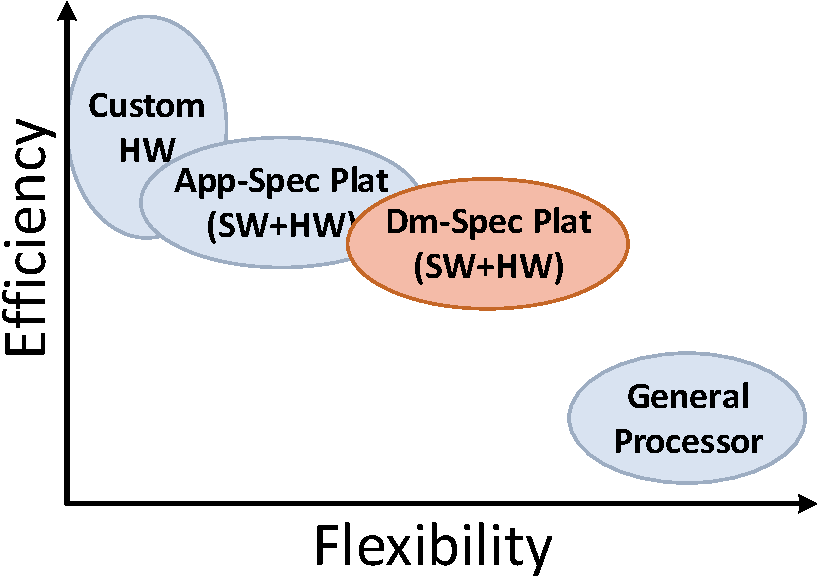
\includegraphics[width=.6\linewidth]{fig/pTradeOff.pdf}
	%\vspace{-6pt}
	\caption{Flexibility / Efficiency Trade-Off}
	\label{fig:tradeOffArch}
	%\vspace{-4pt}
\end{figure}


%\begin{wrapfigure}{l}{0.5\linewidth}
%	%\vspace{-6pt}
%	\begin{center}
%		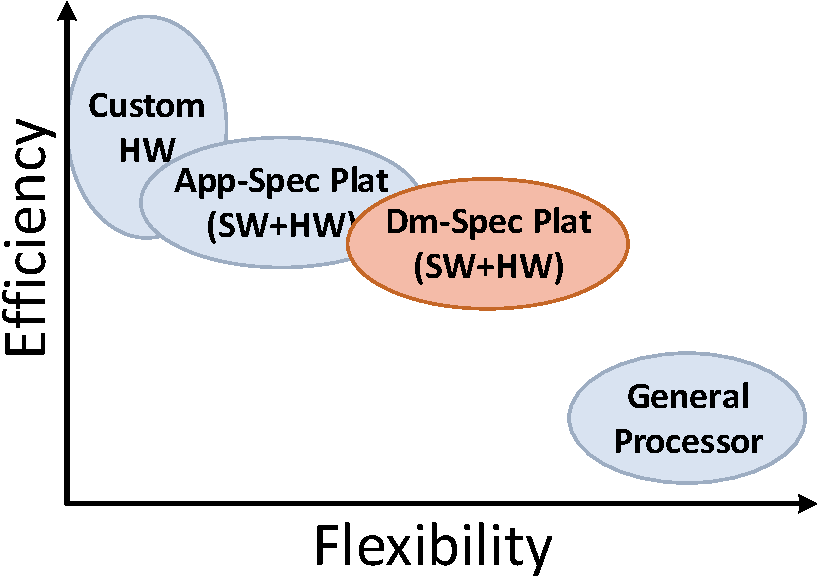
\includegraphics[width=\linewidth]{fig/pTradeOff.pdf}
%	\end{center}
%	%\vspace{-10pt}
%	\caption{Flexibility / Efficiency Trade-Off}
%	\label{fig:tradeOffArch}
%	\vspace{-4pt}
%\end{wrapfigure}

%\begin{figure}[t]
%    \centering
%    \subfloat[Flexibility / Efficiency]{
%       	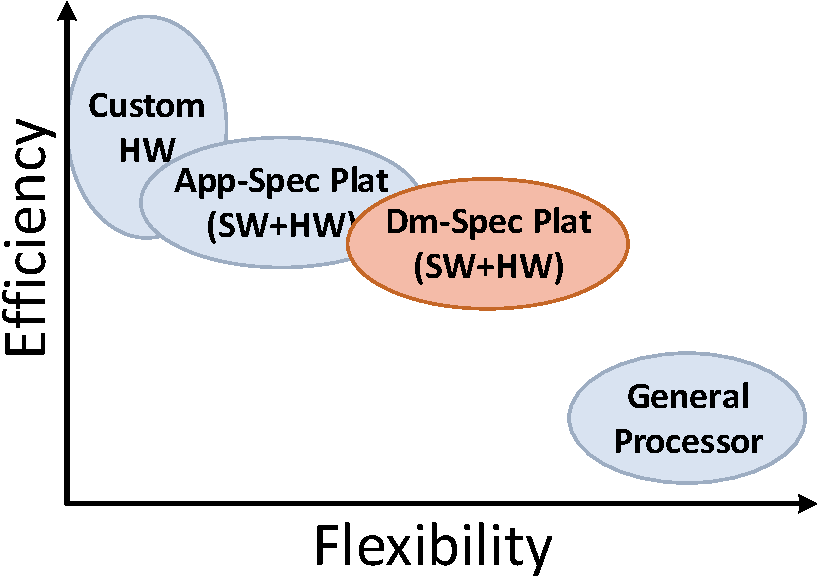
\includegraphics[width=.48\linewidth]{fig/pTradeOff.pdf}
%       	\label{fig:tradeOffArch}}
%    \hfill
%    \subfloat[Exploration / performance]{
%       	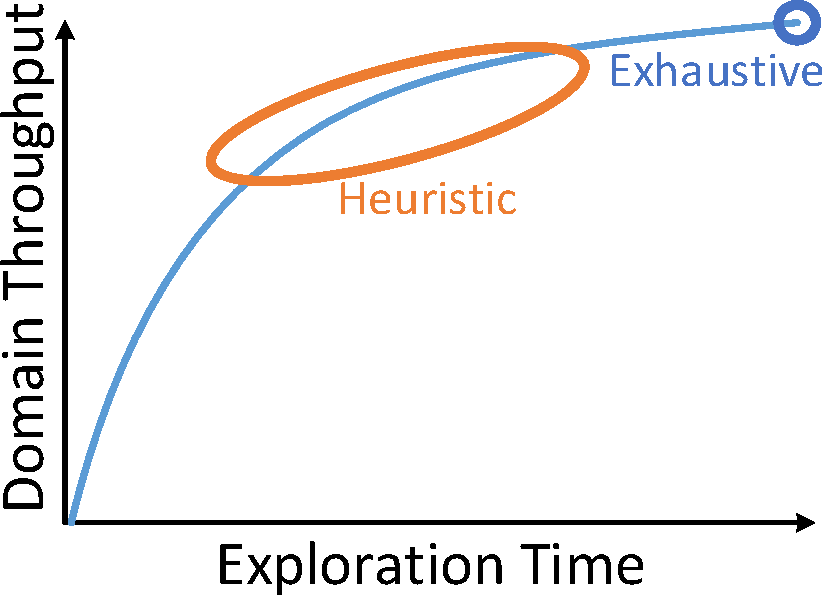
\includegraphics[width=.48\linewidth]{fig/pTradeOffAlg.pdf}
%       	\label{fig:tradeOffAlg}}
%		\vspace{-10pt}
%	\caption{Trade-Off for Platform and DSE}
%    \label{fig:trade-off}
%	\vspace{-10pt}
%\end{figure}

\begin{figure}[b]
		%\vspace{-20pt}
    \centering
        \subfloat[App-Specific Platform]{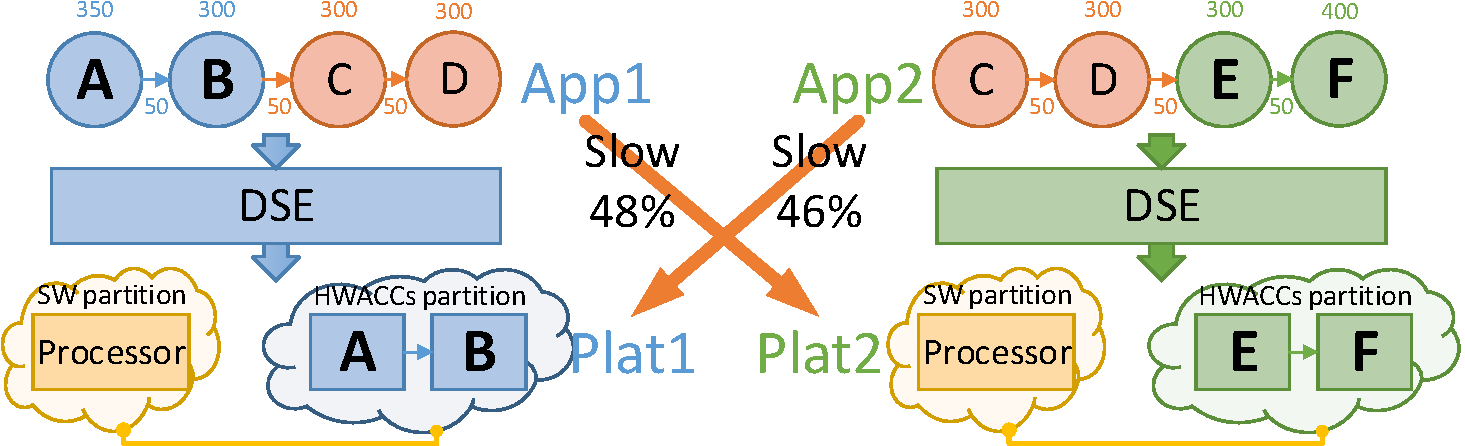
\includegraphics[width=.80\linewidth]{fig/pPlatApp.pdf}\label{fig:platApp}}
        \\ \vspace{-6pt}
        \subfloat[Domain-Specific Platform]{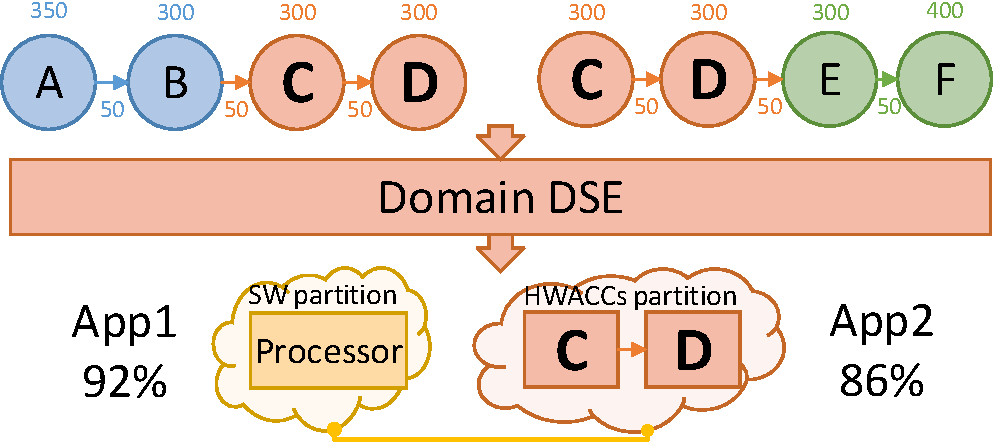
\includegraphics[width=.5\linewidth]{fig/pPlatDS.pdf}\label{fig:platDS}}
		%\vspace{-10pt}
    \caption{Domain Platform: Penalty of Application Scope}
    \label{fig:example}
\end{figure}


When moving to domain-platforms, few large monolithic accelerators make way for many smaller, composable accelerators. They offer configurable acceleration for selected compute-intensive kernels while running the remaining application in SW. Early domain-specific platforms include ACC-rich MPSoC~\cite{cong2014accelerator} or the Function-Level Processor~\cite{tabkhi2016function}. Domain-specific platforms aim at more specialization than typically considered in the platform-based design process, and target hardened implementations as opposed to reconfigurable computing  \cite{wildermann2011operational} paradigms.

%\figref{fig:tradeOffAlg} plots a domain DSE trade-off between exploration time and achievable domain throughput which is the result of identified domain function kernels for hardware acceleration. An exhaustive DSE throughout all possible design options (HW/SW choices over entire domain) can achieve the optimal domain throughput in the cost of excessive exploration time. Heuristic domain DSE algorithms are required that can offer near optimal accuracy with much shorter exploration time (traversing heuristic curve) to guide platform architects for finding the right balance and  HW/SW combinations for a domain.

Designing domain-specific platforms poses new challenges. 
While mapping multiple applications on an existing platform already received significant attention   \cite{kuang2005partitioning,wu2006low,abdeen2014multi,tang2015hardware}, 
designing domain platforms is less studied. 
Current DSE approaches primarily focus on a single application (one task graph) in isolation and do not address the domain optimization opportunities. 
The penalty of the narrow application focus is illustrated in \figref{fig:platApp}. Two platforms are each customized for an individual application, one accelerating $A$, $B$ and the other $E$, $F$. Executing each app on the other's platform results in low performance (48\%, 46\%).  Broadening the scope and considering both applications has tremendous benefits. The domain platform in \figref{fig:platDS} accelerates $C$, $D$ common to both applications. Now, both applications benefit from customization and execute at performance close to the own dedicated platform (92\%, 86\%). In order to explore the benefits of domain-specific platforms,  novel domain DSE tools and methodologies are needed that can identify functional and structural similarities across domain applications, utilize them for domain specialization, and rapidly evaluate the potential benefits for applications within a domain.

\newtext{This paper introduces a domain-specific design flow to aid HW/SW partitioning when designing a platform for a set of applications. The key insight is to identify both behavioral (functional) and structural similarities across applications in a domain, and then evaluate benefits of the similarities in Domain DSE for HW/SW partitioning to optimize performance across all domain applications.}

\newtext{This paper introduces two novel Domain-Specific DSE approaches, Dynamic Score Selection (DSS) and GenetIc Domain Exploration (GIDE), to enable the domain-specific platform design. They focus on streaming applications (e.g. video analytics, software defined radio) targeting platforms with many accelerators for high performance and power-efficient computing. Both, DSS and GIDE, broaden the scope of DSE from an individual application to a domain of applications. Instead of rigidly optimizing for a single application, the aim is to find a common platform that balances acceleration for a set of applications.}

\newtext{DSS is a very high-level, greedy approach. It introduces Domain Score (DS), a heuristic for estimating the variation in benefits for the whole domain at once when changing HW/SW allocation.} \ga \newtext{ improves domain evaluation accuracy over DS using high-level analytic models estimating each application individually.    
In addition,} \ga speeds up traversing the enormous design space using guided local search with a hybrid evaluation combining DS and Analytic Evaluation (AE). \newtext{Both approaches are evaluated in detail to highlight their characteristics and benefits. Their trade-off in exploration speed and accuracy is quantified. To the best of our knowledge, DSS and GIDE are the first greedy and genetic algorithms for domain design space exploration. 

In a nutshell, the contributions of this paper are:}

%This paper introduces GenetIc Domain Exploration (\ga), a novel Domain-Specific DSE enabling the domain-specific platform design process.
%\ga focuses on streaming applications (e.g. video analytics and software define radio) targeting platforms with many accelerators. \ga broadens the scope of Genetic Algorithms (GA) from an individual to a domain of applications. It defines assessing the benefit of a domain platform for its applications as the average throughput improvement over all applications. To speed up performance analysis in the evaluation, \ga utilizes high level analytical models. \ga speeds up traversing the enormous design space using guided local search with a hybrid evaluation combining Domain Score (DS) and  Analytic evaluation. In addition, its individual evaluation approaches are evaluated in detail to quantify their benefits in speed and accuracy. To the best of our knowledge, \ga is the first genetic algorithm for domain design space exploration. In a nutshell, the contributions of this paper are:

\begin{enumerate}
    \item Defining quantifiable domain features to express the similarities among applications.
    \item Providing a domain analyzer to extract domain features from applications.
    \item Introducing Domain Score (DS) to compare relative benefit of a platform in domain level.
    \item Accelerating the evaluation of domain-platforms fitness for a group of applications through Analytic Evaluation (AE).
    \item Introducing the first greedy algorithm Dynamic Score Selection (DSS) using DS for rapid Domain-Specific Design Space Exploration (DS-DSE).
    \item Introducing the first genetic algorithm GenetIc Domain Exploration (GIDE) for DS-DSE. In \ga, accelerating the design space traversal through guided local search using a hybrid of DS and AE.
    \item Providing a methodology to evaluate platforms in context of domains.
    \item Exploring the speed versus accuracy trade-off for domain exploration.
\end{enumerate}

%One major contribution of this paper encoding domain platform options to GA chromosomes coupled with the guided local search to narrow down the domain design space. For the GA guided local search, this paper proposes two domain evaluation options: (1)  which offers faster evaluation, but lower accuracy. (2) Analytical which offers higher accuracy but slower evaluation. The GA algorithm is coupled with multiple variations of guided local search (DSS, analytical, or hybrid) to create a balance between domain exploration time and evaluation accuracy (which can lead to higher domain throughput). 
%JH comment: There is no clear contribution summary in Introduction.

The benefits of DSS and \ga are demonstrated using 40 applications from the video analytics domain based on OpenVX \cite{Intel, AMD}, as well as varying synthetic domains. \newtext{Results are compared against application-specific designs and domain optimal results (obtained through exhaustive search) wherever possible.}
\newtext{The DSS} and \ga generated platforms significantly improve performance: 23.60\%-58.02\% and 48.09\%-74.85\% on average compared to application-specific platform designs.
\newtext{DSS achieves 93.65\% and 83.45\% of domain optimal throughput for OpenVX and synthetic domain}. \newtext{GIDE further improves performance, reaching 99.87\% and 98.84\% of domain optimal throughput. The higher performance of} \ga \newtext{comes at the cost of longer design space exploration time ($10^{13}$ instead of $10^{17}$ times faster than exhaustive search).}
With this, \ga enables rapid domain design space exploration producing high quality results.

%The benefits of \ga are demonstrated using 40 applications from the video analytics domain based on OpenVX \cite{Intel, AMD}, as well as varying synthetic domains. Results are compared against optimal results (obtained through exhaustive search) wherever possible, and an existing heuristic approach - Domain Score Selection (DSS)~\cite{zhang100ds}. \ga reaches 99.8\% and 97.6\% of domain optimal throughput for OpenVX and synthetic domains, with $10^{13}$ times faster exploration than exhaustive search. 
%Compared to the greedy DSS, \ga achieves 10.65\%  and 19.81\% higher domain throughput improvement for OpenVX and synthetic domains. With this, \ga enables rapid domain design space exploration producing high quality results.

\begin{figure}[h]
	\centering
	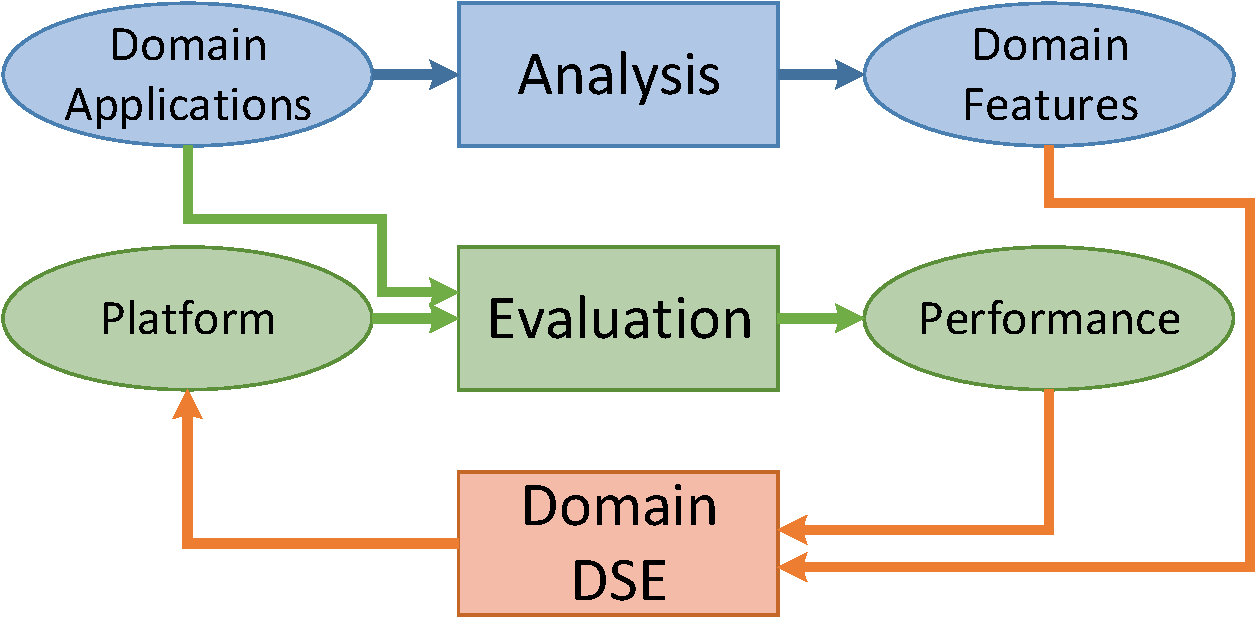
\includegraphics[width=.65\linewidth]{fig/Overview.pdf}
	\caption{Domain DSE Overview}
	\label{fig:overview}
\end{figure}

\newtext{
\figref{fig:overview} illustrates the flow and principle steps of Domain DSE. It also serves as a blueprint of this journal's structure. 
The basis of exploration is a set of domain features extracted from domain applications through analysis. For this,  \secref{sec:Domain}, highlighted in blue, identifies domain features, metrics and presents domain features analyzer. In order to quantify the benefits of a platform for a set of applications, \secref{sec:EvaOp} defines an evaluation methodology and appropriate metrics (highlighted in green). It introduces the target domain platform and the proposed platform evaluation models. The Domain DSE is tackled in \secref{sec:DSE}, which defines the exploration problem, and \secref{sec:Domain}, which introduces efficient domain-level DSE algorithms traverse and explore the large domain design space. For the later, \secref{sec:DSS} describes the high level DSS HW/SW partitioning, and \secref{sec:GA} introduces \ga with an iterative genetic-algorithm-based search assisted by a guided local search. \secref{sec:results}  evaluates and analyses both approaches with a detailed performance analysis and insights. 
%\secref{sec:generalization} summarizes all algorithms in DSE trade-off. 
Finally, \secref{sec:conclusion} concludes this paper. }
\section{Related Work}
\label{sec:related}
Optimizing HW/SW partitioning for individual applications has received much research attention. For a limited design space, exact algorithms, such as integer linear programming \cite{kuang2005partitioning}, branch-and-bound \cite{jigang2004branch}, and dynamic programming \cite{wu2006low}, guarantee to find the optimal solution. For complex design spaces, this is an NP-hard problem, heuristics are the only viable approach (however without guaranteeing to find the optimum). Examples are genetic algorithms (GA) \cite{quan2014towards, alexandrescu2011genetic, wen2011heuristic, page2010multi}, simulated annealing \cite{liang2013hardware}, tabu search \cite{wu2013efficient}, and greedy algorithms \cite{tang2015hardware}. 

GA-based heuristics for design space exploration is a rich research area. Some approaches, e.g. \cite{quan2014towards}, keep the best solutions in each generation to orient the inheritance of good genes. GA with smart mutation \cite{alexandrescu2011genetic} uses platform knowledge to guide the mutation to increases the solution's convergence rate. The local search algorithm is also combined with GA \cite{wen2011heuristic} to accelerate the exploration speed. \cite{page2010multi} uses different heuristics initialization for getting better solutions. 
 
To accelerate the heuristic, a fast evaluation mechanism is essential. Existing heuristics either leverages analytical estimation \cite{pinedo2016scheduling, omara2010genetic}), or use abstract simulation and TLMs \cite{pimentel2006systematic, ghenassia2005transaction}. Some heuristics combine the benefits of analytical and simulation \cite{zhang2014automatic, mariani2010correlation}. They prune design space using analytical assumptions and then perform the simulation-based evaluation for the few design candidates.

Overall, existing DSE for creating new platforms focuses on a single application in isolation. Some ideas toward a domain focus can be extracted from platform-based computing which uses statistical information for destining the platform and application-specific mapping \cite{graf2014multi, gladigau2010system}. However more specialization for a wider set of applications is needed. Reconfigurable computing, such as  \cite{wildermann2011operational}, aims to support multiple applications one at a time, however does need to rely of functional and structural similarities across reconfiguration cycles. 

An early example of domain exploration is Domain Score Selection (DSS) \cite{zhang100ds} which proposes a greedy approach for identifying domain function kernels for hardware acceleration. While \cite{zhang100ds} is very promising in terms of formalization and definitions, the achieved performance however is bounded by limitations of the greedy approach.

%There is no clear path to broaden their scope to domain DSE.  which is not really accuracy only using simple score calculation to guide the approach. The domain DSE needs an efficient algorithms to explore the large domain design space. Fast and accuracy evaluation method to evaluate the efficiency of domain platform for all applications


\section{Domain Formalization}
\label{sec:Domain}

The foundation of any systematic approach for domain-specific-DSE is the formalization of a domain and its features (metrics) to quantitatively reason about the domain. This section defines the domain scope and its features (metrics). They capture the behavioral and structural features of a domain showing what functions are commonly used and how they are composed. Defining these features and metrics lays the foundation for automatic domain analysis and exploration.

\subsection{Domain Definition}
\label{sub:dmDefine}
Domain is a set of applications, which share common functions and common patterns\cite{kang1990feature}. To allow reasoning about the domain\footnote{Defining the scope of a domain, i.e. assessing domain membership, is an additional research topic.}, we formally define it as a set of graphs.
%Current definitions of domain include a set of applications which share a set of common capabilities and data \cite{kang1990feature}, a class of applications, with a component library, which contains reusable chunks of domain expertise \cite{tracz1995dssa}. Following this definition, we define a domain as a set of applications, which share common functions and common patterns. To allow reasoning about the domain\footnote{Defining the scope of a domain, i.e. assessing domain membership, is an additional research topic.}, we formally define it as a set of graphs.
%\vspace{-5pt}
\begin{equation}
\begin{split}
\label{eq:domain}
	&G = \{g_{0}, g_{1}, ..., g_{N}\}, \quad g_{i} = (A, E)\\
	&A = \{a_{0}, a_{1}, ..., a_{n}\}, \quad E = \{e_{0}, e_{1}, ..., e_{m}\}\\
	&a_{i} (t, d_{P}), \quad e_{i} ((a_{src}, a_{dst}), d_{C})
\end{split}
\end{equation}
%\endgroup
%\vspace{-10pt}

In Eq.~\eqref{eq:domain}, domain $G$ is a set of streaming applications ($g_{0}$ .. $g_{N}$), each captured as a dataflow graph \cite{stuijk2006sdf}. Each application $g_i$ contains a set $A$ of processing actors ($a_0$ .. $a_n$) and a set of $E$ edges ($e_0$ .. $e_m$) representing the communication between actors. Each actor $a_i$ is an instance of a function type $t$ with an instance-specific processing demand $d_{P}$ (\# of operations). Multiple instances of the same function type $t$ may exist within and across applications within the domain. Each edge $e_i$ is the directed communication between its $a_{src}$ and $a_{dst}$ with a communication demand of $d_{C}$ as a measure of the transferred volume (bytes). E.g., in application $g0$ of Fig.~\ref{fig:Apps}, the first actor $A0$ is an instance of $t_{A}$ and its $d_{P} = 350$, and the edge between $A0$ and $B0$ contains $d_{C} = 50$. 

\begin{table}[h]
  \begin{minipage}[b]{0.35\linewidth}
    \centering
    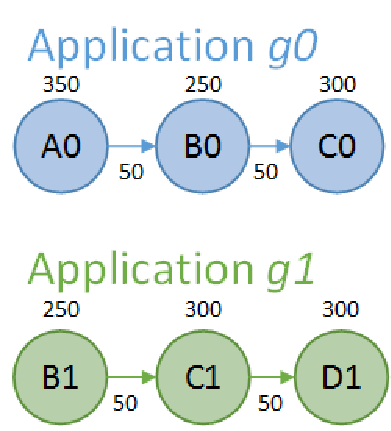
\includegraphics[width=0.9\linewidth]{fig/Apps.pdf}
    \captionof{figure}{Example: Domain Applications}
    \label{fig:Apps}
  \end{minipage}
	 \hfill
  \begin{varwidth}[b]{0.6\linewidth}
    \centering
    \begin{tabular}{l r r r}
      \toprule
      Composition & $P$ & $D_{P}$ & $D_{C}$ \\
      \midrule
      $\{t_A\}$ & 50\% & 350 & -- \\
      $\{t_B\}$ & 100\% & 500 & -- \\
      $\{t_C\}$ & 100\% & 600 & -- \\
      $\{t_D\}$ & 50\% & 300 & -- \\
			\hline
			$\{t_A,t_B\}$ & 50\% & -- & 50 \\
			$\{t_B,t_C\}$ & 100\% & -- & 100 \\
			$\{t_C,t_D\}$ & 50\% & -- & 50 \\
			\hline
			$\{t_A,t_B,t_C\}$ & 50\% & -- & -- \\
			$\{t_B,t_C,t_D\}$ & 50\% & -- & -- \\			
      \bottomrule
    \end{tabular}
    \caption{Example: Domain Features}
    \label{tab:egFeature}
  \end{varwidth}
\end{table}
\subsection{Domain Features}
\label{sec:features}
Domain features lay the foundation for automatic exploration. It is essential to capture behavioral similarity to assess processing needs, and structural similarities to assess communication / topology requirements. Aligned with the domain definition, we identify commonly used functions and function patterns. We express common functions as the function types of actors that repeat within and across applications. Function patterns are repeating compositions these function types (i.e. identical subgraphs). Different lengths of compositions are considered. For example, application $g0$ in Fig.~\ref{fig:Apps}, has three, two and one composition of a degree one, two and three, respectively. The function type composition $\{t_{B}, t_{C}\}$ (which is of degree 2) appears in application $g0$ (actors $B0$,$C0$) and $g1$ ($B1$,$C1$). \tabref{tab:egFeature} lists the compositions of the domain.

%removed the detour of instances. Directly explained it as types. no addl. formula neede
%The definitions of actor composition $c$ and function type composition $C$ are given in Eq.~\ref{eq:comps}.   
%
%\vspace{-10pt}
%%\begingroup\makeatletter\def\f@size{9}\check@mathfonts
%\begin{equation}
%\begin{split}
%\label{eq:comps}
	%c = \{a_j, a_k,...\}, \quad C = \{t_J, t_K,...\}\\
%\end{split}
%\end{equation}
%%\endgroup
%%\vspace{-10pt}

A composition of degree one ($\left\vert{C}\right\vert = 1$) contains a single function type. All compositions $\left\vert{C}\right\vert = 1$, represent the function types shared across the domain. Since compositions $C$ can capture both common functions (behavioral similarity) and function patterns (structural similarity), this paper chooses function type compositions $C$ to express domain features. In addition to the subgraph of function types, we focus on three aspects to characterize compositions: probability of appearance, processing demand and communication demand. 

Compositions that appear more often across applications are more important for the domain than infrequent compositions. To quantify the importance, we define appearance probability $P$ as per Eq.~\eqref{eq:p}. 

%\vspace{-10pt}
\begin{equation}
\begin{split}
\label{eq:p}
P(C_i) = (\sum_{g_j \in G} \left\vert \{ Instance(C_i) \in g_j \} \right\vert) / \left\vert{G}\right\vert \\
%	P(C) = \left\vert{ \{g \vert c \in g, c \in C \} }\right\vert / \left\vert{G}\right\vert \\
\end{split}
\end{equation}


$P$ is probability that an instance of composition $C_i$ appears in a domain application. The composition $\{t_{B}, t_{C}\}$ in Fig.~\ref{fig:Apps} and Table~\ref{tab:egFeature} appears in all applications ($P$ = 100\%). Whereas $\{t_A, t_B\}$ and $\{t_C, t_D\}$ each appear only in one ($P$ =50\%).  

A key challenge to enable domain DSE is how to identify processing and communication demands across applications which are necessary to guide resource allocation. However, considering each individual application is impractical. To obtain a domain-level view, we aggregate the demands for each composition as defined in Eq.~\eqref{eq:demand}.

%\vspace{-8pt}
\begin{equation}
\begin{split}
\label{eq:demand}
	&D_P(C_i=\{t_j\}) = \sum_{g_k \in G} \sum_{ a_l = Instance(t_j) \in g_k} a_l.d_P\\
	&D_C(C_i=\{t_i, t_j\}) = \sum_{g_k \in G} \sum_{e_l \in g_k, e_l=\{t_i,t_j\}} e_l.d_C
\end{split}
\end{equation}
%\vspace{-10pt}

%In general, DSE compares the processing workload $d_P$ among computing actors to decide which to accelerate and analyzes the communication $d_C$ between them to avoid data transfer. However, the individual $d_P$ and $d_C$ is a mess for DS-DSE. The DS-DSE needs the features in domain level to decide the partitioning of function types. 

The processing demand $D_P$ is calculated for each composition $C_i$ with a degree of one as the sum over all applications and all instances of the type $t_j$ (e.g. $D_P(t_B)$ = 500). Communication demand is computed for each pair of actor types (i.e. compositions of degree two). It is the sum of the communication demand for each edge of that type over all applications ($D_C(\{t_B, t_C\})$ = 100). 

%\vspace{-10pt}
\begin{equation}
\begin{split}
\label{eq:CS}
	&CS = \{C_{0}, C_{1}, ..., C_{z}\}\\
	&C_{i} (P, D_P, D_C)\\
\end{split}
\end{equation}
%\vspace{-10pt} 

In summary, the domin features are captured as a set of compositions, where each composition $C_i$ is defined by its appearance probability $P$, processing demand $D_{P}$ (for $\left\vert{C_i}\right\vert = 1$), and communication demand $D_{C}$ (for $\left\vert{C_i}\right\vert = 2$).
Table~\ref{tab:feature} shows the general view of the selected domain features. 

%GSTODO table is redundant in my view
\begin{table}[h]
	\caption{Domain Features}
	\label{tab:feature}
	\centering
	\begin{tabular}{p{0.06\linewidth}|p{0.22\linewidth}|p{0.15\linewidth}|p{0.15\linewidth}|p{0.18\linewidth}}
		\toprule
		\multicolumn{2}{c|}{Composition}& Appearance Probability& Processing Demand& Communication Demand\\
		\midrule
		\hline
		$C_{0}$&				$\{t_{A}\}$&								$P(C_{0})$&					$D_{P}(C_{0})$& --\\
		$C_{1}$& 				$\{t_{B}\}$&								$P(C_{1})$&					$D_{P}(C_{1})$& --\\
		$...$& 					$...$&									$...$&							$...$&	--\\
		$C_{x}$& 				$\{t_{N}\}$&								$P(C_{x})$&					$D_{P}(C_{x})$& --\\
		\hline
		$C_{x+1}$& 			$\{t_{A}, t_{B}\}$&					$P(C_{x+1})$&				--& $D_{C}(C_{x+1})$\\
		$C_{x+2}$& 			$\{t_{A}, t_{C}\}$&					$P(C_{x+2})$&				--& $D_{C}(C_{x+2})$\\
		$...$& 					$...$&									$...$&							--&			$...$\\
		$C_{y}$& 				$\{t_{I}, t_{N}\}$&					$P(C_{y})$&					--& $D_{C}(C_{y})$\\
		\hline
		$C_{y+1}$& 			$\{t_{A}, t_{B}, t_{C}\}$&		$P(C_{y+1})$&				--&	--\\
		$...$& 					$...$&									$...$&							--&	--\\
		$C_{z}$& 				$\{t_{I}, t_{J}, ...,t_{N}\}$&		$P(C_{z})$&					--&	--\\
		\bottomrule
	\end{tabular}
\end{table}
\subsection{Domain Analyzer}
\label{sec:analyzer} 

\newtext{To obtain domain features, domain analyzer extracts the behavioral and structural similarities from the applications within a domain. It expresses these similarities using the domain features defined in} \secref{sec:features}. The computed domain features then feed into our domain-specific DSE described in \secref{sec:DSE}.
%This paper primarily focuses on streaming applications, which have significant functional and structural similarities within a domain. The extracted similarities 

Algorithm~\ref{alg:analysis} overviews the domain analyzer. The analyzer is comprised of domain analysis and application analysis. The domain analysis (lines 1-11) first calls application analysis for each application to obtain the list of function type compositions ($CList$ in line3). Then the domain analysis merges compositions from all applications, counts their appearance frequency (lines 4-8), and aggregates their processing and communication demand ($D_P, D_C$ in line 9). Finally, the domain analysis calculates each composition appearance probability ($P$ in line 11) and returns the the domain features as a set of function type compositions.

\begin{algorithm}
\caption{Domain Analyzer}
\label{alg:analysis}
\begin{algorithmic}[1]
{\footnotesize
\Function{dmAnalysis}{$G$}
	\For{\textbf{each} $g \in G$}
		\State $CList = \Call{appAnalysis}{g}$
		\For{\textbf{each} $C \in CList$}
				\If {$C \in CS$}
					\State $Freq(C)$++
				\Else
					\State $CS = CS \cup \{C\}; Freq(C) = 1$
				\EndIf
				\State $D_{P}(C)$ += $C.D_{P}; D_{C}(C)$ += $C.D_{C}$
		\EndFor
	\EndFor
	\For{\textbf{each} $C \in CS$}
		\State $P(C) = Freq(C) / \left\vert{G}\right\vert$
	\EndFor
	\Return $CS$
\EndFunction
\item[]
\Function{appAnalysis}{$g$}
	\For{\textbf{each} $a \in g.A$}
		\State $cList.add( \{a\} )$
	\EndFor
	\For{$k \in \{1,2,\dots\}$}
	\Comment $k$ is composition degree
		\For{\textbf{each} $c \in\{cList \cap \left\vert{c}\right\vert = k\}$ }
			\For{\textbf{each} $a_{next} \gets c.a_{tail}().a_{outNeighbor}()$}
				\If{$a_{next} \notin c$}
					\State $cList.add( c \cup \{a_{next}\} )$
				\EndIf
			\EndFor
		\EndFor
		\IIf {$\{c \vert c \in cList \cap \left\vert{c}\right\vert = k$+$1\} = \emptyset$} Break
	\EndFor

	\For{\textbf{each} $c \in cList$}
			\State $C$ = \{$a.t \vert a \in c$\}
			\IIf {$\left\vert{c}\right\vert = 1$} $C.D_{P} = a.d_{P},$ which $a \in c$
			\IIf {$\left\vert{c}\right\vert = 2$} $C.D_{C} = e.d_{C},$ which $ e.a_{src,dst} \in c$
			\If {$C \in CList$}
				\State $CList[C].updateD(C.D_{P},C.D_{C})$
			\Else
				\State $CList.add(C)$
			\EndIf
	\EndFor
	\Return $CList$
\EndFunction
}
\end{algorithmic}
\end{algorithm}

The application analysis (lines 12-28) creates a list of actor compositions (lines 12-20) and then abstracts from actor instances into function type compositions (lines 21-28). The analysis starts with each actor from the application as 1-degree composition (lines 13-14). Then for each $k$-degree composition, it adds one more actor to it to build a $k+1$ degree composition (lines 15-19). When no actor can be added anymore, actor compositions detection stops (line 20). After that, the analysis obtains a function type composition from each actor composition(lines 21-22). It merges duplicated function type compositions and aggregates their processing/communication demand (lines 23-28). It returns the list of compositions of this application, with their aggregated processing and communication demands. 
%The extracted similarities will be used as the input model for our proposed domain-specific DSE.






% GA domain formalization

%A domain is a set of applications, which share common functions and common patterns as introduced in \cite{zhang100ds}. Eq.~\ref{eq:domain} presents domain concept symbolically. A domain $G$ is a set of streaming applications ($g_{0}$ .. $g_{N}$), each captured as a dataflow graph \cite{stuijk2006sdf}. Each application $g_i$ contains a set $A$ of processing actors ($a_0$ .. $a_n$) and a set of $E$ edges ($e_0$ .. $e_m$) representing the communication between actors. Each actor $a_i$ is an instance of a function type $t$ with an instance-specific processing demand $d_{P}$ (\# of operations\footnote{To simplify explanation and clarity in result discussion, we abstract processing to a single dimension. More dimensions are possible and only affect the evaluation.}). Multiple instances of the same function type $t$ may exist within and across applications within the domain. A domain contains a set $T$ of function types. Each edge $e_i$ is the directed communication $a_{src}$ to $a_{dst}$ with a communication demand of $d_{C}$ (\# of transferred bytes). 

%\begin{equation}
%\begin{split}
%\label{eq:domain}
%	&G = \{g_{0}, g_{1}, ..., g_{N}\}, \quad g_{i} = (A, E)\\
%	&A = \{a_{0}, a_{1}, ..., a_{n}\}, \quad E = \{e_{0}, e_{1}, ..., e_{m}\}\\
%	&a_{i} (t, d_{P}), \quad e_{i} ((a_{src}, a_{dst}), d_{C})\\
%		&T = \{t_{A}, t_{B}, ..., t_{X}\}
%\end{split}
%\end{equation}

% potentially move this defintion to GALS approach.
%Given the formalization, the problem can be defined as follows:
%\begin{problem}[DS-DSE]
%\label{p:dse}
%	\normalfont{Given a domain \textit{G} and a HW budget $N$ (area), find a HW/SW partition of \textit{T} (the set of domain function types) that maximizes average throughput improvement over pure SW execution for all $\textit{g} \in \textit{G}$.}
%\end{problem}
\section{Domain Platforms Evaluation}
\label{sec:EvaOp}

To set the stage for our proposed domain DSE approach \newtext{(DSS and \ga)},
this sections introduces our assumptions / formalization about the
target platform in~\secref{sec:Platform}, \newtext{and different evaluation options of domain platform, Analytic Evaluation (AE)} in~\secref{sec:Ana} and Domain Score (DS) in~\secref{sec:ds}. ~\secref{sec:eva:sum} \newtext{discusses the accuracy and speed trade-off of these evaluation options.}

%\vspace{-4pt}
\subsection{Target Platform}
\label{sec:Platform}

To balance flexibility and efficiency, domain platform includes hardware accelerators (HWACC) and programmable processors (CPU, GPU, DSP), similar to current platforms. However, the number of HWACCs will increase dramatically, where individual HWACCs are less monolithic but smaller and configurable. HWACCs can be composed to accelerate larger kernels (or even applications), e.g. ACC-Rich MPSoCs \cite{cong2014accelerator} and FLP \cite{tabkhi2014function}. 

\begin{figure}[h]
	%\vspace{-4pt}
	\centering
	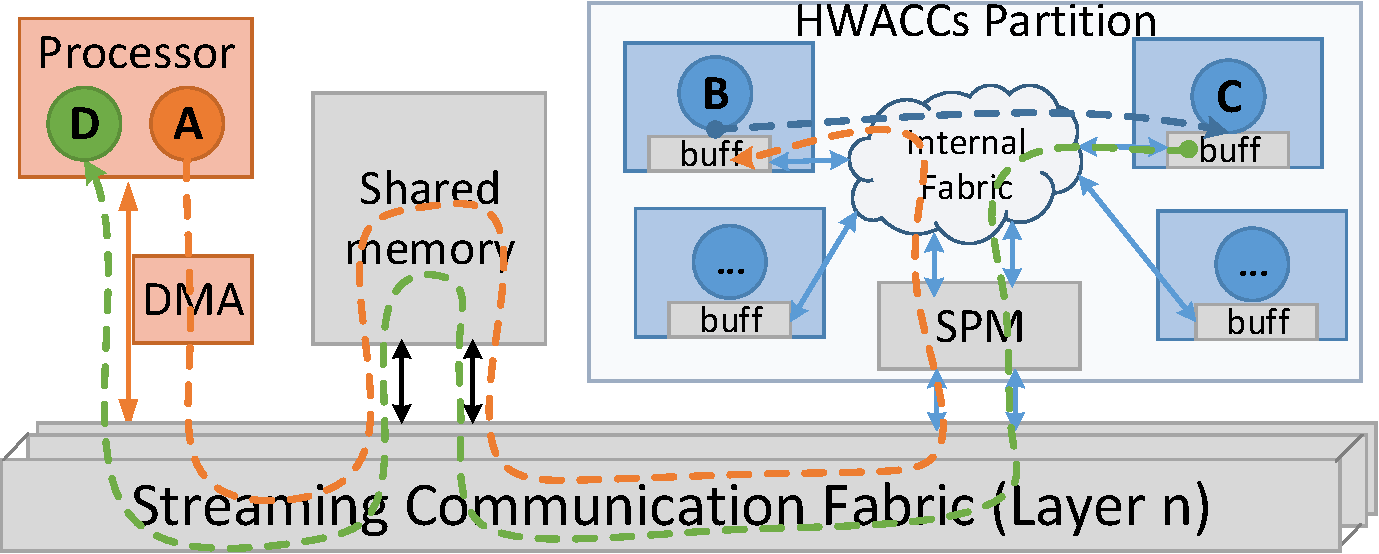
\includegraphics[width=.65\linewidth]{fig/pPlat.pdf}
	%\vspace{-6pt}
	\caption{Target Platform}
	\label{fig:plat}
	\vspace{-4pt}
\end{figure}

\figref{fig:plat} illustrates the target platform for the context of this work. A streaming application $A$,$B$,$C$,$D$ is mapped across SW and HW. Each HWACC has a dedicated SPM. All HWACCs are aggregated to a HW partition which a shared SPM across all HWACCs. HWACCs can communicate with each other; their communication traffic is hidden from system communication fabric (e.g. $B$, $C$). For simplicity, we assume direct n:n communication within the HW partition. Conversely, HWACCs and SW kernels communicate through the system streaming fabric (e.g. $A$ to $B$, and $C$ to $D$) which results in throughput penalties.


\newtext{Evaluating domain platforms is challenging due to the enormous design space needing to evaluate (a) the performance of each application given allocation and mapping, and (b) systematic aggregation across all applications to determine the platform benefit. For the purpose of this publication, we primarily focus on domain throughput improvement to assess the domain platform benefit. Domain throughput improvement is the average of all applications' throughput improvement each over their own pure SW implementation.} 

\newtext{Evaluating an individual application / platform follows a speed / accuracy trade-off. Transaction Level Models (TLM) can provide a reasonably high accuracy at cost of long simulation times limiting the number of evaluable design points in a given duration. More abstract and dramatically faster evaluation is desired to evaluate many more points at cost of accuracy.} 
~\secref{sec:Ana} and ~\secref{sec:ds} \newtext{propose two approaches and compares them against TLM simulation.}
\subsection{Analytic Evaluation}
\label{sec:Ana}

Performance analysis in context of DS-DSE is concerned about overall trends. Hence, the finer grained scheduling details of a TLM simulation are less important. As \ga targets streaming applications, the steady state performance is most important. 

The kernels in a streaming application operate as producers / consumers over the streaming data creating a pipeline. \figref{fig:Pipe} visualizes the pipeline execution for two HWACCs and one SW core. Each stage overlaps communication (in/out) with processing due to double buffering. Actors execute concurrently given their dependencies across different components. Actors mapped to the same component execute sequentially (e.g. in \emph{S8}).

Our analytical model computes the throughput of an application based on the inter-kernel pipelined execution~\cite{Teimouri_DAC_2015}.
At this abstraction, the throughput only depends on the pipe latency which is determined by the slowest processing component (or communication).

\begin{figure}[h]
	%\vspace{-10pt}
	\centering
	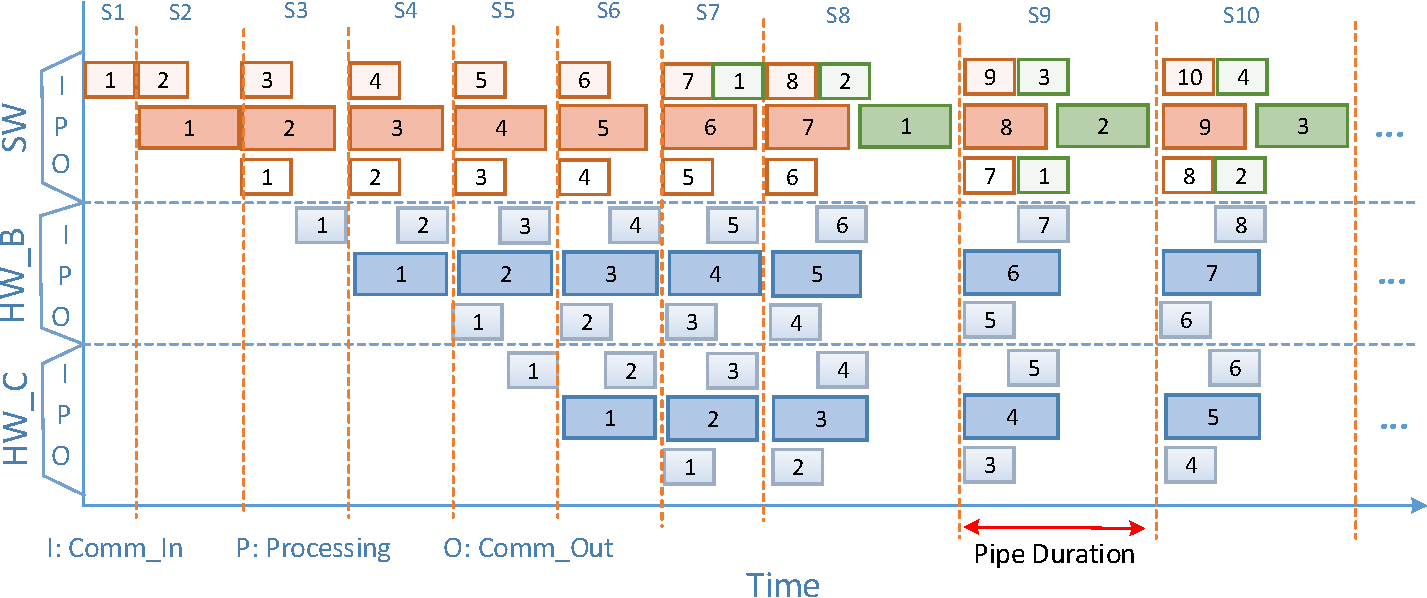
\includegraphics[width=\linewidth]{fig/pPipe.pdf}
	%\vspace{-10pt}
	\caption{Timing diagram of Architecture}
	\label{fig:Pipe}
	%\vspace{-6pt}
	
\end{figure}


Eq.~\eqref{eq:pipe} symbolically summarizes the analytical model. The estimated throughput is equal to output volume per iteration $D_{C}(out)$ over the pipe latency $L_{Pipe}$. \newtext{$L_{Pipe}$ is the maximum latency of SW ($L_{SW_i}$), HW ($L_{HW_j}$), and each layer of communication fabric ($L_{CE_k}$). }

\begin{equation}
\begin{split}
	&Throughput = D_{C}(out) / L_{Pipe} \\
	&L_{Pipe} = Max (\forall L_{SW}, \forall L_{HW}, \forall L_{CE}) \\
	&L_{SW_i} = \frac{\sum_{T \in SW_i} D_{P}(T)} {Freq_{SW}} + L_{sync} \\
	&L_{HW_j} = \frac{\sum_{T \in HW_j} D_{P}(T)} {Freq_{SW}*20} \\
	&L_{CE_k} = \frac{\sum_{C \in CE_k} D_{C}} {BW_{CE} * Freq_{CE}}
\label{eq:pipe}
\end{split}
\end{equation}

 \newtext{SW latency $L_{SW_i}$} is the accumulation of processing (i.e. total SW processing demand) and synchronization $L_{sync}$. Synchronization $L_{sync}$ is due to coordinating HW/SW communication including interrupt requests (from DMA, HW).
\newtext{HW latency $L_{HW_j}$} is due to processing an actor in HW. Each HWACC only executes one function type. 
The processing acceleration of an ACC depends on its frequency and the parallelism of the FT implemented on the ACC. For simplicity and clarity of explanation, this paper assumes a uniform HW acceleration of 20x. Non-uniform acceleration can be considered by defining an acceleration per function type.
\newtext{Communication latency $L_{CE_k}$} depends on the communication volume (between SW and HW) over bandwidth. Hence contention is only considered as an average. A multi-layer communication fabric is assumed. 
\subsection{Domain Score (DS)}
\label{sec:ds}

\newtext{For a rapid evaluation, an even higher abstraction level might be needed to gauge allocation / mapping benefits. For this, we develop the Domain Score (DS). Rather than estimating performance of an individual application on a platform, DS directly assesses costs and benefits of the platform to all applications in a domain.}
\newtext{DS relies on profiling all applications (only required once) to determine the total processing demand for each function type $D_P(t)$ and the communication demand between each function type pair $D_C(t_o,t_i)$. DS enables a relative comparison for incremental changes.} 
\newtext{DS quantifies the benefits of moving function types $t_{+}$ from SW to HW, and the penalties of moving $t_{-}$ from HW to SW with respect to processing and communication. In contrast to the analytic model, DS computes the score at once for the whole domain (i.e. incorporating all applications). No further aggregation and averaging are required.} 

%Given the amount of applications a domain and the myriad domain platform design options, a detailed simulations or detailed analytical approaches that include scheduling effects are prohibitively expensive to execute. Instead, our approach focuses on overall processing demand (i.e. how many operations) of the domain and processing supply by the architecture (symmetric for communication). The dynamic composition score quantifies the benefits moving a composition $C$ from processor to hardware mapping. DS estimates the benefits stemming from processing and communication mapping, scales them using dynamic weights (tuned to domain properties) and includes the additional cost of hardware implementation. 

%\vspace{-10pt}
\begingroup\makeatletter\def\f@size{9}\check@mathfonts
\begin{equation}
\begin{split}
\label{eq:scoreDS}
	Score &= B_{P} * w_{P} + B_{C} * w_{C}
	%cost &= \left\vert{C \cap SW}\right\vert
\end{split}
\end{equation}
\endgroup

In Eq.~\eqref{eq:scoreDS}, \newtext{$B_P$ and $B_C$ are the benefits of processing} and communication \newtext{when functions are changed in SW/HW mapping, respectively}. They are calculated considering aggregated benefits and appearances. $w_P$ and $w_C$ are the weights to scale both benefits. The weights are dynamically adjusted tracking performance bottlenecks, where processing or communication might be more important. Obtaining these weights will be discussed in Sec.~\ref{sub:weight}. %The $cost$ is defined the number of additional function types (i.e. HWACCs) to realize the composition in HW.


\subsubsection{Processing Benefit}
\label{sub:ben_proc}
Eq.~\ref{eq:comp} \newtext{estimates the processing benefit $B_P$ as execution time reduction / increase of the domain when mapping function types $t_{+}$ from SW to HW and $t_{-}$ from HW to SW, based on computation demand and supply.}

%\vspace{-10pt}
\begingroup\makeatletter\def\f@size{8.5}\check@mathfonts
\begin{equation}
\begin{split}
\label{eq:comp}
    B_{P} &= b_{P}(\{t_{+}\}) - b_{P}(\{t_{-}\}) \\
	b_{P}(X) &= \sum_{ t_{i} \in X } (\frac{D_{P}(t_{i})}{S_{SW}} - \frac{D_{P}(t_{i})}{S_{HW}}) * P(t_{i})
\end{split}
\end{equation}
\endgroup

In Eq.~\ref{eq:comp}, $S_{SW}$ and $S_{HW}$ are the estimated execution speed of SW and HW, respectively. \newtext{For each function type $t_{i}$ mapped from SW to HW, the overall difference of execution time between SW and and HW processing is calculated. This difference is then multiplied by the appearance probability $P$ of $t_{i}$ to prioritize frequently appearing compositions. The sum of the scaled processing benefits/disadvantage of these function types yields the processing benefit $B_P$ considering $t_{+}$ and $t_{-}$ switch.}
 
\subsubsection{Communication Benefit}
\label{sub:ben_comm}
The communication benefit is defined as the change in bus usage (transfer delay) due to switch mapping between sW and HW. It considers four aspects: \newtext{(1) $t_{+}$ saved communication with other HW-mapped functions, (2) $t_{+}$ additionally exposed HW/SW communication with other SW-mapped functions, (3) $t_{-}$ exposed SW/HW communication with other HW-mapped functions, and (4) $t_{-}$ saved communication with other SW-mapped functions. Communication between SW-mapped functions is assumed to be hidden in the memory hierarchy.} 

%\vspace{-10pt}
\begingroup\makeatletter\def\f@size{8.5}\check@mathfonts
\begin{equation}
\begin{split}
\label{eq:comm}
    B_{C} &=  b_{C}(\{t_{+}\}, HW \setminus \{t_{-}\}) - b_{C}(\{t_{+}\}, SW \setminus \{t_{+}\}) \\
        &- b_{C}(\{t_{-}\}, HW \setminus \{t_{-}\}) + b_{C}(\{t_{-}\}, SW \setminus \{t_{+}\}) \\
    b_{C}(X, Y) &= \sum_{ t_{i} \in X, t_{j} \in Y } D_{C}(t_{i},t_{j}) / S_{C} * P(t_{i},t_{j})
\end{split}
\end{equation}
\endgroup

Eq.~\eqref{eq:comm} captures the communication benefits, assuming $S_C$ is the communication speed of buses. It computes the saved versus exposed data transfer volume $D_C$ on bus divided by the communication speed $S_C$ to yield the change transfer delay. The change in delay scaling with appearance probability and its accumulation across all applications yields the communication benefit $B_C$, which is the change in transfer delay for the whole domain.


\subsubsection{Dynamic Weights}
\label{sub:weight}
Communication and processing demands vary by domains. In result, e.g. for a processing dominated domains (e.g. computer vision) targeting processing has priority resulting in the biggest improvements. While the benefits computed before already capture some of it, a global domain scope is needed to weigh the importance of communication versus processing of the whole domain. To capture this, we define the weights $w_C$ and $w_P$. 
However, each mapping to HW alters the effective communication vs. processing split and may change the properties and bottlenecks of the remaining compositions in a domain. For example, once processing intensive compositions are mapped to HW, the remaining compositions are communication-intensive. Therefore, the weights cannot be static but must be dynamically updated in each iteration to adjust for past mapping decisions.
%\vspace{-5pt}

\begingroup\makeatletter\def\f@size{8.5}\check@mathfonts
\begin{equation}
\begin{split}
\label{eq:weight}
	&w_{P} = \frac{\sum_{t_{i} \in SW} D_{P}(\{t_{i}\}) }{ \sum_{t_{i} \in SW} D_{P}(\{t_{i}\}) + \sum_{ \{t_{i}, t_{j}\} \nsubseteq HW} D_{C}(\{t_{i},t_{j}\}) }\\
	&w_{C} = 1 - w_P\\	
\end{split}
\end{equation}
\endgroup

Eq.~\eqref{eq:weight} illustrates the dynamic weight calculation. It uses the total remaining domain processing and communication demand (not mapped to HW) to determine the current performance bottleneck. A higher total demand of non-mapped (i.e. SW) processing raises the processing weight $w_P$. Conversely, if communication dominates the remaining domain, the communication demand $w_C$ will increase. 

%\secref{sub:dcs} and \secref{sec:GALS-DSS} will use the DS in the context of the Dynamic Score Selection (DSS) and GenetIc Domain Exploration (GIDE) algorithms. Since DSS greedily choosing the most promising function types $t_{+}$ for HW implementation, the DS only calculates the benefit of $t_{+}$ and the cost of consumed HW budget. However \ga comparing the switch of function types ($t_{+}$, $t_{-}$) implementation between SW and HW within certain budget, then DS considers the effect of both $t_{+}$ and $t_{-}$, and ignores the cost of budget consuming.

%\begingroup\makeatletter\def\f@size{8.5}\check@mathfonts
%\begin{equation}
%\begin{split}
%\label{eq:score}
%Score &= ( B_{P} * w_{P} + B_{C} * w_{C} )\\
%B_{P} &= D_{P}(t_{+}) - D_{P}(t_{-}) \\
%B_{C} &= \sum_{t_{I} \in HW}^{} D_{C}(t_{I}, t_{+}) - D_{C}(t_{I}, t_{-}) \\
%&+ \sum_{t_{I} \in SW}^{} D_{C}(t_{I}, t_{-}) - D_{C}(t_{I}, t_{+}) \\
%%B_{C} &= \sum_{t_{I} \in HW}^{} ( D_{C}(t_{I}, t_{+}) - D_{C}(t_{I}, t_{-}) ) + \sum_{t_{I} \in SW}^{} ( D_{C}(t_{I}, t_{-}) - D_{C}(t_{I}, t_{+}) )\\
%w_{P} &= \frac{\sum_{t_{I} \in SW} D_{P}(\{t_{I}\}) }{ \sum_{t_{I} \in SW} D_{P}(\{t_{I}\}) + \sum_{ \{t_{I}, t_{J}\} \nsubseteq HW} D_{C}(\{t_{I},t_{J}\}) }\\
%w_{C} &= 1 - w_P
%\end{split}
%\end{equation}
%\endgroup


\subsection{Trade-off: Evaluation Speed / Accuracy }
\label{sec:eva:sum}

To compare the the evaluation approaches in terms of accuracy and speed, we analyze them for a set of 40 real vision applications on 100 different platforms (with the same HW budget=5) against execution on a cycle-approximate TLM. % please name the few
\tabref{tab:fidelity} illustrates the trade-off looking at fidelity instead of accuracy as the evaluation approaches are compare design alternatives. TLM is defined as 100\% fidelity for this comparison.

\begin{table}[h]
	\caption{Fidelity and Speed: DS, \newtext{AE}, TLM}
	\label{tab:fidelity}
	\centering
	%\vspace{-10pt}
	\begin{tabular}{r||c|c|c}
		\toprule
		  & \textbf{DS}& \textbf{AE}& \textbf{TLM}\\
		\hline
		\midrule
		\textbf{Fidelity} & 89.07\%& 95.68\%& 100\%\\
		\hline
		\textbf{Eval. App [s]} & $7.2*10^{-5}$ & $6.0*10^{-4}$ & $1.8*10^2$ \\
		\hline
		\textbf{Eval. Domain [s]} & $7.2*10^{-5}$ & $6.0*10^{-2}$ & $1.8*10^4$ \\
		\bottomrule
	\end{tabular}
\end{table} 

Fidelity drops with abstraction: AE with 95.68\% and DS with 89.07\%. At the same time, abstraction yields dramatic speedups of 6 orders of magnitude from TLM to AE and another order of magnitude to DS. When evaluating a whole domain, DS is even 3 orders of magnitude faster than AE (assuming 100 apps in the domain) due to inherently incorporating all applications. In result, DS is preferred for rapid analysis, whereas the AE if more accuracy is needed. TLM simulation is too slow for DS-DSE.
\section{Domain DSE}
\label{sec:DSE}

%This section proposes a novel domain-specific DSE for HW/SW partitioning for a domain of applications. The key insight is to broaden the scope of the exploration heuristic from a single app in isolation to a group of applications. In general, different optimization goals are possible, e.g. minimize power consumption or maximize throughput with various constraints (e.g. cost, area). In this work, we focus on throughput improvement for all applications within a certain HW budget.

In next \secref{sec:DSS} and \secref{sec:GA}, \newtext{this paper proposes two novel domain-specific DSE, DSS and GIDE,} for HW/SW partitioning for a domain of applications. The key insight is to broaden the scope of the exploration heuristic from a single app in isolation to a group of applications. In general, different optimization goals are possible, e.g. minimize power consumption or maximize throughput with various constraints (e.g. cost, area). In this work, we focus on throughput improvement for all applications within a certain HW budget.

Using the domain formalization in \secref{sec:Domain}, DSS and \ga address the problem as follows: 
\begin{problem}[DS-DSE]
	\label{p:dse}
	\normalfont{Given a domain \textit{G} and a HW budget $N$ (area), find a HW/SW partition of \textit{T} (the set of domain function types) that maximizes average throughput improvement \footnote{In DSE problem, there are multiple objectives, e.g. throughput, delay, power consumption, and area. To simplify problem and clarify result discussion, this paper only focuses on one objective throughput with the fixed area limitation (area). Multiple-objective DS-DSE problems will be in the future work.} over pure SW execution for all $\textit{g} \in \textit{G}$.}
\end{problem}


\section{Dynamic Score Selection (DSS)}
\label{sec:DSS}

This section introduces a new algorithm: dynamic score selection (DSS). It starts with a pure SW platform and then iterates through greedily selecting a composition candidate from domain features for HW realization. \newtext{Our greedy approach uses the Dynamic Composition Score (DCS: based on Domain Score) to estimate which composition is the most promising to improve domain performance considering cost.} This section, first introduces the dynamic composition score and then the DSS algorithm.


\subsection{Dynamic Composition Score (DCS)}
\label{sub:dcs}

Given the amount of applications a domain and the myriad domain platform design options, a detailed simulations or detailed analytical approaches that include scheduling effects are prohibitively expensive to execute. Instead, our approach focuses on overall processing demand (i.e. how many operations) of the domain and processing supply by the architecture (symmetric for communication). The dynamic composition score quantifies the benefits moving a composition $C$ from processor to hardware mapping. DCS estimates the benefits stemming from processing and communication mapping, scales them using dynamic weights (tuned to domain properties) and includes the additional cost of hardware implementation. 

%\vspace{-10pt}
\begingroup\makeatletter\def\f@size{9}\check@mathfonts
\begin{equation}
\begin{split}
\label{eq:scoreDSS}
	DCS &= ( B_{P} * w_{P} + B_{C} * w_{C} ) / cost\\
	cost &= \left\vert{C \cap SW}\right\vert
\end{split}
\end{equation}
\endgroup

In Eq.~\eqref{eq:scoreDSS}, $B_P$ and $B_C$ are the benefits of processing and communication if the composition is mapped on HW, respectively. \newtext{They are calculated considering both aggregated benefits and appearances, see}~\secref{sub:ben_proc} and ~\secref{sub:ben_comm}. \newtext{$w_P$ and $w_C$ are the weights to scale both benefits (}~\secref{sub:weight}). The weights are dynamically adjusted tracking performance bottlenecks, where processing or communication might be more important. Since the the DSS dynamic choosing the promising composition $C$ (multiple function types $t$) for HW implement, the consumed HW budget is need to be taken into account. The $cost$ is defined the number of additional function types (i.e. HWACCs) to realize the composition in HW. 



\subsection{DS-DSE with Dynamic Score Selection (DSS)}
\label{sub:dss}

Dynamic Score Selection (DSS) implements Domain DSE based on DCS (Sec.~\ref{sub:dcs}). Algorithm~\ref{alg:dss} illustrates the flow. DSS starts with a pure SW mapping (line 1-2) and then greedily select the best candidate for HW mapping. Candidates are all compositions (and their contained function types) of the domain (line 3). DSS evaluates their benefits using the DCS (line 5-8) given current mapping and selects highest scored candidate. With a positive score, ie. performance improvement (line9), it maps all its SW-mapped function types to HW (lines 10-12). Subsequently it updates candidates by removing HW-mapped compositions (line 13). The loop (starting at line 4) repeats until the HW budget is exhausted (line 4) or no further improvement is possible (all negative score) (line 15).

\begin{algorithm}
\caption{DSS: Dynamic Score Selection}
\label{alg:dss}
\begin{algorithmic}[1]
{\footnotesize
\State $SW \gets T$
\State $HW \gets \emptyset$
\State $Cand \gets \{C \vert C \in CS\}$
\Comment Candidates
\While{$\left\vert{HW}\right\vert < HWbudget$}
	\LineComment Processing/Communication weight calculation
	\State $(w_{P}$, $w_{C}) = weightCal(CS, SW, HW)$
	\LineComment Calculate each candidate $C$ score, return the highest
	\State $C = scoreHighest(Cand, CS, SW, HW, w_{P}, w_{C})$
	\If{$C.Score > 0$}
		\For{\textbf{each} $t \in C \cap SW$}
			\State $SW = SW \setminus \{t\}$
			\State $HW = HW \cup \{t\}$
		\EndFor
		\State $Cand = Cand \setminus \{C.t \vert C \subseteq HW \}$
	\Else
		\State Break \Comment No improvement
	\EndIf
\EndWhile
}
\end{algorithmic}
\end{algorithm}
\section{\ga}
\label{sec:GA}

Novel exploration approaches are needed that broaden the scope of DSE from single application to a domain of applications in order to design a domain-specific platforms. The enormous design space renders exhaustive search infeasible, requiring heuristics for sparse sampling. Genetic Algorithm is one of efficient heuristics algorithms with high flexibility. This section presents GenetIc Domain Exploration (\ga), a genetic algorithm with a guided local search.



%Using the domain formalization in \secref{sec:Domain}, \ga addresses the problem as follows: 
%\begin{problem}[DS-DSE]
%	\label{p:dse}
%	\normalfont{Given a domain \textit{G} and a HW budget $N$ (area), find a HW/SW partition of \textit{T} (the set of domain function types) that maximizes average throughput improvement \footnote{In DSE problem, there are multiple objectives, e.g. throughput, delay, power consumption, and area. To simplify problem and clarify result discussion, this paper only focuses on one objective throughput with the fixed area limitation (area). Multiple-objective DS-DSE problems will be in the future work.} over pure SW execution for all $\textit{g} \in \textit{G}$.}
%\end{problem}


This section introduces \ga stepwise with increasing complexity. It first introduces the baseline genetic algorithm \emph{\garand} which outlines general principles and configurations. It then extends the algorithm by \newtext{a guided local search (LS) with 3 versions} to enhance the exploration performance. 


%\vspace{4pt}
\subsection{\garand}
% overview the algorithm and introduce the main components. Each component is then described 
% in more detail in a separate paragraph. 


% reduce the white space between figure and text by 
% adjusting columnsep
% see: https://tex.stackexchange.com/questions/106144/adjusting-left-right-margins-of-a-wrapfig
	
%\begin{wrapfigure}{r}{0.5\linewidth}
%	\begin{center}
%		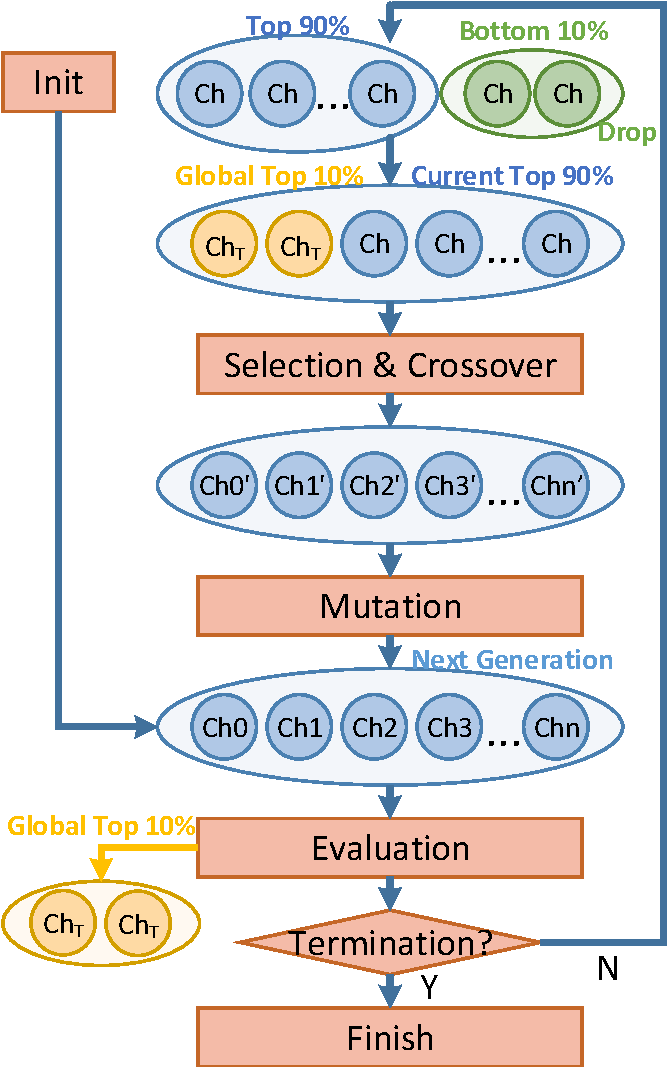
\includegraphics[width=\linewidth]{fig/pGA.pdf}
%	\end{center}
%	\vspace{-5pt}
%	\caption{Algorithm Overview}
%	\label{fig:GA}
%	%\vspace{-4pt}
%\end{wrapfigure}

\begin{figure}[h]
	\centering
	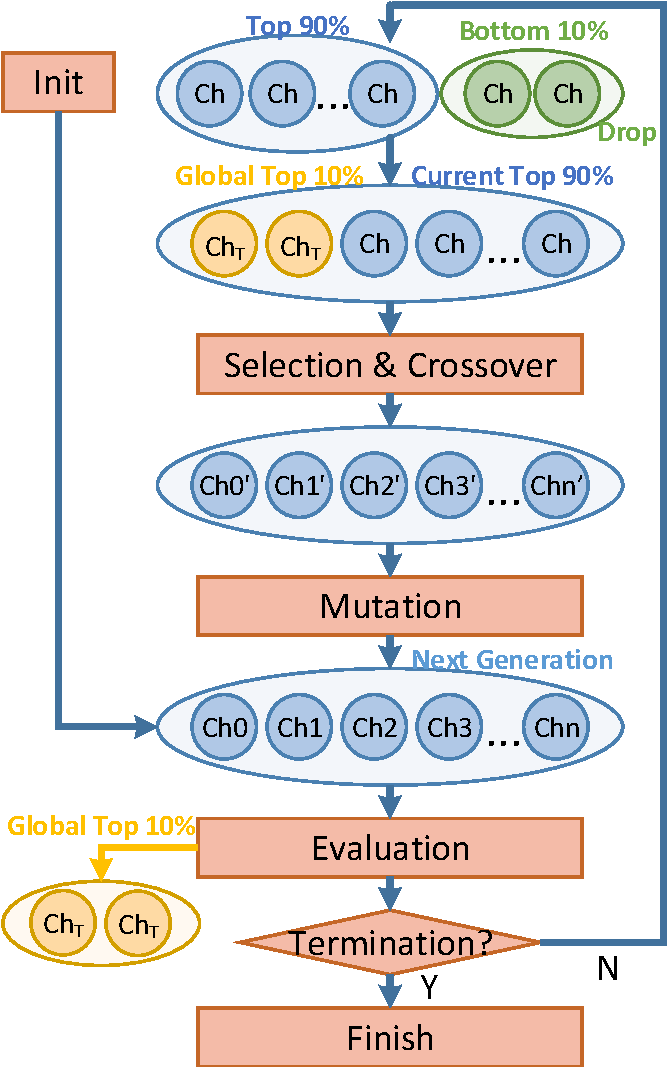
\includegraphics[width=0.5\linewidth]{fig/pGA.pdf}
	\caption{Genetic Algorithm Overview}
	\label{fig:GA}
\end{figure}

\figref{fig:GA} overviews our baseline genetic algorithm. The exploration configuration is captured in a set of \emph{chromosomes}. Each chromosome captures HW/SW mapping of each function type (FT) in the domain as a set of genes. After randomly generating an initial population, the \emph{evaluation} analyzes the fitness of each chromosome using the analytic model. The evaluation tracks global top 10\% chromosomes (across all generations). They replace the bottom 10\% in a generation to start a new population. From this, \emph{Selection \& Crossover} selects pairs of promising chromosomes swaps genes among them. To further increase variation, \emph{Mutation} randomly mutates individual genes. The resulting population is evaluated again and the process repeats until the \emph{Termination} condition is reached. The next paragraphs describe the process in detail. 



\textbf{Chromosome Definition.} An architecture is encoded as a chromosome as a string of integers, see Eq.~\eqref{eq:ch}, representing individual genes in a fixed order. Each gene ($g_A$, $g_B$ .. $g_X$) represents whether a FT ($t_{A}$,$t_{B}$ ... $t_{X}$) is implemented in SW ($g_{I} = 0$) or in HW ($g_{I} > 0$). Adding a repeated ACC with FT existed in HW has less improvement in performance, and wastes the HW budget. To simplify the large domain design space, in this paper, each FT is at most implemented once in HW. Application to platform mapping is implicit: each actor instance of a HW-implemented FT is mapped to its HW accelerator.
As outlined in \secref{sec:Platform} "Target Platform", only HW/SW communication occurs through a common system interconnect through shared memory. Consequently, connectivity, mapping to system communication fabric or memory is not encoded as they can be inferred from the HW allocation. Connectivity within the HW partition is n:n, neither needing encoding.
%
\begin{equation}
%\vspace{-6pt}
\begin{split}
\label{eq:ch}
&Ch = \{g_A, g_B, ..., g_X \}, \left\vert{Ch}\right\vert = \left\vert{T}\right\vert \\
&g_{I} = 0, t_{I} \in SW \\
&g_{I} > 0, t_{I} \in HW \\
\end{split}
\end{equation}


\textbf{Initialization.} To form the starting population, \emph{init} randomly generates chromosomes according to the defined HW budget $N$ (i.e. $\lvert HW \rvert = N$, and $\lvert SW \rvert = \lvert T \rvert - N$). The population size is dependent on the design space, which given our assumptions is mostly impacted by the number of function types $\lvert T \rvert$. Therefore, we scale the population size dependent on domain by: $\lvert P  \rvert = \lfloor 2 * \sqrt{ \lvert T \rvert} \rfloor$.

\textbf{Evaluation / Fitness Function.} Evaluating the fitness of a single chromosome requires \emph{evaluating} each domain application on the platform encoded in the chromosome, as well as \emph{aggregating} the results. Our our analytical model \secref{sec:EvaOp} computes steady state throughput for each app. To obtain a comparable quantification across apps we consider throughput improvement: scaling throughput on the candidate platform over throughput of a pure SW platform.  The \emph{aggregation} across all applications' throughput improvement determines how well the applications are represented in the domain. As we aim for an equal representation, the applications' throughput is averaged to determine the chromosome's fitness. 

To reduce the number of generations needed for a complete exploration, \ga applies an elitist bias \cite{quan2014towards}. Chromosomes are sorted by fitness. The fittest 10\% chromosomes are promoted to a global elite pool maintained across all generations. As the global elite pool is of constant size, the most elite chromosomes displace less elites. To form a new population the bottom 10\% chromosomes are dropped and replaced with the elite pool. This allows the elite genes to breed into the next generation. 

% JH very detailed question: if one generation has a chromosome propagated to the elite pool. Then this elite chromosome will be swapped back in from the elite pool. Does the SAME chromosome then exist twice in the population (once from the top 90\% of the generation and once from the elite pool)?
% JH: yes same chromosome will exist twice -> higher chance to be chosen


\textbf{Selection \& Crossover.}
From this initial pool, a weighted roulette wheel \emph{selects} chromosomes for crossover. Fitter chromosomes (using the prior evaluation results) are more likely to be selected than less fit ones. Thus, the selection prefers fitter parents with the aim to propagate the best genes, but also allows others to foster diversity. For a selected pair of parent chromosomes, the crossover stage randomly selects which genes are inherited from each parent parents (subject to the HW budget). The selection and crossover repeats until a complete new population is formed.
% cross over is for |P| times to generate |P| new chromosomes 
% HW budget exeeded: repeat selection and cross over

\textbf{Mutation.} 
After crossover, the chromosomes are subject to mutation. It randomly selects two genes with opposite state (HW/SW allocation) and inverses their state.  

%The process of crossover and mutation repeats until a population out of only new chromosomes (result of crossover and mutation) is constructed. 
% first all cross over then all mutation 

\textbf{Termination.}
Given the new population the process repeats again with evaluating the fitness of each chromosome. The GA terminates if the best solution (i.e. the fittest chromosome from the elite pool) has not improved in the last 10 generations or the maximum number of generations (100) is reached. 
% actual implementation: OpenVX and synth are with 20 fixed generatiosn
% scaling experiments stops after 10 wihtout improvment
% observed 16 generations for small, 29 for large (100 types)
% max number is theoretical (not actually implemented)


%GS disabled the stuff below as it basically repeats as intro in the next section

%While a random genetic algorithm can perform well for an application DSE, we have found that it still takes too long for domain-DSE as it relies on random mutation without guidance. To improve exploration speed, we introduce a guided local search for the mutation. The next three sections discuss alternative approaches for the guided local search. 

%Heuristic Guided Mutation

\subsection{\ga with Guided Local Search}
\label{sec:GALS}

Purely random mutation requires many generations to converge. To enhance the exploration performance, \ga employs a guided local search inspired by ~\cite{wen2011heuristic}. For each chromosome it searches for the best neighbor to propagate (instead of random mutation). The evaluation methodology for the local search is crucial for the overall exploration performance. \ga uses a hybrid approach between Domain Score (DS) and Analytic Evaluation (AE) model. In order to simplify explanation and to enable details analysis, we introduce two simpler variants first: \gads and \gaana.

%It first finds the best neighbor of a chromosome by exhaustively switching two genes with opposite states (i.e. replacing a function type for HW implementation), and then evaluates the benefit of each swap. With respect to evaluation method, we proposed three variations: (1) \gads, (2) \gaana, and (3) \gah which is the ultimate \ga implementation. 

%Instead of the random mutation implemented in GA-Random,  \emph{\gads} performs a guided local search, see \figref{fig:GADSS}, 

%We consider three variants (sorted by complexity) for guided local search: (1) a guided local search using the proposed Domain Score (\gads), (2) a guided local search using the proposed Analytical Model (\gaana) for evaluation, (3) our complete approach, \ga, which employs a hybrid DS and Analytical Model, combining their benefits.  


\input{tex/GALS-DSS}
\input{tex/GALS-ana}
\input{tex/GALS-hybrid}



\subsection{\ga Versions Comparison}

\begin{table}[h]
	\caption{Different \ga \newtext{Comparison}}
	\label{tab:GIDE}
	\centering
	\begin{tabular}{p{0.29\linewidth}|p{0.12\linewidth}|p{0.1\linewidth}|p{0.13\linewidth}|p{0.12\linewidth}}
		\toprule
		   & GIDE-RANDOM & GIDE-DS  & GIDE-ANALYTIC & GIDE-HYBRID \\
		\hline
		\midrule
		\textbf{Local Search} & - & Y & Y & Y \\
		\hline
		\textbf{Domain Score guided} & - & Y & - & Y \\
		\hline
		\textbf{Analytic Eval guided} & - & - & Y & Y \\
		\bottomrule
	\end{tabular}
\end{table}

\tabref{tab:GIDE} \newtext{summaries the different versions of GIDE described in previous sections.} \garand \newtext{is normal genetic algorithm  without guided local search in mutation.} \gads and \gaana \newtext{are genetic algorithms with one level guided local search.} \gads \newtext{uses the Domain Score (DS) to guide local search, which has high speed but low accuracy of estimation.} While \gaana \newtext{has slow but high accurate guided local search, using Analytic Evaluation (AE).} \gah \newtext{has two-level guided, combining DS and AE, which balance the speed and accuracy.}  



 %The heuristics methods are comprised of an algorithm to explore design space and a fast evaluation/estimation to judge the performance/benefit of each iteration/selection.

%Given the very large design space, methods for efficiently traversing the design space, such as genetic algorithms \cite{abdeen2014multi}, simulated annealing \cite{liang2013hardware}, tabu search \cite{wu2013efficient}, and greedy algorithms \cite{tang2015hardware}, are important. 

% need to describe the problem.
% see also end of 3.2 




%\vspace{-4pt}
\section{Experimental Results}
\label{sec:results}


This section evaluates the benefits and costs of DSS and \ga from different angles. After defining the experimental setup, it first looks at a global comparison. It then gives insights to the individual variants, followed by analyzing the scalability with increasing domain size. Finally, it quantifies how well unknown applications can be supported.


\subsection{Experimental Setup}

Evaluating a Doman DSE requires comparing over large set of applications, approaches and platforms. We use throughput improvement as a primary performance metric for a domain platform. It scales the applications throughput executing on the candidate platform over a complete SW implementation, quantifying speedup. We evaluate \newtext{DSS and} each version of \ga domain platforms, 
and compare against a full exhaustive search (where possible), \newtext{which evaluate all domain applications on the domain platform, see} \figref{fig:DomainP}.


To understand the performance difference between domain-specific platform and application-specific platforms we build on the definitions in~\cite{zhang100ds}. Each application has an own OPTimal application-specific architecture (OPT) that maximizes the application throughput, see ~\figref{fig:OOP}. 
The OPT is obtained through (time consuming) exhaustive search. 
Executing each application in a domain on its own OPT yields the upper bound: \textbf{Own OPT Platform (OOP)} -- indicating the acceleration potential of a domain given a HW budget. In order to understand the penalty of application-specialization, we consider \textbf{Foreign OPT Platform (FOP)}, see \figref{fig:FOP}. Here, each application is evaluated multiple times, once on each platform in the pool of OPT (all but one being foreign to the application).



\begin{figure}[h]
	%\vspace{-5pt}
	\centering
		\subfloat[Domain Plat]{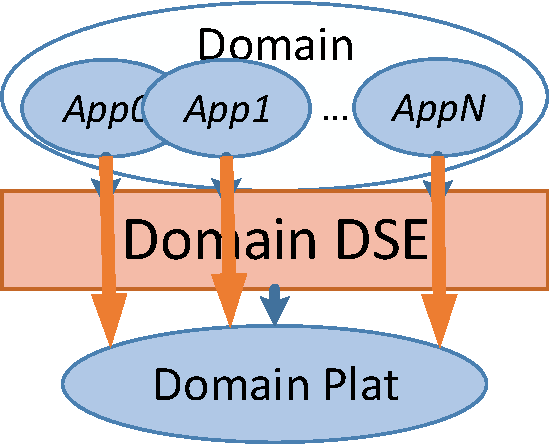
\includegraphics[width=.28\linewidth]{fig/pDomainP.pdf}\label{fig:DomainP}}
		\hfill
		\subfloat[OOP]{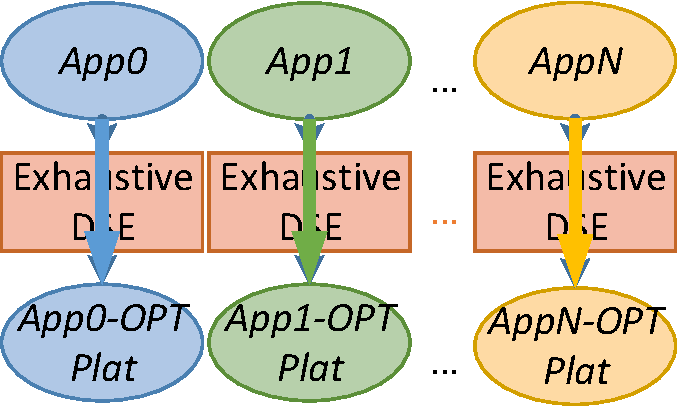
\includegraphics[width=.32\linewidth]{fig/pOOP.pdf}\label{fig:OOP}}
		\hfill
		\subfloat[FOP]{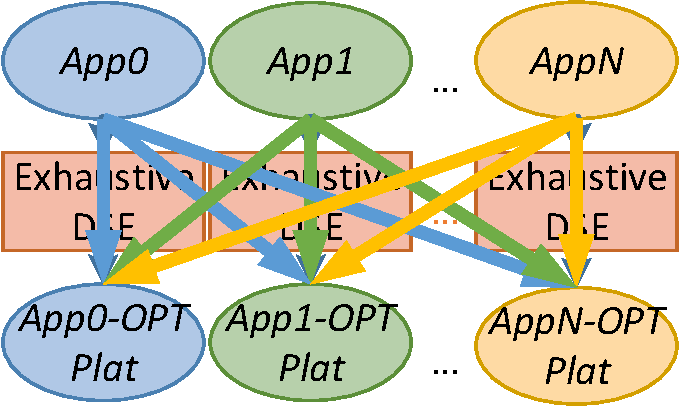
\includegraphics[width=.32\linewidth]{fig/pFOP.pdf}\label{fig:FOP}}
	%\vspace{-5pt}
	\caption{Experiments Settings}
	%\vspace{-4pt}
\end{figure}



We evaluate two domain types. The \textbf{OpenVX} domain (computer vision) has 35 function types and contains 40 applications from Intel \cite{Intel} and AMD \cite{AMD}, abstracted into data flow models. The \textbf{synthetic} domain is generated with 50 function types, containing 100 applications with a balance between processing and communication. 
%Performance is evaluated on automatically generated virtual platforms (SCE\cite{domer2008system}) capturing the abstract data flow model (SDF3\cite{stuijk2006sdf}) and architecture resources. 
The target platform contains a processor with N ACCs. Communication occurs on a 3R3W layer bus. The processing speedup on ACCs should be variable for different FTs, which could be implemented in different models, e.g. roofline model. For simplification, this paper just assumes ACC processing is 20x faster than SW. ACCs can communicate directly with each other~\cite{teimouri2016improving}.

\subsection{Domain Throughput Comparison}
\label{sec:resTh}

To gain a first global view, \figref{fig:th} plots the throughput improvement of the two domains over increasing HW budget.

%Graph is Average Throughput Improvement
\begin{figure}[htb]
	%\vspace{-10pt}
	\centering
		\subfloat[OpenVX Domain]{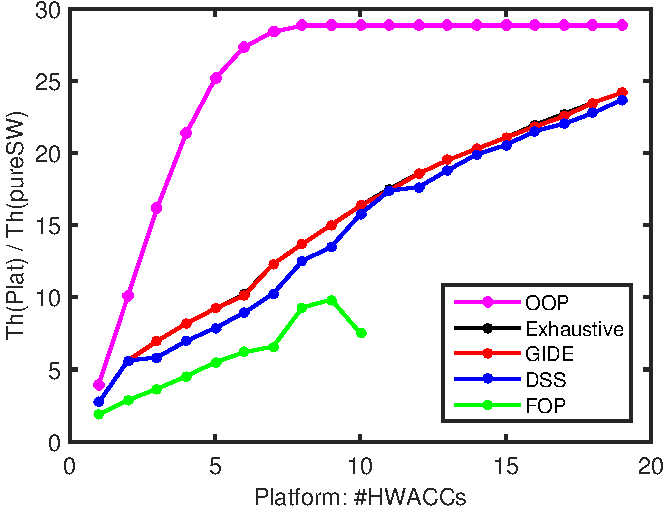
\includegraphics[width=.48\linewidth]{fig/prThOpenVX.pdf}\label{fig:thOpenVX}}
		\hfill
		\subfloat[Synthetic Domain]{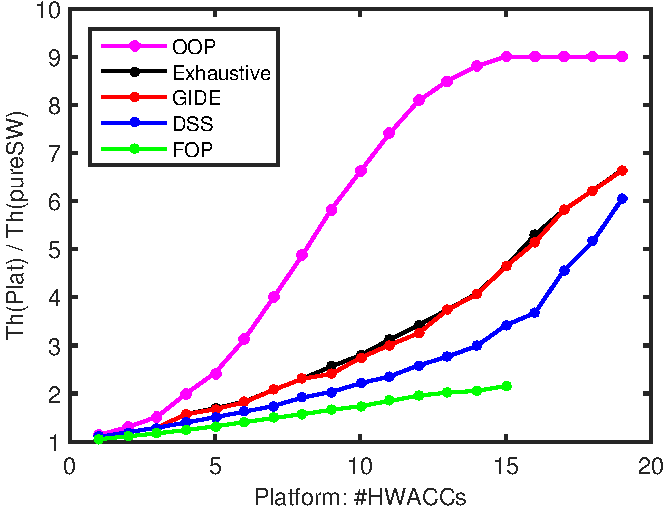
\includegraphics[width=.48\linewidth]{fig/prThSyn.pdf}\label{fig:thSyn}}
	%\vspace{-5pt}
	\caption{Average throughput improvement}
	\label{fig:th}
	%\vspace{-4pt}
\end{figure}

\textbf{OOP} yields highest (but unrealistic) throughput, see \figref{fig:thOpenVX}, assuming that each application were to execute on its own OPT. This indicates the acceleration potential. It saturates with budget $N$=10, when each application has enough accelerators. However, considering a single platform for all applications, \textbf{Exhaustive} indicates the optimum. It linearly increases with $N$ closing the gap to OOP, indicating that the additional area is well invested. \textbf{\ga} (actually \gah) almost achieves domain optimal, tracking Exhaustive. The greedy \textbf{DSS} is measurably below optimum but the gap narrows with budget. Exploring at application scope incurs dramatic penalties as indicated with \textbf{FOP} on the bottom.
FOP plateaus with 10 ACCs as already all possible ACCs have been selected for each application and it cannot outside this application to accelerate.
Comparing against FOP, \ga and DSS have 74.85\% and 58.02\% higher throughput ($N$\textless=10).

The synthetic domain, \figref{fig:thSyn}, exhibits similar trends. OOP and FOP saturate later $N$=15 due to the larger domain (more function types). Given larger domain, the gap between DSS and GA is increased. As the synthetic domain has a larger design space, the DSE performance has more impact on the results. Here, \ga and DSS have a 48.09\% and 23.60\% higher throughput ($N$\textless=15).

In order to better delineate DSE performance, we define the metric \textbf{average throughput achievement}. It scales the throughput improvement of a DSE generated platform over the throughput improvement of the domain optimal platform (i.e. Exhaustive) of the same budget. An throughput achievement of 1 thus indicates the optimum. \figref{res:pa} graphs the achievements.

%Graph is Performance Achievement
\begin{figure}[htbp]
	%\vspace{-10pt}
	\centering
		\subfloat[OpenVX Domain]{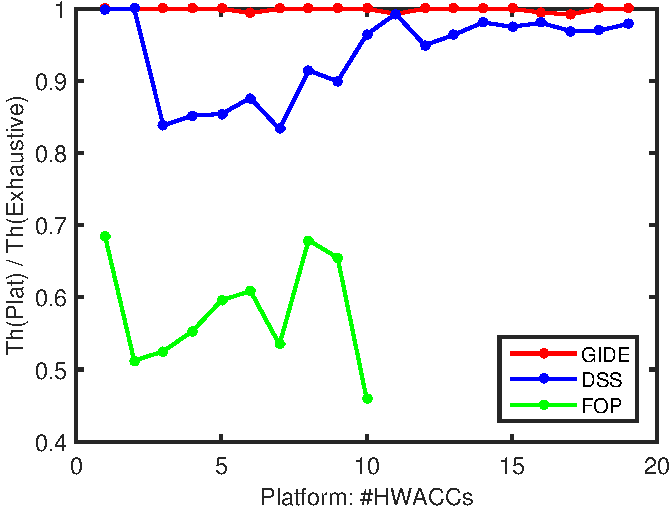
\includegraphics[width=.48\linewidth]{fig/prPAOpenVX.pdf}\label{fig:paOpenVX}}
		\hfill
		\subfloat[Synthetic Domain]{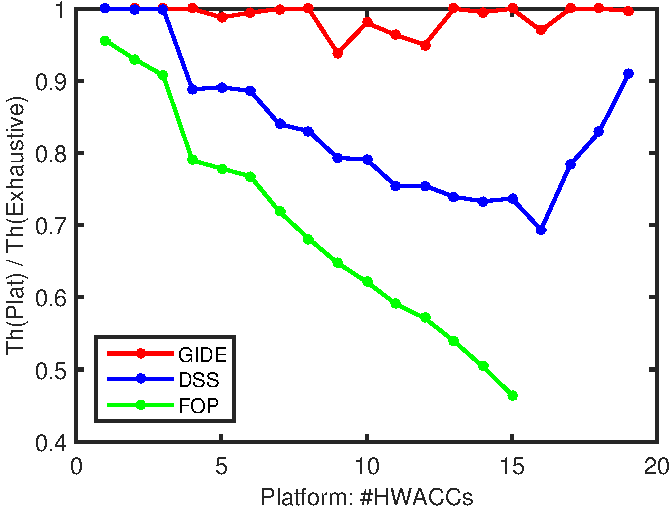
\includegraphics[width=.48\linewidth]{fig/prPASyn.pdf}\label{fig:paSyn}}
	%\vspace{-8pt}
	\caption{Average Throughput Achievement}
	\label{res:pa}
	%\vspace{-4pt}
\end{figure}

In \figref{fig:paOpenVX}, \ga achieves close to the optimum, with 99.87\% on average across all budgets for the OpenVX domain. DSS achieves less with 93.65\% and is not as stable. FOP has a large gap with only 58.07\%.

Considering the larger synthetic domain, \figref{fig:paSyn} shows even more differentiation. GA, DSS, FOP achieve 98.84\%, 83.45\% and 69.81\%, respectively. The gap between DSS and GA is more pronounced and largest gap shifts from $N$=7 in OpenVX to $N$=16 in synthetic domain. Beyond that point, DSE performance is not as critical as with a higher HW budget the margins between the ACCs selection become smaller, thus selecting a sub-optimal ACC has a lower penalty.



\subsection{\ga Variant Analysis}
\label{sec:resMutation}

In order to understand the DSE contributions of individual \ga aspects, we analyze the variants with respect to throughput achievement and exploration time of the synthetic domain, see \figref{fig:dse:tr}.

%Graph show the GA+LS(Hybrid) is the best.
\begin{figure}[h]
	\centering
	%\vspace{-10pt}
	\subfloat[Throughput Achievement]{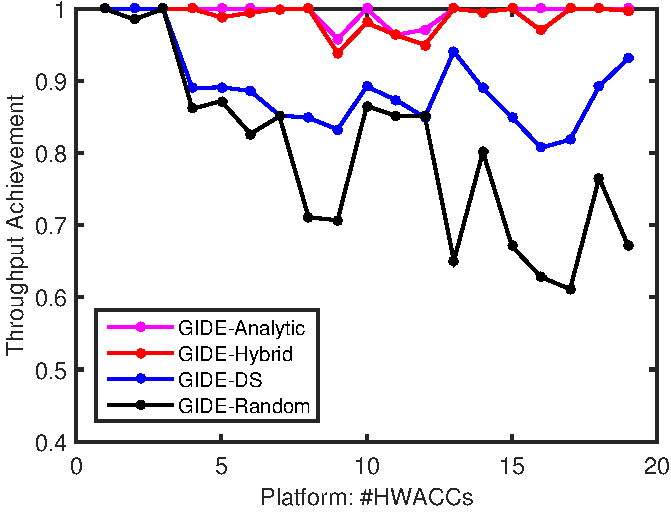
\includegraphics[width=.48\linewidth]{fig/prPAGASyn.pdf}\label{fig:paGASyn}}
	\hfill
	\subfloat[Exploration Time]{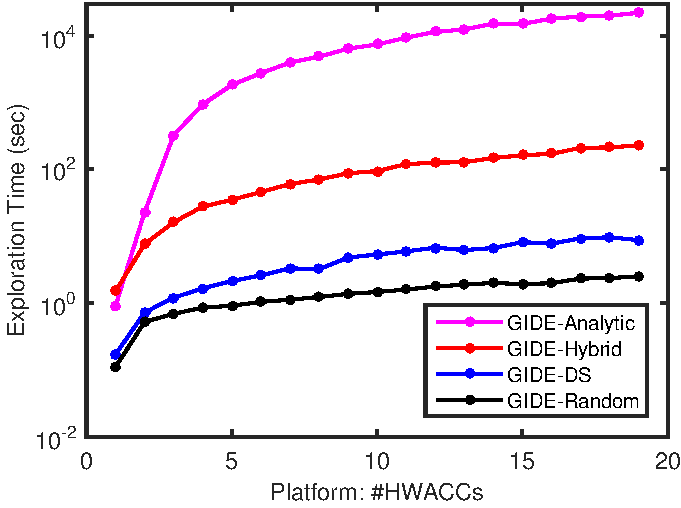
\includegraphics[width=.48\linewidth]{fig/prTimeGASyn.pdf}\label{fig:timeGASyn}}
	%\vspace{-5pt}
	\caption{Comparing \ga Variants (Synthetic)}
	\label{fig:dse:tr}
	%\vspace{-10pt}
\end{figure}




\gah and \gaana exhibit very similar achievements, see Fig.~\ref{fig:paGASyn}. They are close to optimal which is 99.41\% and 98.84\%, respectively, increasing the confidence in selecting the hybrid approach. Conversely, \gads is hampered with the DS accuracy in the guided local, only achieving 89.20\%. The inaccuracy of DS can lead to getting the local search being stuck at an invalid local optimum. \garand has the lowest achievement with 79.90\% on average over budget.

Looking at exploration time, \figref{fig:timeGASyn}, \garand is the fastest with 2 seconds. \gads, \gah and \gaana are around 5x, 100x, 10000x slower than random mutation. 
%
Comparing both achievement and exploration time sets out \gah as the best choice being 100x faster than \gaana while still achieving close to optimum results. Its two step of initial pruning with DS followed by more detailed analytic evaluation clearly sets it apart.  


\begingroup
\setlength{\columnsep}{8pt}%

\begin{wrapfigure}{l}{0.5\linewidth}
	%\vspace{-6pt}
	\begin{center}
		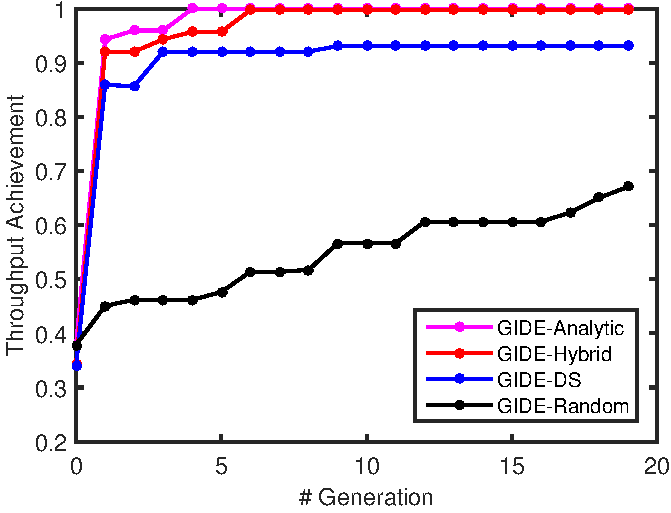
\includegraphics[width=\linewidth]{fig/prPAGenSyn.pdf}
	\end{center}
	%\vspace{-8pt}
	\caption{Improvement per Generation}
	\label{fig:paGenSyn}
	%\vspace{-4pt}
\end{wrapfigure}


To gain more insight with exploration generations, \figref{fig:paGenSyn} explores the achievement for a constant budget of $N$=19 in the synthetic domain. \gaana is the fastest to reach the best solution in only 5 generations. \gah is only 2 generations behind. \gads although rapidly reaching 90\% in a few generations, it cannot improve much over the remaining generations as it is stuck in an inaccurate local maximum. \garand needs many more generations, but steadily improves over them. 

\endgroup
%\begin{figure}[h]
%	\centering
%		\subfloat[OpenVX Domain]{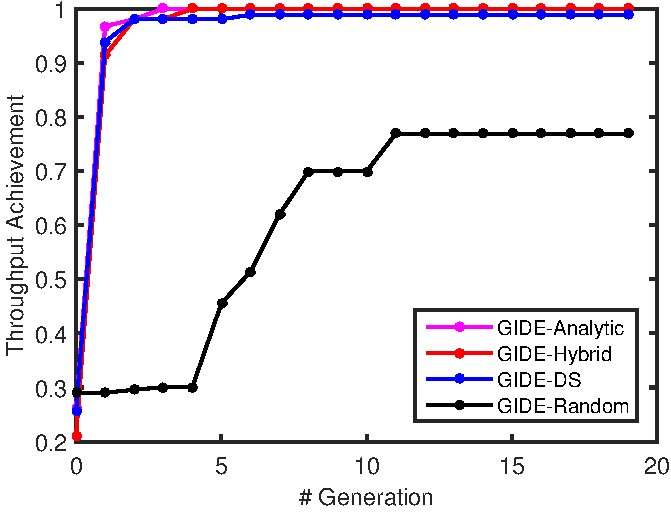
\includegraphics[width=.5\linewidth]{fig/prPAGenOpenVX.pdf}\label{fig:paGenOpenVX}}
%		\hfill
%		\subfloat[Synthetic Domain]{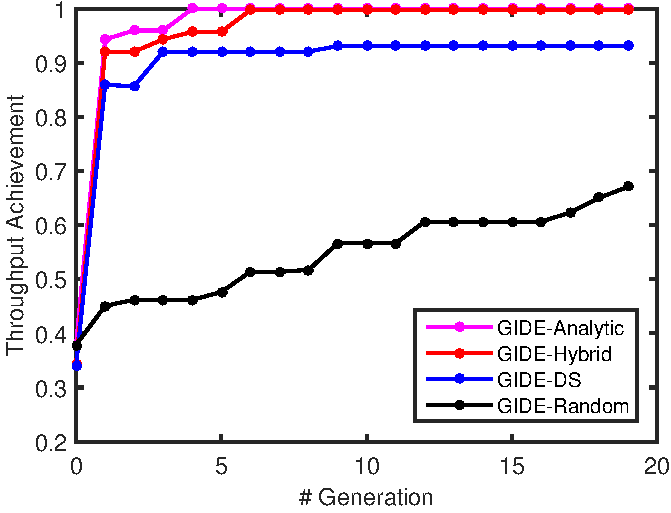
\includegraphics[width=.5\linewidth]{fig/prPAGenSyn.pdf}\label{fig:paGenSyn}}
%	\caption{Improvement per Generation}
%\end{figure}

%\begin{figure}[h]
%	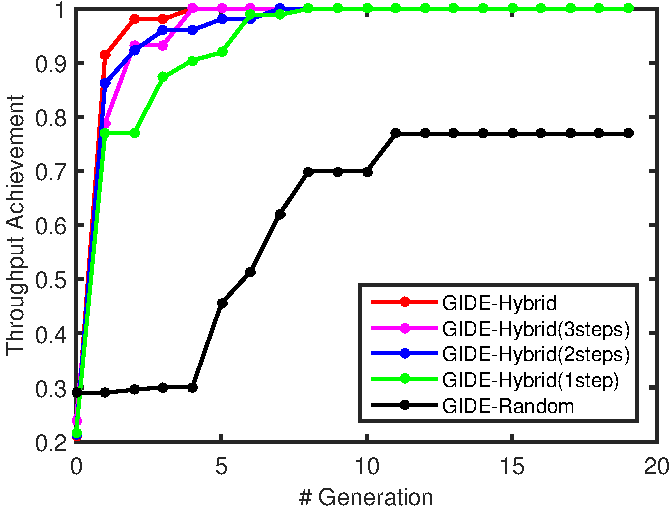
\includegraphics[width=.75\linewidth]{fig/prStepLimit.pdf}
%	\caption{OpenVX: GA limit number steps of local search}
%	\label{fig:stepLimit}
%\end{figure}



Our measurements demonstrate that the guided local search is highly efficient. To gain even further insight we measure
the average number of search steps and the effect of artificially limiting the search depth when exploring the OpenVX domain.
%Graph to show the step number of local search is acceptable. (Graph is need to re-draw)
\begin{figure}[h]
	\centering
		\subfloat[Average \# of Steps]{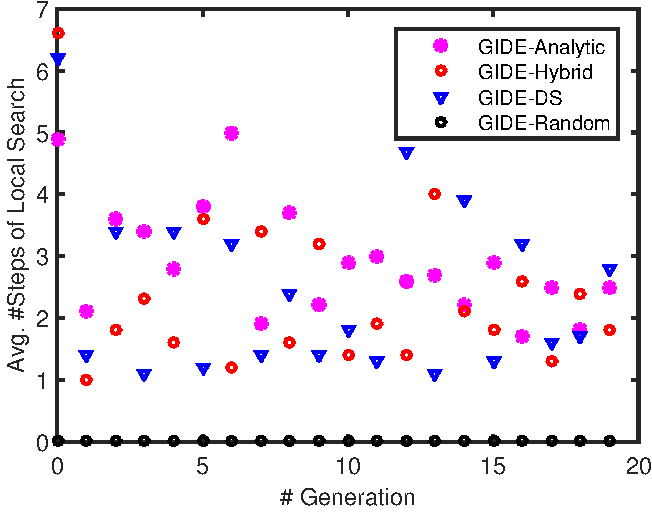
\includegraphics[width=.48\linewidth]{fig/prStepAve.pdf}\label{fig:stepAve}}
		\hfill
		\subfloat[Limit Steps of Local Search]{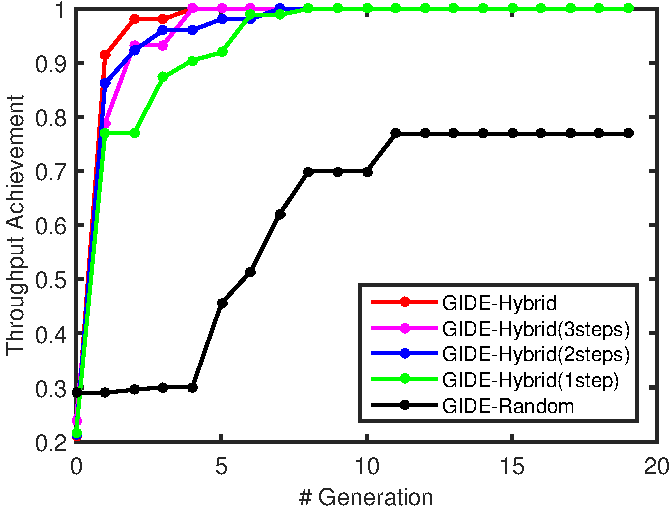
\includegraphics[width=.48\linewidth]{fig/prStepLimit.pdf}\label{fig:stepLimit}}
	\caption{Local Search Steps}
	\label{fig:step}
\end{figure}


%\begingroup
%\setlength{\columnsep}{8pt}%

%\begin{wrapfigure}{l}{0.5\linewidth}
	%\vspace{-6pt}
%	\begin{center}
%		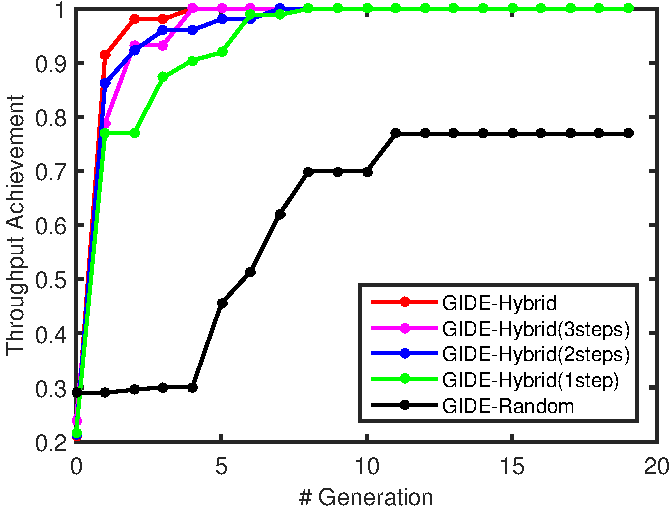
\includegraphics[width=\linewidth]{fig/prStepLimit.pdf}
%	\end{center}
	%\vspace{-8pt}
%	\caption{Limit Steps of Local Search}
%	\label{fig:stepLimit}
	%\vspace{-4pt}
%\end{wrapfigure}

\newtext{In} \figref{fig:stepAve}, \gaana, \gah and \gads have all a very low number of average steps across generations with, 2.91, 2.37, and 2.41 respectively. Even its maximum is low with 10 (\gaana), and 8 (for both \gah and \gads). The low number of steps can be explained with the exhaustive search of the neighborhood. Sparser sampling approaches, conversely, would need more steps. Limiting the maximum number of search steps only minimally impacts search performance as shown in \figref{fig:stepLimit} for the OpenVX domain. Although limiting to 3 steps, \gah still finds the optimum in 4 steps in this example. Further limiting the number of steps translates into requiring more generations (+3 with 2 steps, +4 with 1 step) nonetheless the same solutions are still reached. Due to the speed of DS evaluation, we do not limit the number of steps. 

%\endgroup

%GA summary - GS CUT
% GA with different mutations Trade-off between throughput achievement and exploration time.
%Summarizing the detailed results confirms our selection of \gah as the most suitable approach providing both s
%Random and DSS have the fast exploration, but the performance is bad.
%The Analytical and Hybrid has the almost highest performance.
%Hybrid is 100x faster than analytical evaluation.
%GA-Hybrid is the best choice for domain DSE for most cases.
%However, if want to get the highest performance design, and do not care about the exploring time, the GA-analytical could be considered.
\subsection{Scalability with Increasing Domain Size}
\label{sec:res:size}

%Domain Analyzer Time
\newtext{The exploration time to identify a domain-specific platform using our approach consists of two parts: domain analysis and design exploration. The initial domain analysis is fast: analyzing the synthetic domain with 100 apps (with up to 12 nodes each) on Intel i5-3450 with 3.10GHz takes 22.1s. Since the initial domain analysis only executes only once, this section mainly focuses on the scalability of domain exploration.} 

%Graph to show the scalability of our graph
Exploration time is correlated to the size of the domain, more specifically: the number of function types. \figref{fig:scale} analyzes the exploration time as well as the achievement over number of function types to measure scalability. 

\begin{figure}[h]
	%\vspace{-5pt}
	\centering
		%\subfloat[FT=50, diff HW budget]{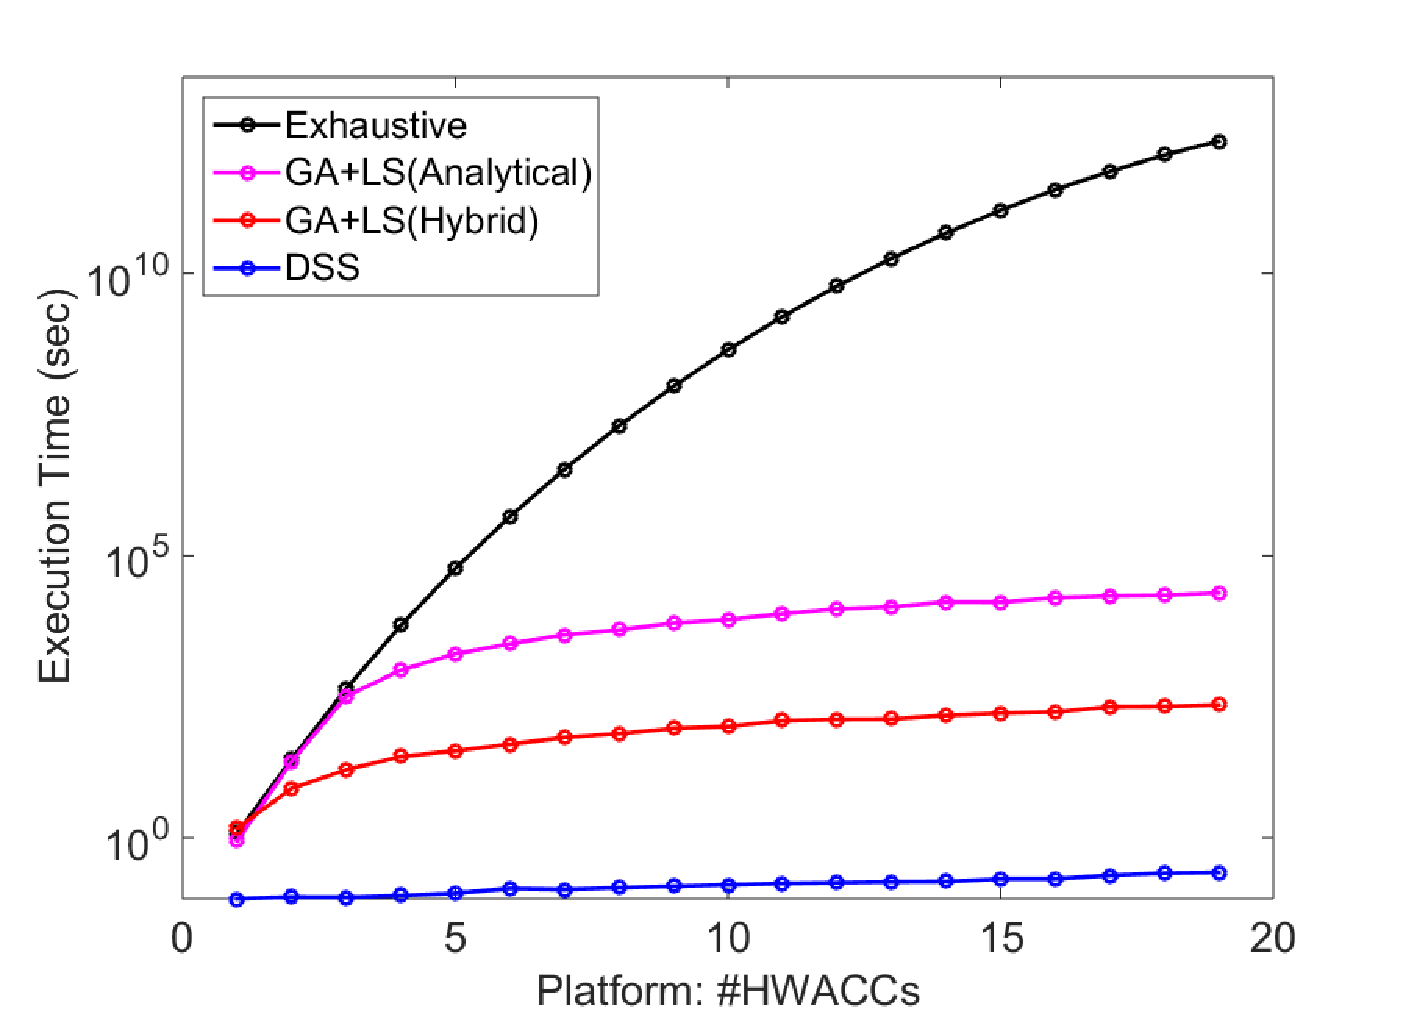
\includegraphics[width=.5\linewidth]{fig/prTimeHW.pdf}\label{fig:timeHW}}
		\subfloat[Exploration Time]{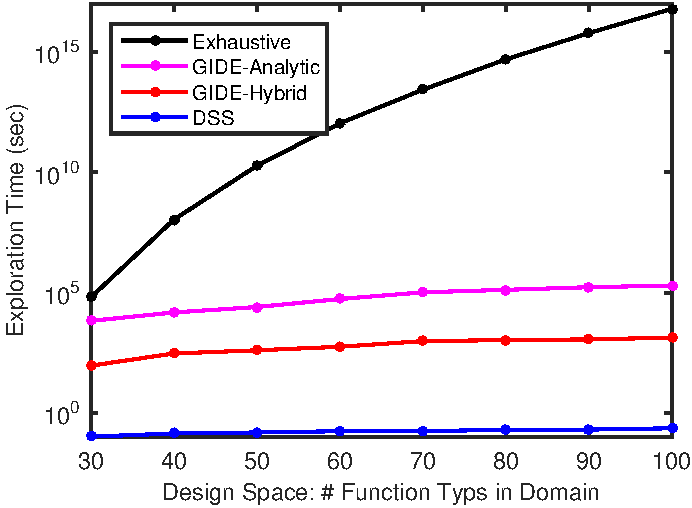
\includegraphics[width=.5\linewidth]{fig/prTimeSpace.pdf}\label{fig:timeSpace}}
		\hfill
		\subfloat[Relative Throughput]{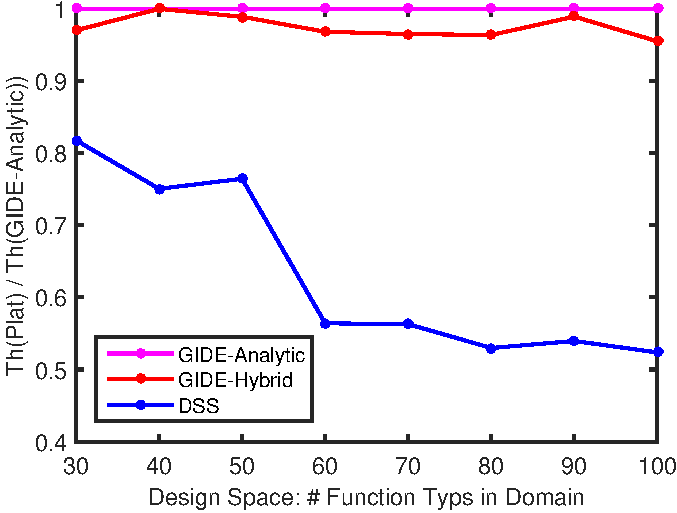
\includegraphics[width=.5\linewidth]{fig/prPASpace.pdf}\label{fig:paSpace}}
	%\vspace{-4pt}
	\caption{Scalability with Domain Size}
	\label{fig:scale}
	%\vspace{-8pt}
\end{figure}

\figref{fig:timeSpace} shows that with increasing design space, DSS and \ga scale well only slowdown linearly. The orders of magnitude comparisons hold with these approaches across size. Conversely, the Exhaustive search exponentially increases exploration time (estimation only). The benefits are most predominant with the largest domain (FT=100). Here, \gah is $4.6*10^{13}$ times faster than exhaustive.

Fig.~\ref{fig:paSpace} illustrates the stability of results over increasing domain size. However, obtaining the domain optimal platform is infeasible due to exorbitant long exploration time ($3*10^8$ years, FT=100). As an approximation, \figref{fig:paSpace} shows relative throughput compared to \gaana. Even over large domains \gah scales very well and its results remain close to \gaana with 97.51\% on average. Conversely, the limitations of DSS become more pronounced as domain size increases (63.16\%).

%Performance over increasing domain size. The first graph should be changed to performance versus time.
%\begin{figure}[H]
%	\centering
%		\subfloat[Relative Throughput]{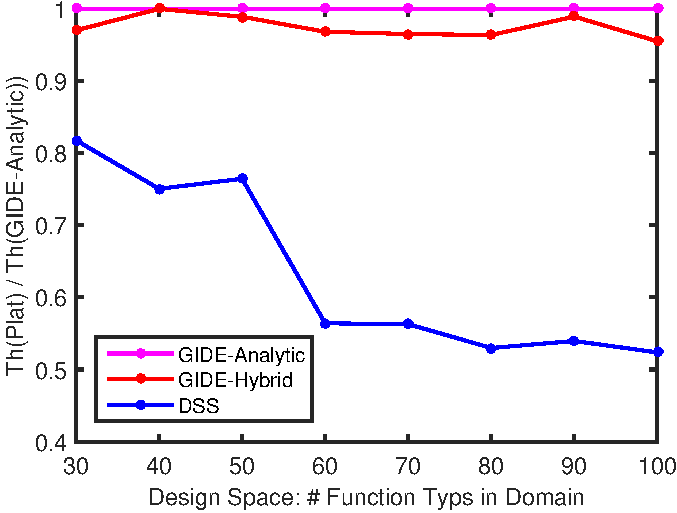
\includegraphics[width=.5\linewidth]{fig/prPASpace.pdf}\label{fig:paSpace}}
%		\hfill
%		\subfloat[Performance vs Time]{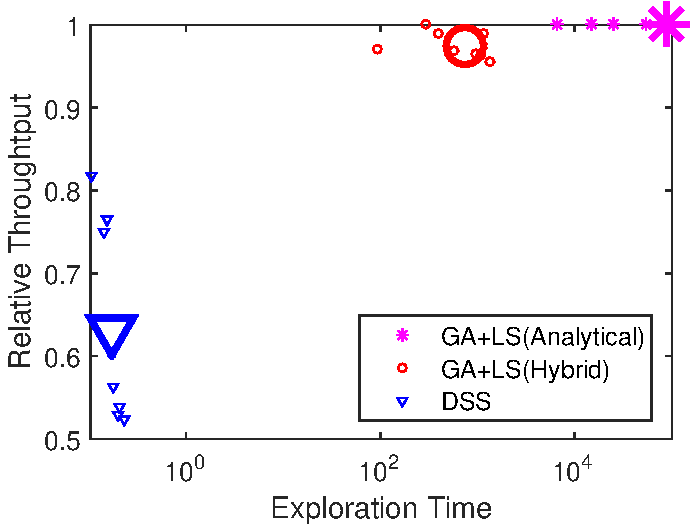
\includegraphics[width=.5\linewidth]{fig/prPATimeSpace.pdf}\label{fig:paTimeSpace}}
%	\caption{Synthetic Domain: HW=19, with diff design space}
%\end{figure}

%Fig.~\ref{fig:paTimeSpace} trade-off. GA Hybrid could achieve high performance, with less exploring time compared with GA-analytical. Although the DSS is much faster than other two algorithm, it could get the good domain platform.
\subsection{Effects of Unknown Applications}
\label{sec:res:unknown}

The quality of a domain platform is also expressed in how well it supports applications unknown at design time. We explore the effect for the OpenVX domain. For this, the DSE is performed with N-1 domain applications. Throughput measurements, conversely, are performed using \newtext{the unknown application.} The process is repeated N times and results averaged. \figref{fig:unknown} reports the results.

\begin{figure}[h]
	%\vspace{-5pt}
	\centering
		\subfloat[Average Throughput Improvement]{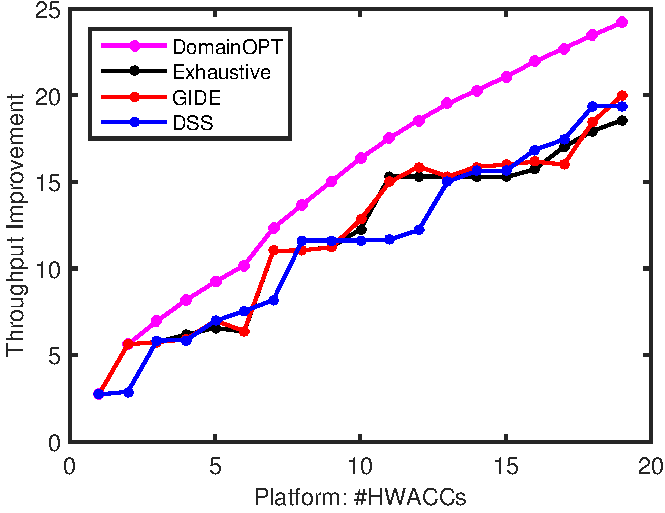
\includegraphics[width=.5\linewidth]{fig/prUnknowTh.pdf}\label{fig:unknownTh}}
		\hfill
		\subfloat[\newtext{Cumulative Performance Loss} (HW=8)]{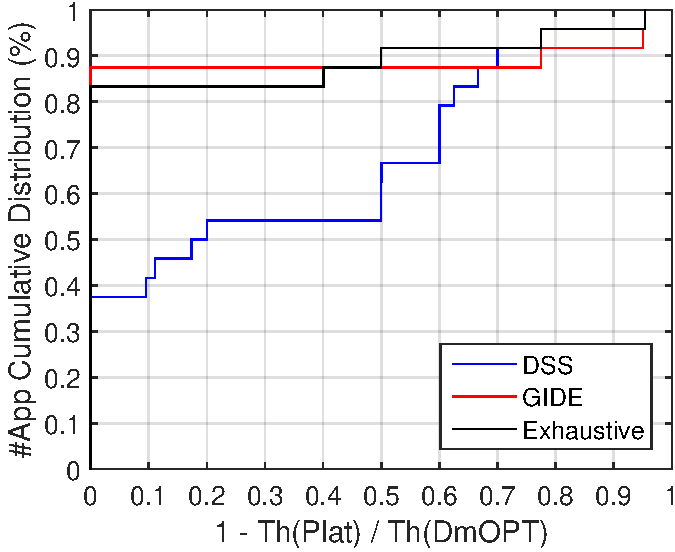
\includegraphics[width=.47\linewidth]{fig/prUnknowCD.pdf}\label{fig:unknownCD}}
	%\vspace{-8pt}
	\caption{N-1 Training, 1 Evaluation Rotating (OpenVX)}
	\label{fig:unknown}
	%\vspace{-6pt}
\end{figure}

As \figref{fig:unknownTh} shows that even the exhaustive search exhibits a significant loss over \textbf{DomainOPT} which is the oracle solution knowing all applications at design time. Comparing DSE approaches is inconsistent, as each is at least once the best due to averaging.  

\figref{fig:unknownCD} reveals much more insight showing the cumulative distribution of application throughput achievement (over DomainOPT) for a budget of 8 (where DSS had highest average improvement). 
Exhaustive and \ga show a much better distribution than DSS. In Exhaustive and \ga more than 80\% applications could achieve highest throughput. 
The reason of higher DSS average, is that DSS fully accelerate some applications which have a very high individual throughput improvement.  However, for a large size of low throughput improvement, the DSS can not accelerate it. 


%\begin{figure}[H]
%	\centering
%	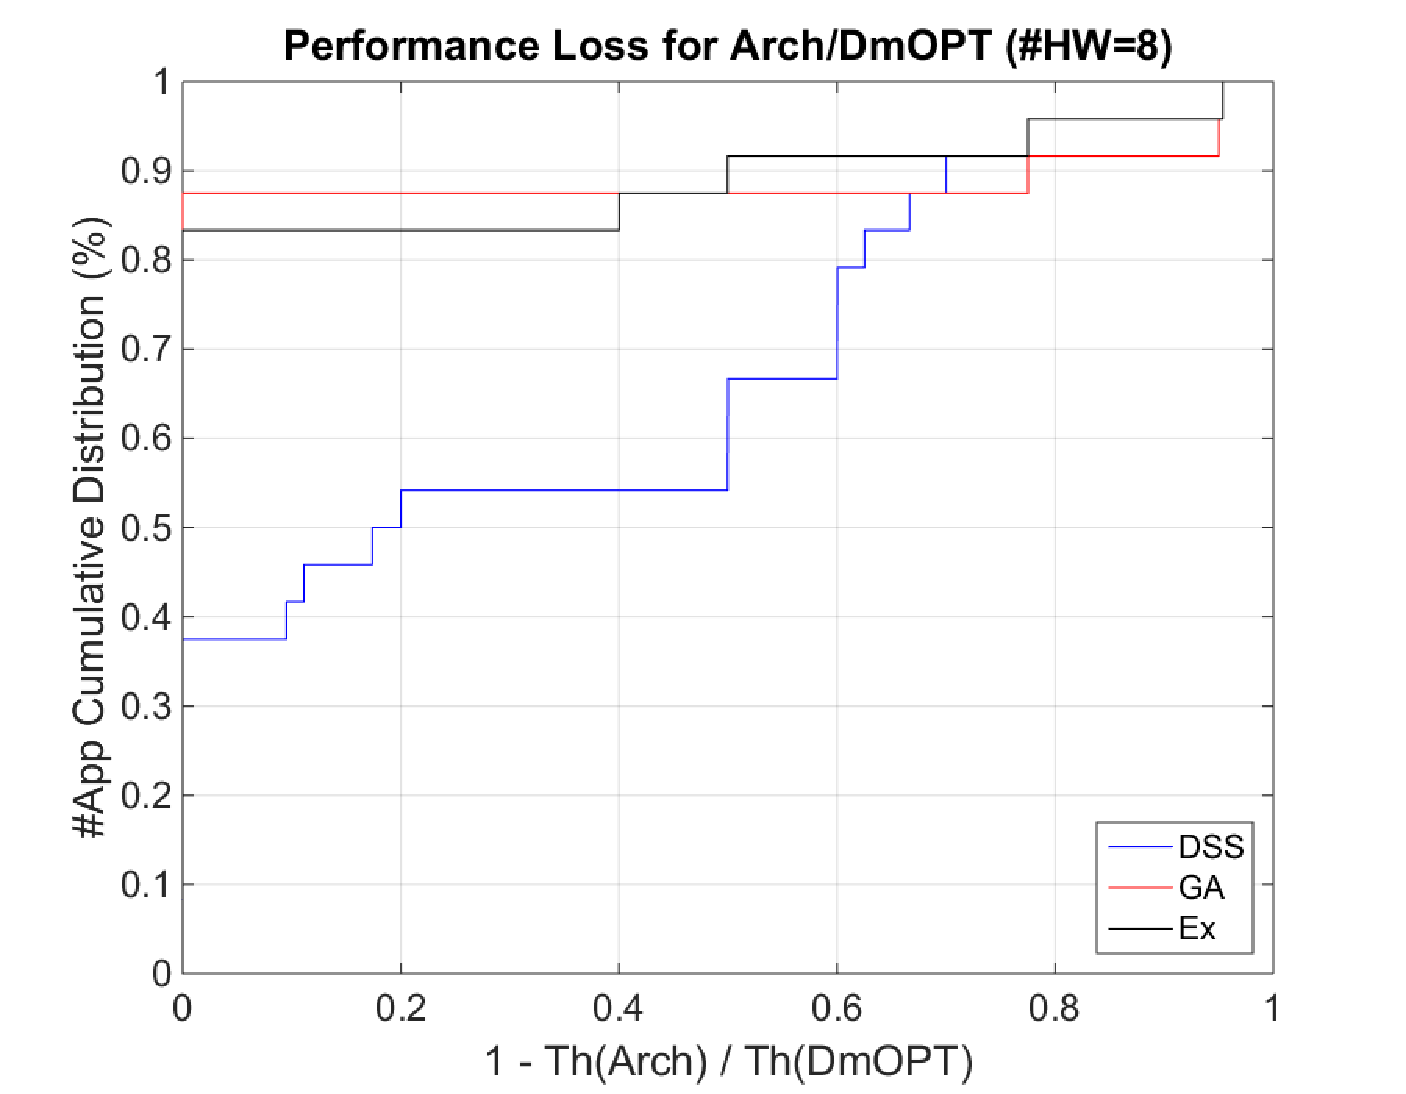
\includegraphics[width=.7\linewidth]{fig/resPerfLoss.pdf}
%	\caption{OpenVX: Throughput Loss Cumulative Distribution}
%	\label{fig:resOpenVXLoss}
%\end{figure}

%\vspace{-5pt}
\subsection{Generalization}
\label{sec:generalization}
%\vspace{-3pt}

Our analysis is best summarized as the DSE trade-off between exploration time and achieved performance. \figref{fig:paTime} quantifies the trade-off for OpenVX and synthetic domain. 


\begin{figure}[H]
	%\vspace{-5pt}
	\centering
		\subfloat[OpenVX Domain]{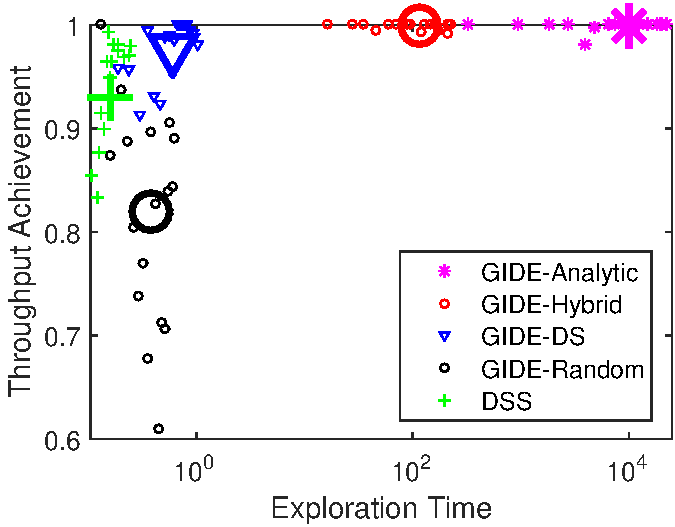
\includegraphics[width=.5\linewidth]{fig/prPATimeOpenVX.pdf}\label{fig:paTimeOpenVX}}
		\hfill
		\subfloat[Synthetic Domain]{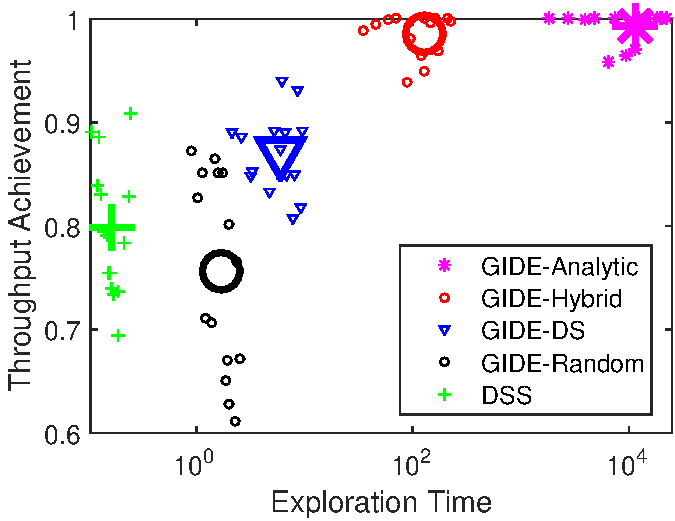
\includegraphics[width=.5\linewidth]{fig/prPATimeHWSyn.pdf}\label{fig:paTimeHWSyn}}
		%\vspace{-6pt}
	\caption{Design Exploration trade-off}
	\label{fig:paTime}
		%\vspace{-6pt}
\end{figure}

As domain size increases the trade off becomes more pronounced, i.e. it is more visible for the synthetic domain \figref{fig:paTimeHWSyn}. 
DSS achieves the fastest results but with low accuracy. \garand is similar in accuracy but much slower. DSS outperforms \garand as it uses domain features to guide the exploration. \gads produces designs with limited performance as it is limited by DS accuracy. Both \gah and \gaana approach optimal performance, while \gah is 100x faster. This makes \gah the preferred approach for DS-DSE.


\section{Conclusion}

\label{sec:conclusion}
\newtext{This paper introduced a Domain-specific Design Space Exploration (DS-DSE) methodology to broaden the scope of existing DSE from individual apps in isolation to a whole domain. This paper lays the foundations by defining a domain and quantifiable features (metrics) that can guide exploration. The features take both behavioral (processing) and structural (communication) aspects into account, as well as consider the distribution over the domain.} 

\newtext{Based on these definitions, the paper has introduced the Dynamic Score Selection (DSS) and GenetIc Domain Exploration (GIDE) algorithms for domain exploration. These algorithms maximize domain throughput creates a domain-specific architecture that has more flexibility to execute domain applications. DSS uses Domain Score (DS) to estimate platform performance in the domain level.} \ga employs a guided local search with hybrid analytical and DS evaluation models to enhance the domain exploration efficiency. \newtext{Our experimental results (Synthetic and OpenVX domains) demonstrate that} DSS achieves 23.60\%-58.02\%, and \ga achieves 48.09\%-74.85\% performance improvement compared to application-specific FOP platform. \ga almost achieves domain optimal throughput (97.6\% to 99.8\%), with around $1*10^{13}$ faster compared with exhaustive search.

%This paper introduced a novel algorithm, GenetIc Domain Exploration (GIDE), for rapid Domain-specific Design Space Exploration (DS-DSE). The significance of \ga is broadening the scope of the genetic algorithm from a single application to a domain of applications. It employs a guided local search with hybrid analytical and domain score evaluation models to enhance the domain exploration efficiency. Our experimental results show that \ga almost achieves domain optimal throughput (97.6\% to 99.8\%), with around $1*10^{13}$ faster compared with exhaustive search. \ga also achieves 10.65\% to 19.81\% and 48.09\% to 74.85\% higher domain throughput  compared against domain-specific DSS \cite{zhang100ds} and application-specific FOP platforms.


%\vspace{-8pt}
\section{Preliminaries}
\label{sec:Pre}

To set the stage for our proposed domain DSE approach (GIDE), this sections introduces our assumptions / formalizations about the target platform and capturing domain applications.

\input{tex/platform}
\section{Domain Formalization}
\label{sec:Domain}

The foundation of any systematic approach for domain-specific-DSE is the formalization of a domain and its features (metrics) to quantitatively reason about the domain. This section defines the domain scope and its features (metrics). They capture the behavioral and structural features of a domain showing what functions are commonly used and how they are composed. Defining these features and metrics lays the foundation for automatic domain analysis and exploration.

\subsection{Domain Definition}
\label{sub:dmDefine}
Domain is a set of applications, which share common functions and common patterns\cite{kang1990feature}. To allow reasoning about the domain\footnote{Defining the scope of a domain, i.e. assessing domain membership, is an additional research topic.}, we formally define it as a set of graphs.
%Current definitions of domain include a set of applications which share a set of common capabilities and data \cite{kang1990feature}, a class of applications, with a component library, which contains reusable chunks of domain expertise \cite{tracz1995dssa}. Following this definition, we define a domain as a set of applications, which share common functions and common patterns. To allow reasoning about the domain\footnote{Defining the scope of a domain, i.e. assessing domain membership, is an additional research topic.}, we formally define it as a set of graphs.
%\vspace{-5pt}
\begin{equation}
\begin{split}
\label{eq:domain}
	&G = \{g_{0}, g_{1}, ..., g_{N}\}, \quad g_{i} = (A, E)\\
	&A = \{a_{0}, a_{1}, ..., a_{n}\}, \quad E = \{e_{0}, e_{1}, ..., e_{m}\}\\
	&a_{i} (t, d_{P}), \quad e_{i} ((a_{src}, a_{dst}), d_{C})
\end{split}
\end{equation}
%\endgroup
%\vspace{-10pt}

In Eq.~\eqref{eq:domain}, domain $G$ is a set of streaming applications ($g_{0}$ .. $g_{N}$), each captured as a dataflow graph \cite{stuijk2006sdf}. Each application $g_i$ contains a set $A$ of processing actors ($a_0$ .. $a_n$) and a set of $E$ edges ($e_0$ .. $e_m$) representing the communication between actors. Each actor $a_i$ is an instance of a function type $t$ with an instance-specific processing demand $d_{P}$ (\# of operations). Multiple instances of the same function type $t$ may exist within and across applications within the domain. Each edge $e_i$ is the directed communication between its $a_{src}$ and $a_{dst}$ with a communication demand of $d_{C}$ as a measure of the transferred volume (bytes). E.g., in application $g0$ of Fig.~\ref{fig:Apps}, the first actor $A0$ is an instance of $t_{A}$ and its $d_{P} = 350$, and the edge between $A0$ and $B0$ contains $d_{C} = 50$. 

\begin{table}[h]
  \begin{minipage}[b]{0.35\linewidth}
    \centering
    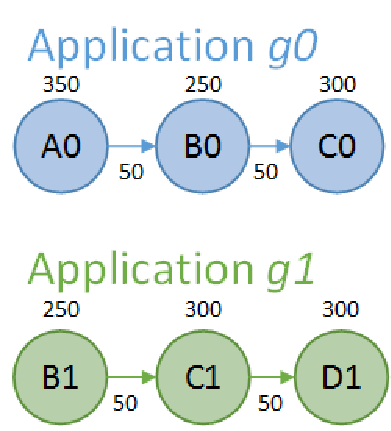
\includegraphics[width=0.9\linewidth]{fig/Apps.pdf}
    \captionof{figure}{Example: Domain Applications}
    \label{fig:Apps}
  \end{minipage}
	 \hfill
  \begin{varwidth}[b]{0.6\linewidth}
    \centering
    \begin{tabular}{l r r r}
      \toprule
      Composition & $P$ & $D_{P}$ & $D_{C}$ \\
      \midrule
      $\{t_A\}$ & 50\% & 350 & -- \\
      $\{t_B\}$ & 100\% & 500 & -- \\
      $\{t_C\}$ & 100\% & 600 & -- \\
      $\{t_D\}$ & 50\% & 300 & -- \\
			\hline
			$\{t_A,t_B\}$ & 50\% & -- & 50 \\
			$\{t_B,t_C\}$ & 100\% & -- & 100 \\
			$\{t_C,t_D\}$ & 50\% & -- & 50 \\
			\hline
			$\{t_A,t_B,t_C\}$ & 50\% & -- & -- \\
			$\{t_B,t_C,t_D\}$ & 50\% & -- & -- \\			
      \bottomrule
    \end{tabular}
    \caption{Example: Domain Features}
    \label{tab:egFeature}
  \end{varwidth}
\end{table}
\subsection{Domain Features}
\label{sec:features}
Domain features lay the foundation for automatic exploration. It is essential to capture behavioral similarity to assess processing needs, and structural similarities to assess communication / topology requirements. Aligned with the domain definition, we identify commonly used functions and function patterns. We express common functions as the function types of actors that repeat within and across applications. Function patterns are repeating compositions these function types (i.e. identical subgraphs). Different lengths of compositions are considered. For example, application $g0$ in Fig.~\ref{fig:Apps}, has three, two and one composition of a degree one, two and three, respectively. The function type composition $\{t_{B}, t_{C}\}$ (which is of degree 2) appears in application $g0$ (actors $B0$,$C0$) and $g1$ ($B1$,$C1$). \tabref{tab:egFeature} lists the compositions of the domain.

%removed the detour of instances. Directly explained it as types. no addl. formula neede
%The definitions of actor composition $c$ and function type composition $C$ are given in Eq.~\ref{eq:comps}.   
%
%\vspace{-10pt}
%%\begingroup\makeatletter\def\f@size{9}\check@mathfonts
%\begin{equation}
%\begin{split}
%\label{eq:comps}
	%c = \{a_j, a_k,...\}, \quad C = \{t_J, t_K,...\}\\
%\end{split}
%\end{equation}
%%\endgroup
%%\vspace{-10pt}

A composition of degree one ($\left\vert{C}\right\vert = 1$) contains a single function type. All compositions $\left\vert{C}\right\vert = 1$, represent the function types shared across the domain. Since compositions $C$ can capture both common functions (behavioral similarity) and function patterns (structural similarity), this paper chooses function type compositions $C$ to express domain features. In addition to the subgraph of function types, we focus on three aspects to characterize compositions: probability of appearance, processing demand and communication demand. 

Compositions that appear more often across applications are more important for the domain than infrequent compositions. To quantify the importance, we define appearance probability $P$ as per Eq.~\eqref{eq:p}. 

%\vspace{-10pt}
\begin{equation}
\begin{split}
\label{eq:p}
P(C_i) = (\sum_{g_j \in G} \left\vert \{ Instance(C_i) \in g_j \} \right\vert) / \left\vert{G}\right\vert \\
%	P(C) = \left\vert{ \{g \vert c \in g, c \in C \} }\right\vert / \left\vert{G}\right\vert \\
\end{split}
\end{equation}


$P$ is probability that an instance of composition $C_i$ appears in a domain application. The composition $\{t_{B}, t_{C}\}$ in Fig.~\ref{fig:Apps} and Table~\ref{tab:egFeature} appears in all applications ($P$ = 100\%). Whereas $\{t_A, t_B\}$ and $\{t_C, t_D\}$ each appear only in one ($P$ =50\%).  

A key challenge to enable domain DSE is how to identify processing and communication demands across applications which are necessary to guide resource allocation. However, considering each individual application is impractical. To obtain a domain-level view, we aggregate the demands for each composition as defined in Eq.~\eqref{eq:demand}.

%\vspace{-8pt}
\begin{equation}
\begin{split}
\label{eq:demand}
	&D_P(C_i=\{t_j\}) = \sum_{g_k \in G} \sum_{ a_l = Instance(t_j) \in g_k} a_l.d_P\\
	&D_C(C_i=\{t_i, t_j\}) = \sum_{g_k \in G} \sum_{e_l \in g_k, e_l=\{t_i,t_j\}} e_l.d_C
\end{split}
\end{equation}
%\vspace{-10pt}

%In general, DSE compares the processing workload $d_P$ among computing actors to decide which to accelerate and analyzes the communication $d_C$ between them to avoid data transfer. However, the individual $d_P$ and $d_C$ is a mess for DS-DSE. The DS-DSE needs the features in domain level to decide the partitioning of function types. 

The processing demand $D_P$ is calculated for each composition $C_i$ with a degree of one as the sum over all applications and all instances of the type $t_j$ (e.g. $D_P(t_B)$ = 500). Communication demand is computed for each pair of actor types (i.e. compositions of degree two). It is the sum of the communication demand for each edge of that type over all applications ($D_C(\{t_B, t_C\})$ = 100). 

%\vspace{-10pt}
\begin{equation}
\begin{split}
\label{eq:CS}
	&CS = \{C_{0}, C_{1}, ..., C_{z}\}\\
	&C_{i} (P, D_P, D_C)\\
\end{split}
\end{equation}
%\vspace{-10pt} 

In summary, the domin features are captured as a set of compositions, where each composition $C_i$ is defined by its appearance probability $P$, processing demand $D_{P}$ (for $\left\vert{C_i}\right\vert = 1$), and communication demand $D_{C}$ (for $\left\vert{C_i}\right\vert = 2$).
Table~\ref{tab:feature} shows the general view of the selected domain features. 

%GSTODO table is redundant in my view
\begin{table}[h]
	\caption{Domain Features}
	\label{tab:feature}
	\centering
	\begin{tabular}{p{0.06\linewidth}|p{0.22\linewidth}|p{0.15\linewidth}|p{0.15\linewidth}|p{0.18\linewidth}}
		\toprule
		\multicolumn{2}{c|}{Composition}& Appearance Probability& Processing Demand& Communication Demand\\
		\midrule
		\hline
		$C_{0}$&				$\{t_{A}\}$&								$P(C_{0})$&					$D_{P}(C_{0})$& --\\
		$C_{1}$& 				$\{t_{B}\}$&								$P(C_{1})$&					$D_{P}(C_{1})$& --\\
		$...$& 					$...$&									$...$&							$...$&	--\\
		$C_{x}$& 				$\{t_{N}\}$&								$P(C_{x})$&					$D_{P}(C_{x})$& --\\
		\hline
		$C_{x+1}$& 			$\{t_{A}, t_{B}\}$&					$P(C_{x+1})$&				--& $D_{C}(C_{x+1})$\\
		$C_{x+2}$& 			$\{t_{A}, t_{C}\}$&					$P(C_{x+2})$&				--& $D_{C}(C_{x+2})$\\
		$...$& 					$...$&									$...$&							--&			$...$\\
		$C_{y}$& 				$\{t_{I}, t_{N}\}$&					$P(C_{y})$&					--& $D_{C}(C_{y})$\\
		\hline
		$C_{y+1}$& 			$\{t_{A}, t_{B}, t_{C}\}$&		$P(C_{y+1})$&				--&	--\\
		$...$& 					$...$&									$...$&							--&	--\\
		$C_{z}$& 				$\{t_{I}, t_{J}, ...,t_{N}\}$&		$P(C_{z})$&					--&	--\\
		\bottomrule
	\end{tabular}
\end{table}
\subsection{Domain Analyzer}
\label{sec:analyzer} 

\newtext{To obtain domain features, domain analyzer extracts the behavioral and structural similarities from the applications within a domain. It expresses these similarities using the domain features defined in} \secref{sec:features}. The computed domain features then feed into our domain-specific DSE described in \secref{sec:DSE}.
%This paper primarily focuses on streaming applications, which have significant functional and structural similarities within a domain. The extracted similarities 

Algorithm~\ref{alg:analysis} overviews the domain analyzer. The analyzer is comprised of domain analysis and application analysis. The domain analysis (lines 1-11) first calls application analysis for each application to obtain the list of function type compositions ($CList$ in line3). Then the domain analysis merges compositions from all applications, counts their appearance frequency (lines 4-8), and aggregates their processing and communication demand ($D_P, D_C$ in line 9). Finally, the domain analysis calculates each composition appearance probability ($P$ in line 11) and returns the the domain features as a set of function type compositions.

\begin{algorithm}
\caption{Domain Analyzer}
\label{alg:analysis}
\begin{algorithmic}[1]
{\footnotesize
\Function{dmAnalysis}{$G$}
	\For{\textbf{each} $g \in G$}
		\State $CList = \Call{appAnalysis}{g}$
		\For{\textbf{each} $C \in CList$}
				\If {$C \in CS$}
					\State $Freq(C)$++
				\Else
					\State $CS = CS \cup \{C\}; Freq(C) = 1$
				\EndIf
				\State $D_{P}(C)$ += $C.D_{P}; D_{C}(C)$ += $C.D_{C}$
		\EndFor
	\EndFor
	\For{\textbf{each} $C \in CS$}
		\State $P(C) = Freq(C) / \left\vert{G}\right\vert$
	\EndFor
	\Return $CS$
\EndFunction
\item[]
\Function{appAnalysis}{$g$}
	\For{\textbf{each} $a \in g.A$}
		\State $cList.add( \{a\} )$
	\EndFor
	\For{$k \in \{1,2,\dots\}$}
	\Comment $k$ is composition degree
		\For{\textbf{each} $c \in\{cList \cap \left\vert{c}\right\vert = k\}$ }
			\For{\textbf{each} $a_{next} \gets c.a_{tail}().a_{outNeighbor}()$}
				\If{$a_{next} \notin c$}
					\State $cList.add( c \cup \{a_{next}\} )$
				\EndIf
			\EndFor
		\EndFor
		\IIf {$\{c \vert c \in cList \cap \left\vert{c}\right\vert = k$+$1\} = \emptyset$} Break
	\EndFor

	\For{\textbf{each} $c \in cList$}
			\State $C$ = \{$a.t \vert a \in c$\}
			\IIf {$\left\vert{c}\right\vert = 1$} $C.D_{P} = a.d_{P},$ which $a \in c$
			\IIf {$\left\vert{c}\right\vert = 2$} $C.D_{C} = e.d_{C},$ which $ e.a_{src,dst} \in c$
			\If {$C \in CList$}
				\State $CList[C].updateD(C.D_{P},C.D_{C})$
			\Else
				\State $CList.add(C)$
			\EndIf
	\EndFor
	\Return $CList$
\EndFunction
}
\end{algorithmic}
\end{algorithm}

The application analysis (lines 12-28) creates a list of actor compositions (lines 12-20) and then abstracts from actor instances into function type compositions (lines 21-28). The analysis starts with each actor from the application as 1-degree composition (lines 13-14). Then for each $k$-degree composition, it adds one more actor to it to build a $k+1$ degree composition (lines 15-19). When no actor can be added anymore, actor compositions detection stops (line 20). After that, the analysis obtains a function type composition from each actor composition(lines 21-22). It merges duplicated function type compositions and aggregates their processing/communication demand (lines 23-28). It returns the list of compositions of this application, with their aggregated processing and communication demands. 
%The extracted similarities will be used as the input model for our proposed domain-specific DSE.






% GA domain formalization

%A domain is a set of applications, which share common functions and common patterns as introduced in \cite{zhang100ds}. Eq.~\ref{eq:domain} presents domain concept symbolically. A domain $G$ is a set of streaming applications ($g_{0}$ .. $g_{N}$), each captured as a dataflow graph \cite{stuijk2006sdf}. Each application $g_i$ contains a set $A$ of processing actors ($a_0$ .. $a_n$) and a set of $E$ edges ($e_0$ .. $e_m$) representing the communication between actors. Each actor $a_i$ is an instance of a function type $t$ with an instance-specific processing demand $d_{P}$ (\# of operations\footnote{To simplify explanation and clarity in result discussion, we abstract processing to a single dimension. More dimensions are possible and only affect the evaluation.}). Multiple instances of the same function type $t$ may exist within and across applications within the domain. A domain contains a set $T$ of function types. Each edge $e_i$ is the directed communication $a_{src}$ to $a_{dst}$ with a communication demand of $d_{C}$ (\# of transferred bytes). 

%\begin{equation}
%\begin{split}
%\label{eq:domain}
%	&G = \{g_{0}, g_{1}, ..., g_{N}\}, \quad g_{i} = (A, E)\\
%	&A = \{a_{0}, a_{1}, ..., a_{n}\}, \quad E = \{e_{0}, e_{1}, ..., e_{m}\}\\
%	&a_{i} (t, d_{P}), \quad e_{i} ((a_{src}, a_{dst}), d_{C})\\
%		&T = \{t_{A}, t_{B}, ..., t_{X}\}
%\end{split}
%\end{equation}

% potentially move this defintion to GALS approach.
%Given the formalization, the problem can be defined as follows:
%\begin{problem}[DS-DSE]
%\label{p:dse}
%	\normalfont{Given a domain \textit{G} and a HW budget $N$ (area), find a HW/SW partition of \textit{T} (the set of domain function types) that maximizes average throughput improvement over pure SW execution for all $\textit{g} \in \textit{G}$.}
%\end{problem}

%\input{tex/EvaOp}
%\section{\ga}
\label{sec:GA}

Novel exploration approaches are needed that broaden the scope of DSE from single application to a domain of applications in order to design a domain-specific platforms. The enormous design space renders exhaustive search infeasible, requiring heuristics for sparse sampling. Genetic Algorithm is one of efficient heuristics algorithms with high flexibility. This section presents GenetIc Domain Exploration (\ga), a genetic algorithm with a guided local search.



%Using the domain formalization in \secref{sec:Domain}, \ga addresses the problem as follows: 
%\begin{problem}[DS-DSE]
%	\label{p:dse}
%	\normalfont{Given a domain \textit{G} and a HW budget $N$ (area), find a HW/SW partition of \textit{T} (the set of domain function types) that maximizes average throughput improvement \footnote{In DSE problem, there are multiple objectives, e.g. throughput, delay, power consumption, and area. To simplify problem and clarify result discussion, this paper only focuses on one objective throughput with the fixed area limitation (area). Multiple-objective DS-DSE problems will be in the future work.} over pure SW execution for all $\textit{g} \in \textit{G}$.}
%\end{problem}


This section introduces \ga stepwise with increasing complexity. It first introduces the baseline genetic algorithm \emph{\garand} which outlines general principles and configurations. It then extends the algorithm by \newtext{a guided local search (LS) with 3 versions} to enhance the exploration performance. 


%\vspace{4pt}
\subsection{\garand}
% overview the algorithm and introduce the main components. Each component is then described 
% in more detail in a separate paragraph. 


% reduce the white space between figure and text by 
% adjusting columnsep
% see: https://tex.stackexchange.com/questions/106144/adjusting-left-right-margins-of-a-wrapfig
	
%\begin{wrapfigure}{r}{0.5\linewidth}
%	\begin{center}
%		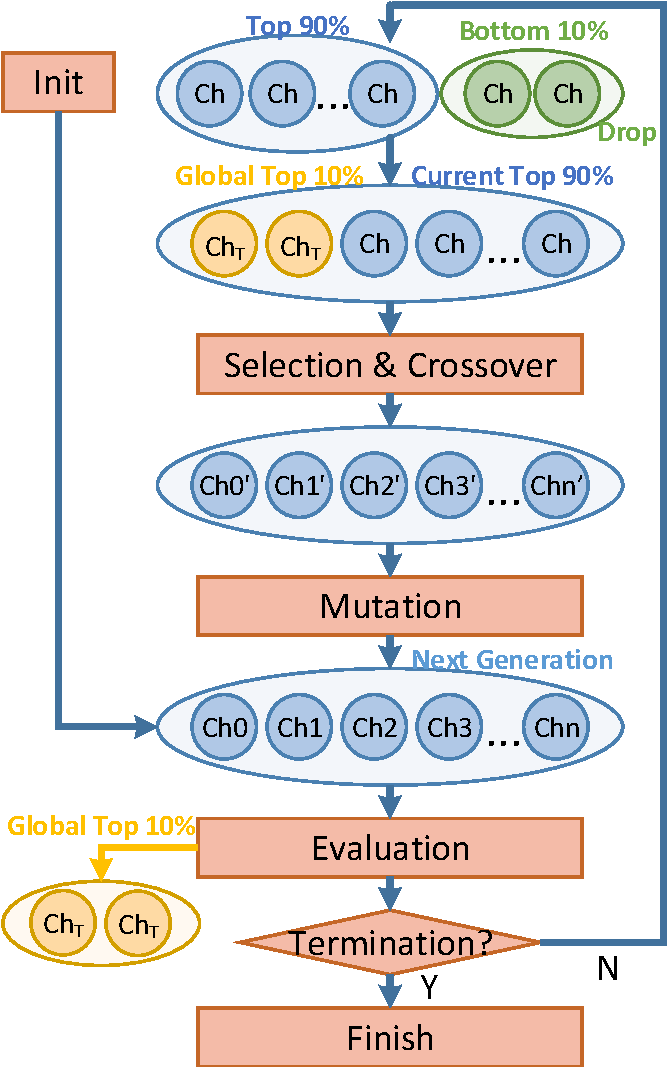
\includegraphics[width=\linewidth]{fig/pGA.pdf}
%	\end{center}
%	\vspace{-5pt}
%	\caption{Algorithm Overview}
%	\label{fig:GA}
%	%\vspace{-4pt}
%\end{wrapfigure}

\begin{figure}[h]
	\centering
	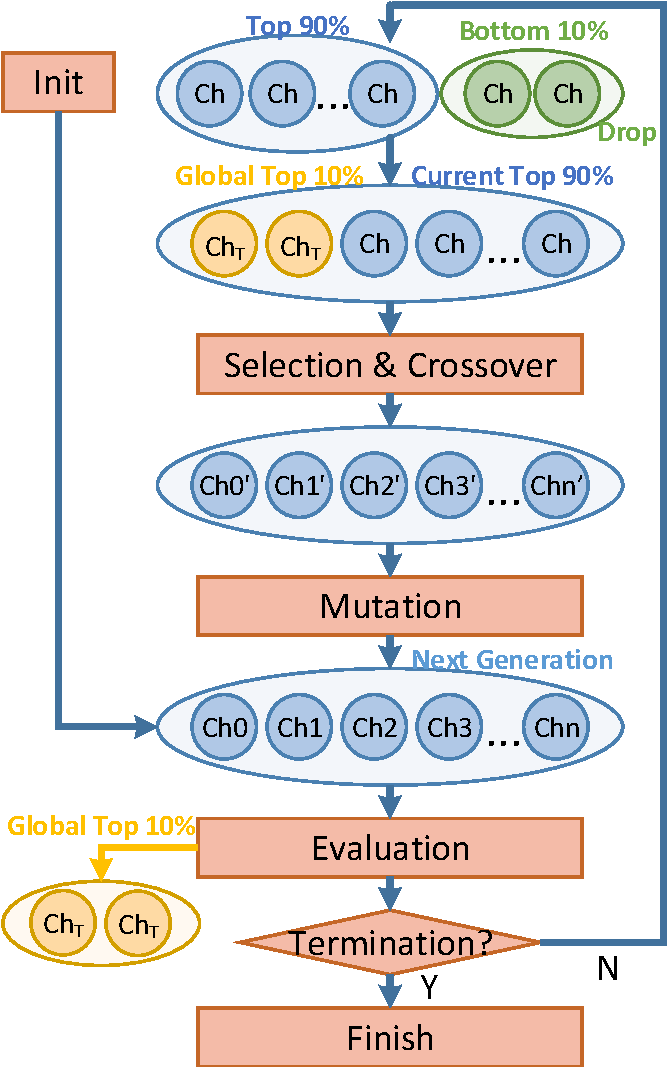
\includegraphics[width=0.5\linewidth]{fig/pGA.pdf}
	\caption{Genetic Algorithm Overview}
	\label{fig:GA}
\end{figure}

\figref{fig:GA} overviews our baseline genetic algorithm. The exploration configuration is captured in a set of \emph{chromosomes}. Each chromosome captures HW/SW mapping of each function type (FT) in the domain as a set of genes. After randomly generating an initial population, the \emph{evaluation} analyzes the fitness of each chromosome using the analytic model. The evaluation tracks global top 10\% chromosomes (across all generations). They replace the bottom 10\% in a generation to start a new population. From this, \emph{Selection \& Crossover} selects pairs of promising chromosomes swaps genes among them. To further increase variation, \emph{Mutation} randomly mutates individual genes. The resulting population is evaluated again and the process repeats until the \emph{Termination} condition is reached. The next paragraphs describe the process in detail. 



\textbf{Chromosome Definition.} An architecture is encoded as a chromosome as a string of integers, see Eq.~\eqref{eq:ch}, representing individual genes in a fixed order. Each gene ($g_A$, $g_B$ .. $g_X$) represents whether a FT ($t_{A}$,$t_{B}$ ... $t_{X}$) is implemented in SW ($g_{I} = 0$) or in HW ($g_{I} > 0$). Adding a repeated ACC with FT existed in HW has less improvement in performance, and wastes the HW budget. To simplify the large domain design space, in this paper, each FT is at most implemented once in HW. Application to platform mapping is implicit: each actor instance of a HW-implemented FT is mapped to its HW accelerator.
As outlined in \secref{sec:Platform} "Target Platform", only HW/SW communication occurs through a common system interconnect through shared memory. Consequently, connectivity, mapping to system communication fabric or memory is not encoded as they can be inferred from the HW allocation. Connectivity within the HW partition is n:n, neither needing encoding.
%
\begin{equation}
%\vspace{-6pt}
\begin{split}
\label{eq:ch}
&Ch = \{g_A, g_B, ..., g_X \}, \left\vert{Ch}\right\vert = \left\vert{T}\right\vert \\
&g_{I} = 0, t_{I} \in SW \\
&g_{I} > 0, t_{I} \in HW \\
\end{split}
\end{equation}


\textbf{Initialization.} To form the starting population, \emph{init} randomly generates chromosomes according to the defined HW budget $N$ (i.e. $\lvert HW \rvert = N$, and $\lvert SW \rvert = \lvert T \rvert - N$). The population size is dependent on the design space, which given our assumptions is mostly impacted by the number of function types $\lvert T \rvert$. Therefore, we scale the population size dependent on domain by: $\lvert P  \rvert = \lfloor 2 * \sqrt{ \lvert T \rvert} \rfloor$.

\textbf{Evaluation / Fitness Function.} Evaluating the fitness of a single chromosome requires \emph{evaluating} each domain application on the platform encoded in the chromosome, as well as \emph{aggregating} the results. Our our analytical model \secref{sec:EvaOp} computes steady state throughput for each app. To obtain a comparable quantification across apps we consider throughput improvement: scaling throughput on the candidate platform over throughput of a pure SW platform.  The \emph{aggregation} across all applications' throughput improvement determines how well the applications are represented in the domain. As we aim for an equal representation, the applications' throughput is averaged to determine the chromosome's fitness. 

To reduce the number of generations needed for a complete exploration, \ga applies an elitist bias \cite{quan2014towards}. Chromosomes are sorted by fitness. The fittest 10\% chromosomes are promoted to a global elite pool maintained across all generations. As the global elite pool is of constant size, the most elite chromosomes displace less elites. To form a new population the bottom 10\% chromosomes are dropped and replaced with the elite pool. This allows the elite genes to breed into the next generation. 

% JH very detailed question: if one generation has a chromosome propagated to the elite pool. Then this elite chromosome will be swapped back in from the elite pool. Does the SAME chromosome then exist twice in the population (once from the top 90\% of the generation and once from the elite pool)?
% JH: yes same chromosome will exist twice -> higher chance to be chosen


\textbf{Selection \& Crossover.}
From this initial pool, a weighted roulette wheel \emph{selects} chromosomes for crossover. Fitter chromosomes (using the prior evaluation results) are more likely to be selected than less fit ones. Thus, the selection prefers fitter parents with the aim to propagate the best genes, but also allows others to foster diversity. For a selected pair of parent chromosomes, the crossover stage randomly selects which genes are inherited from each parent parents (subject to the HW budget). The selection and crossover repeats until a complete new population is formed.
% cross over is for |P| times to generate |P| new chromosomes 
% HW budget exeeded: repeat selection and cross over

\textbf{Mutation.} 
After crossover, the chromosomes are subject to mutation. It randomly selects two genes with opposite state (HW/SW allocation) and inverses their state.  

%The process of crossover and mutation repeats until a population out of only new chromosomes (result of crossover and mutation) is constructed. 
% first all cross over then all mutation 

\textbf{Termination.}
Given the new population the process repeats again with evaluating the fitness of each chromosome. The GA terminates if the best solution (i.e. the fittest chromosome from the elite pool) has not improved in the last 10 generations or the maximum number of generations (100) is reached. 
% actual implementation: OpenVX and synth are with 20 fixed generatiosn
% scaling experiments stops after 10 wihtout improvment
% observed 16 generations for small, 29 for large (100 types)
% max number is theoretical (not actually implemented)


%GS disabled the stuff below as it basically repeats as intro in the next section

%While a random genetic algorithm can perform well for an application DSE, we have found that it still takes too long for domain-DSE as it relies on random mutation without guidance. To improve exploration speed, we introduce a guided local search for the mutation. The next three sections discuss alternative approaches for the guided local search. 

%Heuristic Guided Mutation

\subsection{\ga with Guided Local Search}
\label{sec:GALS}

Purely random mutation requires many generations to converge. To enhance the exploration performance, \ga employs a guided local search inspired by ~\cite{wen2011heuristic}. For each chromosome it searches for the best neighbor to propagate (instead of random mutation). The evaluation methodology for the local search is crucial for the overall exploration performance. \ga uses a hybrid approach between Domain Score (DS) and Analytic Evaluation (AE) model. In order to simplify explanation and to enable details analysis, we introduce two simpler variants first: \gads and \gaana.

%It first finds the best neighbor of a chromosome by exhaustively switching two genes with opposite states (i.e. replacing a function type for HW implementation), and then evaluates the benefit of each swap. With respect to evaluation method, we proposed three variations: (1) \gads, (2) \gaana, and (3) \gah which is the ultimate \ga implementation. 

%Instead of the random mutation implemented in GA-Random,  \emph{\gads} performs a guided local search, see \figref{fig:GADSS}, 

%We consider three variants (sorted by complexity) for guided local search: (1) a guided local search using the proposed Domain Score (\gads), (2) a guided local search using the proposed Analytical Model (\gaana) for evaluation, (3) our complete approach, \ga, which employs a hybrid DS and Analytical Model, combining their benefits.  


\subsubsection{\gads}
\label{sec:GALS-DSS}

\figref{fig:GADSS} illustrates the guided local search used instead of random mutation of \garand. \gads finds the best neighbor of a chromosome $Ch_{cur}$ by exhaustively switching two genes with opposite states, and then evaluates the benefit of each swap using \newtext{the Domain Score (DS),} see~\secref{sec:ds}.

\newtext{After finding the best neighbor}, \gads keeps the best neighbor $Ch_{BN}$ (i.e. mutation with the most benefit) over the starting chromosome $Ch_{cur}$. If the best neighbor $Ch_{BN}$ improves DS, it then becomes $Ch_{cur}$ the starting point for the next search and the process repeats. 

The search terminates if no improvement is found. The last $Ch_{BN}$ becomes one chromosome in next generation. If the first search iteration does not find any improvement, the search terminates immediately and instead of $Ch_{cur}$ a new random chromosome $Ch_{R}$ is inserted. This increases the random variation and thus the chance to escape a local optimum in the following generation(s). The local search process repeats for each chromosome $Ch0' .. Chn'$. 



\begin{figure}[h]
	\centering
	%\vspace{-10pt}
	\subfloat[GA-LS(DS),GA-LS(AE) ]{
		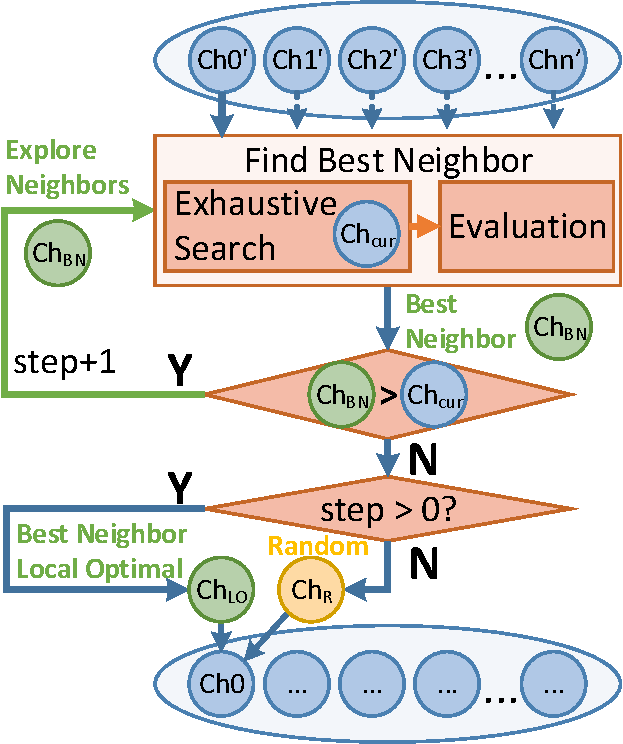
\includegraphics[width=.45\linewidth]{fig/pGADSS.pdf}
		\label{fig:GADSS}}
	\hfill
	\subfloat[GA-LS(Hybrid)]{
		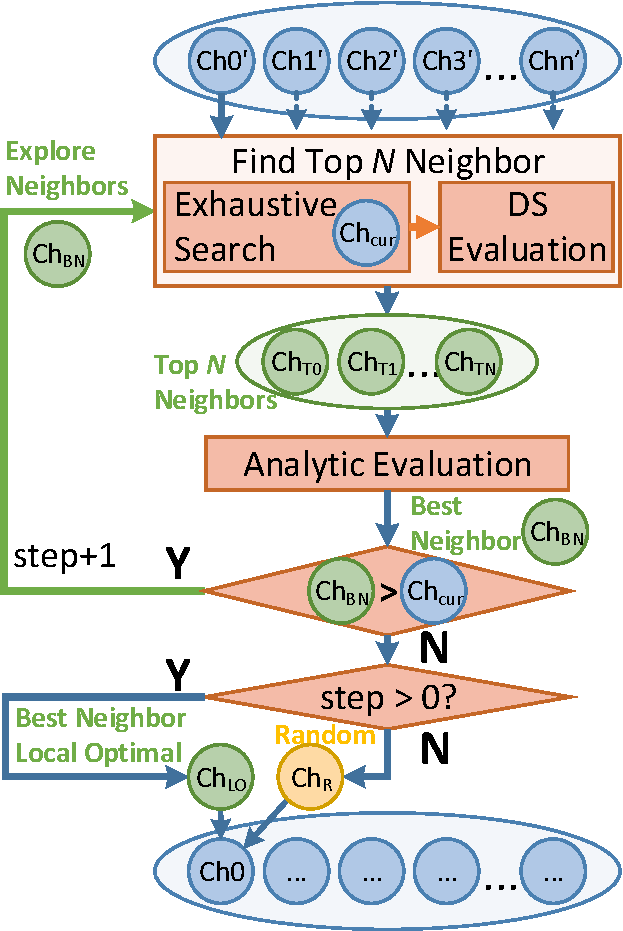
\includegraphics[width=.45\linewidth]{fig/pGADSSA.pdf}
		\label{fig:GAHybrid}}
	%\vspace{-5pt}
	\caption{Guided Local Search}
	%\vspace{-8pt}
\end{figure}

%Local search an iterative algorithm that starts with one solution, then attempts to find the best neighbor solution by exhaustive evaluate all neighbors. If the best neighbor produces a better solution compared with the original one, the best neighbor is made to the new solution, repeating until no further improvements can be found.
%In our GA algorithm, the solution is the chromosome, which defining the domain SW / HW partitioning. The neighbors of the chromosome, are (1) migrating one function type from SW(HW) to HW(SW), and (2) swap a pair of function types between SW and HW.

%Apply local search for each chromosome in generation. Using DSS to evaluate all neighbors of this chromosome, and find the best neighbors as the next step, if it has improvement. Search until no longer improvement. At the end, the mutation finds top 1 candidate (local optimal architecture) for each chromosome to form the new generation.

%If the original chromosome has been evaluated before or it is already the local optimal solution, which local search step is equal to 0, and cannot find a better neighbor in the first step of local search.
%The GA random generated a new chromosome for next generation, to help our GA to explore the large design space with more diversity.

%TODO GS Idea if the best chromosome was created just by cross over. Then, we will discard it with the approach above and replace it with a random chromosome. In effect: the absolute best solution can only be found through mutation in our setting. Improvement: after selection & chross over to a ranking by DS. Top X% of ranked chromosomes are not displaced by random, if no further improvement is found. 





\subsubsection{\gaana}

The just introduced \emph{\gads} favors speed over accuracy using the DS for evaluation in the neighborhood search. While DS is the fastest evaluation, it has limited accuracy (see \secref{sec:eva:sum}). In order to quantify the impact, we introduce the more accurate \emph{\gaana}. It realizes the same search as \emph{\gads}, however, uses the analytical model for evaluation. As the analytical model computes the performance of a single application, each application in the domain has to be evaluated and the results aggregated to determine the chromosome's fitness. This is identical to the \emph{evaluation} in \emph{\garand}. In result, the \gaana performs a very accurate local search, at the cost of exploration speed. 
\subsubsection{\gah}

In order to combine the benefits of \gads speed  and \gaana accuracy in the local search, we introduce \gah combining both approaches.

The exhaustive search over the local neighbors significantly impacts overall exploration performance. It evaluates many alternatives ($ \sum_{1 .. \lvert P \rvert} Steps_{i} * N * (\lvert T \rvert - N)$). Even considering only 1 step for each chromosome ($\lvert T \rvert$ = 50, $N$=10), already 5600 alternatives are evaluated. Hence, the fastest evaluation possible is paramount. To achieve this, \gah employs a two step approach: it first uses the faster (but less accurate) DS to identify a group of best neighbor candidates, and then re-evaluates those using the more accurate (but slower) Analytical Model to find the best neighbor. See \figref{fig:GAHybrid}. 

\gah first uses the faster evaluation \emph{DS} to find through exhaustive search the $N$ best neighbors ($Ch_{BN0}$ .. $Ch_{BNN}$) for a given chromosome $Ch_{cur}$. It then uses the analytic evaluation to select the best neighbor $Ch_{BN}$ from these candidates. The termination and random chromosome insertion are identical to \gads.

Dimensioning the group size is a local speed/accuracy trade-off. For our experiments, we opt to compare the top 5 neighbor candidates. We postulate that DS is sufficiently accurate to delineate from 400 down to 5 candidates ($\lvert T \rvert$ = 50, $N$=10). In addition, finding the absolute best in each step is not necessary as the search is iterative, improving in the next local step (or generation).


%\begin{figure}[htbp]
%	\centering
%	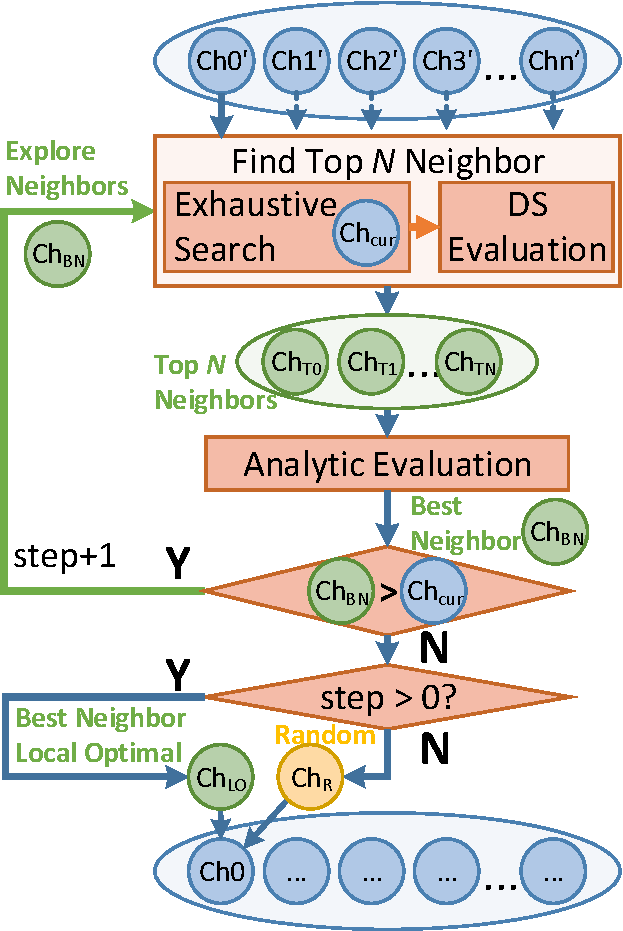
\includegraphics[width=0.48\linewidth]{fig/pGADSSA.pdf}
%	\caption{Guided Local Search (Hybrid)}
%	\label{fig:GAHybrid}
%\end{figure}



\subsection{\ga Versions Comparison}

\begin{table}[h]
	\caption{Different \ga \newtext{Comparison}}
	\label{tab:GIDE}
	\centering
	\begin{tabular}{p{0.29\linewidth}|p{0.12\linewidth}|p{0.1\linewidth}|p{0.13\linewidth}|p{0.12\linewidth}}
		\toprule
		   & GIDE-RANDOM & GIDE-DS  & GIDE-ANALYTIC & GIDE-HYBRID \\
		\hline
		\midrule
		\textbf{Local Search} & - & Y & Y & Y \\
		\hline
		\textbf{Domain Score guided} & - & Y & - & Y \\
		\hline
		\textbf{Analytic Eval guided} & - & - & Y & Y \\
		\bottomrule
	\end{tabular}
\end{table}

\tabref{tab:GIDE} \newtext{summaries the different versions of GIDE described in previous sections.} \garand \newtext{is normal genetic algorithm  without guided local search in mutation.} \gads and \gaana \newtext{are genetic algorithms with one level guided local search.} \gads \newtext{uses the Domain Score (DS) to guide local search, which has high speed but low accuracy of estimation.} While \gaana \newtext{has slow but high accurate guided local search, using Analytic Evaluation (AE).} \gah \newtext{has two-level guided, combining DS and AE, which balance the speed and accuracy.}  



 %The heuristics methods are comprised of an algorithm to explore design space and a fast evaluation/estimation to judge the performance/benefit of each iteration/selection.

%Given the very large design space, methods for efficiently traversing the design space, such as genetic algorithms \cite{abdeen2014multi}, simulated annealing \cite{liang2013hardware}, tabu search \cite{wu2013efficient}, and greedy algorithms \cite{tang2015hardware}, are important. 

% need to describe the problem.
% see also end of 3.2 




%%\vspace{-4pt}
\section{Experimental Results}
\label{sec:results}


This section evaluates the benefits and costs of DSS and \ga from different angles. After defining the experimental setup, it first looks at a global comparison. It then gives insights to the individual variants, followed by analyzing the scalability with increasing domain size. Finally, it quantifies how well unknown applications can be supported.


\subsection{Experimental Setup}

Evaluating a Doman DSE requires comparing over large set of applications, approaches and platforms. We use throughput improvement as a primary performance metric for a domain platform. It scales the applications throughput executing on the candidate platform over a complete SW implementation, quantifying speedup. We evaluate \newtext{DSS and} each version of \ga domain platforms, 
and compare against a full exhaustive search (where possible), \newtext{which evaluate all domain applications on the domain platform, see} \figref{fig:DomainP}.


To understand the performance difference between domain-specific platform and application-specific platforms we build on the definitions in~\cite{zhang100ds}. Each application has an own OPTimal application-specific architecture (OPT) that maximizes the application throughput, see ~\figref{fig:OOP}. 
The OPT is obtained through (time consuming) exhaustive search. 
Executing each application in a domain on its own OPT yields the upper bound: \textbf{Own OPT Platform (OOP)} -- indicating the acceleration potential of a domain given a HW budget. In order to understand the penalty of application-specialization, we consider \textbf{Foreign OPT Platform (FOP)}, see \figref{fig:FOP}. Here, each application is evaluated multiple times, once on each platform in the pool of OPT (all but one being foreign to the application).



\begin{figure}[h]
	%\vspace{-5pt}
	\centering
		\subfloat[Domain Plat]{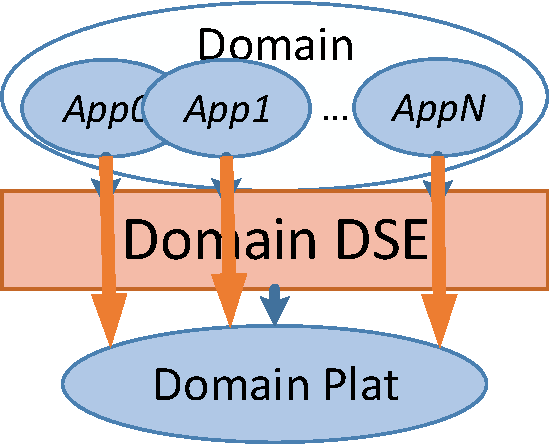
\includegraphics[width=.28\linewidth]{fig/pDomainP.pdf}\label{fig:DomainP}}
		\hfill
		\subfloat[OOP]{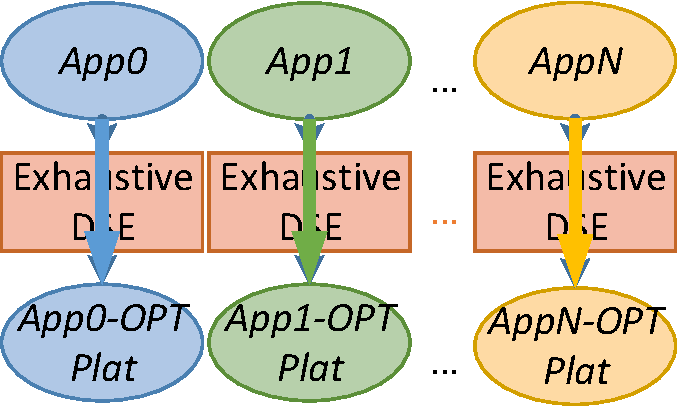
\includegraphics[width=.32\linewidth]{fig/pOOP.pdf}\label{fig:OOP}}
		\hfill
		\subfloat[FOP]{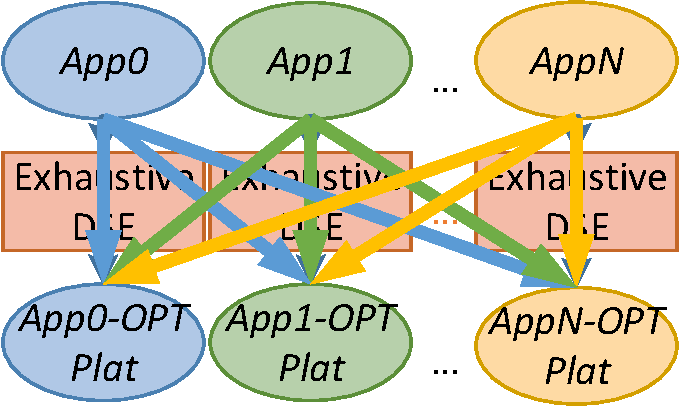
\includegraphics[width=.32\linewidth]{fig/pFOP.pdf}\label{fig:FOP}}
	%\vspace{-5pt}
	\caption{Experiments Settings}
	%\vspace{-4pt}
\end{figure}



We evaluate two domain types. The \textbf{OpenVX} domain (computer vision) has 35 function types and contains 40 applications from Intel \cite{Intel} and AMD \cite{AMD}, abstracted into data flow models. The \textbf{synthetic} domain is generated with 50 function types, containing 100 applications with a balance between processing and communication. 
%Performance is evaluated on automatically generated virtual platforms (SCE\cite{domer2008system}) capturing the abstract data flow model (SDF3\cite{stuijk2006sdf}) and architecture resources. 
The target platform contains a processor with N ACCs. Communication occurs on a 3R3W layer bus. The processing speedup on ACCs should be variable for different FTs, which could be implemented in different models, e.g. roofline model. For simplification, this paper just assumes ACC processing is 20x faster than SW. ACCs can communicate directly with each other~\cite{teimouri2016improving}.

\subsection{Domain Throughput Comparison}
\label{sec:resTh}

To gain a first global view, \figref{fig:th} plots the throughput improvement of the two domains over increasing HW budget.

%Graph is Average Throughput Improvement
\begin{figure}[htb]
	%\vspace{-10pt}
	\centering
		\subfloat[OpenVX Domain]{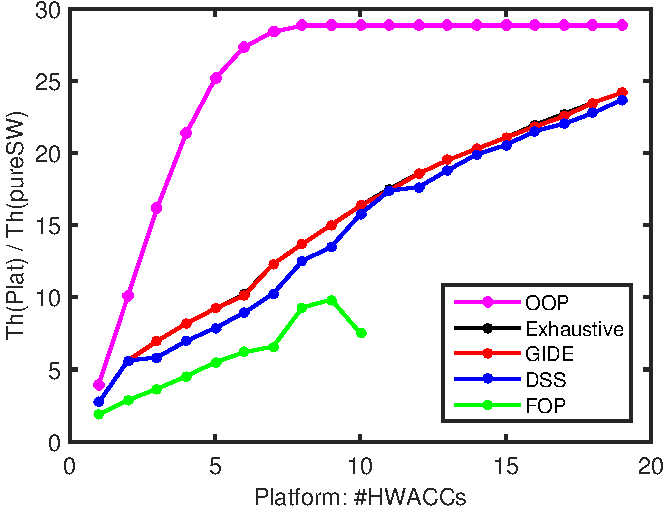
\includegraphics[width=.48\linewidth]{fig/prThOpenVX.pdf}\label{fig:thOpenVX}}
		\hfill
		\subfloat[Synthetic Domain]{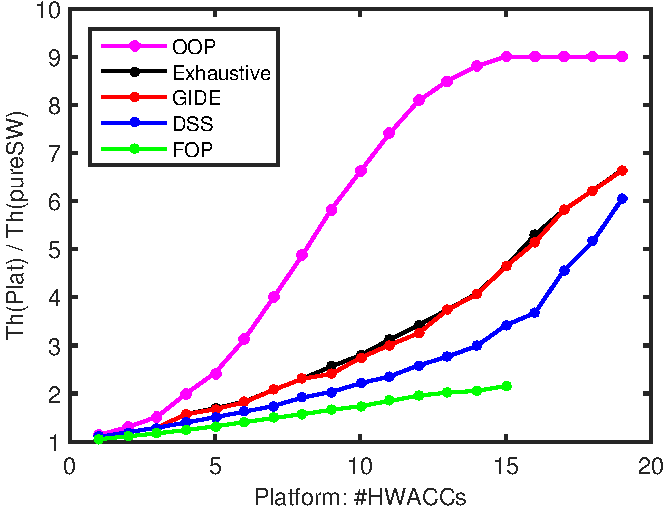
\includegraphics[width=.48\linewidth]{fig/prThSyn.pdf}\label{fig:thSyn}}
	%\vspace{-5pt}
	\caption{Average throughput improvement}
	\label{fig:th}
	%\vspace{-4pt}
\end{figure}

\textbf{OOP} yields highest (but unrealistic) throughput, see \figref{fig:thOpenVX}, assuming that each application were to execute on its own OPT. This indicates the acceleration potential. It saturates with budget $N$=10, when each application has enough accelerators. However, considering a single platform for all applications, \textbf{Exhaustive} indicates the optimum. It linearly increases with $N$ closing the gap to OOP, indicating that the additional area is well invested. \textbf{\ga} (actually \gah) almost achieves domain optimal, tracking Exhaustive. The greedy \textbf{DSS} is measurably below optimum but the gap narrows with budget. Exploring at application scope incurs dramatic penalties as indicated with \textbf{FOP} on the bottom.
FOP plateaus with 10 ACCs as already all possible ACCs have been selected for each application and it cannot outside this application to accelerate.
Comparing against FOP, \ga and DSS have 74.85\% and 58.02\% higher throughput ($N$\textless=10).

The synthetic domain, \figref{fig:thSyn}, exhibits similar trends. OOP and FOP saturate later $N$=15 due to the larger domain (more function types). Given larger domain, the gap between DSS and GA is increased. As the synthetic domain has a larger design space, the DSE performance has more impact on the results. Here, \ga and DSS have a 48.09\% and 23.60\% higher throughput ($N$\textless=15).

In order to better delineate DSE performance, we define the metric \textbf{average throughput achievement}. It scales the throughput improvement of a DSE generated platform over the throughput improvement of the domain optimal platform (i.e. Exhaustive) of the same budget. An throughput achievement of 1 thus indicates the optimum. \figref{res:pa} graphs the achievements.

%Graph is Performance Achievement
\begin{figure}[htbp]
	%\vspace{-10pt}
	\centering
		\subfloat[OpenVX Domain]{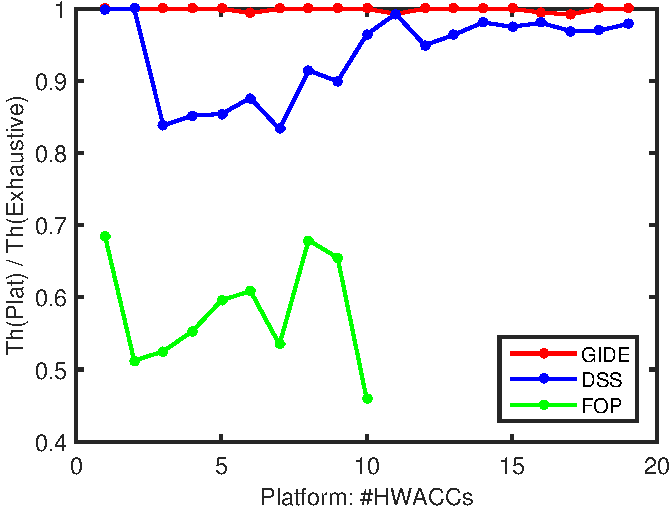
\includegraphics[width=.48\linewidth]{fig/prPAOpenVX.pdf}\label{fig:paOpenVX}}
		\hfill
		\subfloat[Synthetic Domain]{\includegraphics[width=.48\linewidth]{fig/prPASyn.pdf}\label{fig:paSyn}}
	%\vspace{-8pt}
	\caption{Average Throughput Achievement}
	\label{res:pa}
	%\vspace{-4pt}
\end{figure}

In \figref{fig:paOpenVX}, \ga achieves close to the optimum, with 99.87\% on average across all budgets for the OpenVX domain. DSS achieves less with 93.65\% and is not as stable. FOP has a large gap with only 58.07\%.

Considering the larger synthetic domain, \figref{fig:paSyn} shows even more differentiation. GA, DSS, FOP achieve 98.84\%, 83.45\% and 69.81\%, respectively. The gap between DSS and GA is more pronounced and largest gap shifts from $N$=7 in OpenVX to $N$=16 in synthetic domain. Beyond that point, DSE performance is not as critical as with a higher HW budget the margins between the ACCs selection become smaller, thus selecting a sub-optimal ACC has a lower penalty.



\subsection{\ga Variant Analysis}
\label{sec:resMutation}

In order to understand the DSE contributions of individual \ga aspects, we analyze the variants with respect to throughput achievement and exploration time of the synthetic domain, see \figref{fig:dse:tr}.

%Graph show the GA+LS(Hybrid) is the best.
\begin{figure}[h]
	\centering
	%\vspace{-10pt}
	\subfloat[Throughput Achievement]{\includegraphics[width=.48\linewidth]{fig/prPAGASyn.pdf}\label{fig:paGASyn}}
	\hfill
	\subfloat[Exploration Time]{\includegraphics[width=.48\linewidth]{fig/prTimeGASyn.pdf}\label{fig:timeGASyn}}
	%\vspace{-5pt}
	\caption{Comparing \ga Variants (Synthetic)}
	\label{fig:dse:tr}
	%\vspace{-10pt}
\end{figure}




\gah and \gaana exhibit very similar achievements, see Fig.~\ref{fig:paGASyn}. They are close to optimal which is 99.41\% and 98.84\%, respectively, increasing the confidence in selecting the hybrid approach. Conversely, \gads is hampered with the DS accuracy in the guided local, only achieving 89.20\%. The inaccuracy of DS can lead to getting the local search being stuck at an invalid local optimum. \garand has the lowest achievement with 79.90\% on average over budget.

Looking at exploration time, \figref{fig:timeGASyn}, \garand is the fastest with 2 seconds. \gads, \gah and \gaana are around 5x, 100x, 10000x slower than random mutation. 
%
Comparing both achievement and exploration time sets out \gah as the best choice being 100x faster than \gaana while still achieving close to optimum results. Its two step of initial pruning with DS followed by more detailed analytic evaluation clearly sets it apart.  


\begingroup
\setlength{\columnsep}{8pt}%

\begin{wrapfigure}{l}{0.5\linewidth}
	%\vspace{-6pt}
	\begin{center}
		\includegraphics[width=\linewidth]{fig/prPAGenSyn.pdf}
	\end{center}
	%\vspace{-8pt}
	\caption{Improvement per Generation}
	\label{fig:paGenSyn}
	%\vspace{-4pt}
\end{wrapfigure}


To gain more insight with exploration generations, \figref{fig:paGenSyn} explores the achievement for a constant budget of $N$=19 in the synthetic domain. \gaana is the fastest to reach the best solution in only 5 generations. \gah is only 2 generations behind. \gads although rapidly reaching 90\% in a few generations, it cannot improve much over the remaining generations as it is stuck in an inaccurate local maximum. \garand needs many more generations, but steadily improves over them. 

\endgroup
%\begin{figure}[h]
%	\centering
%		\subfloat[OpenVX Domain]{\includegraphics[width=.5\linewidth]{fig/prPAGenOpenVX.pdf}\label{fig:paGenOpenVX}}
%		\hfill
%		\subfloat[Synthetic Domain]{\includegraphics[width=.5\linewidth]{fig/prPAGenSyn.pdf}\label{fig:paGenSyn}}
%	\caption{Improvement per Generation}
%\end{figure}

%\begin{figure}[h]
%	\includegraphics[width=.75\linewidth]{fig/prStepLimit.pdf}
%	\caption{OpenVX: GA limit number steps of local search}
%	\label{fig:stepLimit}
%\end{figure}



Our measurements demonstrate that the guided local search is highly efficient. To gain even further insight we measure
the average number of search steps and the effect of artificially limiting the search depth when exploring the OpenVX domain.
%Graph to show the step number of local search is acceptable. (Graph is need to re-draw)
\begin{figure}[h]
	\centering
		\subfloat[Average \# of Steps]{\includegraphics[width=.48\linewidth]{fig/prStepAve.pdf}\label{fig:stepAve}}
		\hfill
		\subfloat[Limit Steps of Local Search]{\includegraphics[width=.48\linewidth]{fig/prStepLimit.pdf}\label{fig:stepLimit}}
	\caption{Local Search Steps}
	\label{fig:step}
\end{figure}


%\begingroup
%\setlength{\columnsep}{8pt}%

%\begin{wrapfigure}{l}{0.5\linewidth}
	%\vspace{-6pt}
%	\begin{center}
%		\includegraphics[width=\linewidth]{fig/prStepLimit.pdf}
%	\end{center}
	%\vspace{-8pt}
%	\caption{Limit Steps of Local Search}
%	\label{fig:stepLimit}
	%\vspace{-4pt}
%\end{wrapfigure}

\newtext{In} \figref{fig:stepAve}, \gaana, \gah and \gads have all a very low number of average steps across generations with, 2.91, 2.37, and 2.41 respectively. Even its maximum is low with 10 (\gaana), and 8 (for both \gah and \gads). The low number of steps can be explained with the exhaustive search of the neighborhood. Sparser sampling approaches, conversely, would need more steps. Limiting the maximum number of search steps only minimally impacts search performance as shown in \figref{fig:stepLimit} for the OpenVX domain. Although limiting to 3 steps, \gah still finds the optimum in 4 steps in this example. Further limiting the number of steps translates into requiring more generations (+3 with 2 steps, +4 with 1 step) nonetheless the same solutions are still reached. Due to the speed of DS evaluation, we do not limit the number of steps. 

%\endgroup

%GA summary - GS CUT
% GA with different mutations Trade-off between throughput achievement and exploration time.
%Summarizing the detailed results confirms our selection of \gah as the most suitable approach providing both s
%Random and DSS have the fast exploration, but the performance is bad.
%The Analytical and Hybrid has the almost highest performance.
%Hybrid is 100x faster than analytical evaluation.
%GA-Hybrid is the best choice for domain DSE for most cases.
%However, if want to get the highest performance design, and do not care about the exploring time, the GA-analytical could be considered.
\subsection{Scalability with Increasing Domain Size}
\label{sec:res:size}

%Domain Analyzer Time
\newtext{The exploration time to identify a domain-specific platform using our approach consists of two parts: domain analysis and design exploration. The initial domain analysis is fast: analyzing the synthetic domain with 100 apps (with up to 12 nodes each) on Intel i5-3450 with 3.10GHz takes 22.1s. Since the initial domain analysis only executes only once, this section mainly focuses on the scalability of domain exploration.} 

%Graph to show the scalability of our graph
Exploration time is correlated to the size of the domain, more specifically: the number of function types. \figref{fig:scale} analyzes the exploration time as well as the achievement over number of function types to measure scalability. 

\begin{figure}[h]
	%\vspace{-5pt}
	\centering
		%\subfloat[FT=50, diff HW budget]{\includegraphics[width=.5\linewidth]{fig/prTimeHW.pdf}\label{fig:timeHW}}
		\subfloat[Exploration Time]{\includegraphics[width=.5\linewidth]{fig/prTimeSpace.pdf}\label{fig:timeSpace}}
		\hfill
		\subfloat[Relative Throughput]{\includegraphics[width=.5\linewidth]{fig/prPASpace.pdf}\label{fig:paSpace}}
	%\vspace{-4pt}
	\caption{Scalability with Domain Size}
	\label{fig:scale}
	%\vspace{-8pt}
\end{figure}

\figref{fig:timeSpace} shows that with increasing design space, DSS and \ga scale well only slowdown linearly. The orders of magnitude comparisons hold with these approaches across size. Conversely, the Exhaustive search exponentially increases exploration time (estimation only). The benefits are most predominant with the largest domain (FT=100). Here, \gah is $4.6*10^{13}$ times faster than exhaustive.

Fig.~\ref{fig:paSpace} illustrates the stability of results over increasing domain size. However, obtaining the domain optimal platform is infeasible due to exorbitant long exploration time ($3*10^8$ years, FT=100). As an approximation, \figref{fig:paSpace} shows relative throughput compared to \gaana. Even over large domains \gah scales very well and its results remain close to \gaana with 97.51\% on average. Conversely, the limitations of DSS become more pronounced as domain size increases (63.16\%).

%Performance over increasing domain size. The first graph should be changed to performance versus time.
%\begin{figure}[H]
%	\centering
%		\subfloat[Relative Throughput]{\includegraphics[width=.5\linewidth]{fig/prPASpace.pdf}\label{fig:paSpace}}
%		\hfill
%		\subfloat[Performance vs Time]{\includegraphics[width=.5\linewidth]{fig/prPATimeSpace.pdf}\label{fig:paTimeSpace}}
%	\caption{Synthetic Domain: HW=19, with diff design space}
%\end{figure}

%Fig.~\ref{fig:paTimeSpace} trade-off. GA Hybrid could achieve high performance, with less exploring time compared with GA-analytical. Although the DSS is much faster than other two algorithm, it could get the good domain platform.
\subsection{Effects of Unknown Applications}
\label{sec:res:unknown}

The quality of a domain platform is also expressed in how well it supports applications unknown at design time. We explore the effect for the OpenVX domain. For this, the DSE is performed with N-1 domain applications. Throughput measurements, conversely, are performed using \newtext{the unknown application.} The process is repeated N times and results averaged. \figref{fig:unknown} reports the results.

\begin{figure}[h]
	%\vspace{-5pt}
	\centering
		\subfloat[Average Throughput Improvement]{\includegraphics[width=.5\linewidth]{fig/prUnknowTh.pdf}\label{fig:unknownTh}}
		\hfill
		\subfloat[\newtext{Cumulative Performance Loss} (HW=8)]{\includegraphics[width=.47\linewidth]{fig/prUnknowCD.pdf}\label{fig:unknownCD}}
	%\vspace{-8pt}
	\caption{N-1 Training, 1 Evaluation Rotating (OpenVX)}
	\label{fig:unknown}
	%\vspace{-6pt}
\end{figure}

As \figref{fig:unknownTh} shows that even the exhaustive search exhibits a significant loss over \textbf{DomainOPT} which is the oracle solution knowing all applications at design time. Comparing DSE approaches is inconsistent, as each is at least once the best due to averaging.  

\figref{fig:unknownCD} reveals much more insight showing the cumulative distribution of application throughput achievement (over DomainOPT) for a budget of 8 (where DSS had highest average improvement). 
Exhaustive and \ga show a much better distribution than DSS. In Exhaustive and \ga more than 80\% applications could achieve highest throughput. 
The reason of higher DSS average, is that DSS fully accelerate some applications which have a very high individual throughput improvement.  However, for a large size of low throughput improvement, the DSS can not accelerate it. 


%\begin{figure}[H]
%	\centering
%	\includegraphics[width=.7\linewidth]{fig/resPerfLoss.pdf}
%	\caption{OpenVX: Throughput Loss Cumulative Distribution}
%	\label{fig:resOpenVXLoss}
%\end{figure}

%\vspace{-5pt}
\subsection{Generalization}
\label{sec:generalization}
%\vspace{-3pt}

Our analysis is best summarized as the DSE trade-off between exploration time and achieved performance. \figref{fig:paTime} quantifies the trade-off for OpenVX and synthetic domain. 


\begin{figure}[H]
	%\vspace{-5pt}
	\centering
		\subfloat[OpenVX Domain]{\includegraphics[width=.5\linewidth]{fig/prPATimeOpenVX.pdf}\label{fig:paTimeOpenVX}}
		\hfill
		\subfloat[Synthetic Domain]{\includegraphics[width=.5\linewidth]{fig/prPATimeHWSyn.pdf}\label{fig:paTimeHWSyn}}
		%\vspace{-6pt}
	\caption{Design Exploration trade-off}
	\label{fig:paTime}
		%\vspace{-6pt}
\end{figure}

As domain size increases the trade off becomes more pronounced, i.e. it is more visible for the synthetic domain \figref{fig:paTimeHWSyn}. 
DSS achieves the fastest results but with low accuracy. \garand is similar in accuracy but much slower. DSS outperforms \garand as it uses domain features to guide the exploration. \gads produces designs with limited performance as it is limited by DS accuracy. Both \gah and \gaana approach optimal performance, while \gah is 100x faster. This makes \gah the preferred approach for DS-DSE.


%\section{Conclusion}

\label{sec:conclusion}
\newtext{This paper introduced a Domain-specific Design Space Exploration (DS-DSE) methodology to broaden the scope of existing DSE from individual apps in isolation to a whole domain. This paper lays the foundations by defining a domain and quantifiable features (metrics) that can guide exploration. The features take both behavioral (processing) and structural (communication) aspects into account, as well as consider the distribution over the domain.} 

\newtext{Based on these definitions, the paper has introduced the Dynamic Score Selection (DSS) and GenetIc Domain Exploration (GIDE) algorithms for domain exploration. These algorithms maximize domain throughput creates a domain-specific architecture that has more flexibility to execute domain applications. DSS uses Domain Score (DS) to estimate platform performance in the domain level.} \ga employs a guided local search with hybrid analytical and DS evaluation models to enhance the domain exploration efficiency. \newtext{Our experimental results (Synthetic and OpenVX domains) demonstrate that} DSS achieves 23.60\%-58.02\%, and \ga achieves 48.09\%-74.85\% performance improvement compared to application-specific FOP platform. \ga almost achieves domain optimal throughput (97.6\% to 99.8\%), with around $1*10^{13}$ faster compared with exhaustive search.

%This paper introduced a novel algorithm, GenetIc Domain Exploration (GIDE), for rapid Domain-specific Design Space Exploration (DS-DSE). The significance of \ga is broadening the scope of the genetic algorithm from a single application to a domain of applications. It employs a guided local search with hybrid analytical and domain score evaluation models to enhance the domain exploration efficiency. Our experimental results show that \ga almost achieves domain optimal throughput (97.6\% to 99.8\%), with around $1*10^{13}$ faster compared with exhaustive search. \ga also achieves 10.65\% to 19.81\% and 48.09\% to 74.85\% higher domain throughput  compared against domain-specific DSS \cite{zhang100ds} and application-specific FOP platforms.

% The very first letter is a 2 line initial drop letter followed
% by the rest of the first word in caps.
% 
% form to use if the first word consists of a single letter:
% \IEEEPARstart{A}{demo} file is ....
% 
% form to use if you need the single drop letter followed by
% normal text (unknown if ever used by the IEEE):
% \IEEEPARstart{A}{}demo file is ....
% 
% Some journals put the first two words in caps:
% \IEEEPARstart{T}{his demo} file is ....
% 
% Here we have the typical use of a "T" for an initial drop letter
% and "HIS" in caps to complete the first word.

% You must have at least 2 lines in the paragraph with the drop letter
% (should never be an issue)



% needed in second column of first page if using \IEEEpubid
%\IEEEpubidadjcol


% An example of a floating figure using the graphicx package.
% Note that \label must occur AFTER (or within) \caption.
% For figures, \caption should occur after the \includegraphics.
% Note that IEEEtran v1.7 and later has special internal code that
% is designed to preserve the operation of \label within \caption
% even when the captionsoff option is in effect. However, because
% of issues like this, it may be the safest practice to put all your
% \label just after \caption rather than within \caption{}.
%
% Reminder: the "draftcls" or "draftclsnofoot", not "draft", class
% option should be used if it is desired that the figures are to be
% displayed while in draft mode.
%
%\begin{figure}[!t]
%\centering
%\includegraphics[width=2.5in]{myfigure}
% where an .eps filename suffix will be assumed under latex, 
% and a .pdf suffix will be assumed for pdflatex; or what has been declared
% via \DeclareGraphicsExtensions.
%\caption{Simulation results for the network.}
%\label{fig_sim}
%\end{figure}

% Note that the IEEE typically puts floats only at the top, even when this
% results in a large percentage of a column being occupied by floats.


% An example of a double column floating figure using two subfigures.
% (The subfig.sty package must be loaded for this to work.)
% The subfigure \label commands are set within each subfloat command,
% and the \label for the overall figure must come after \caption.
% \hfil is used as a separator to get equal spacing.
% Watch out that the combined width of all the subfigures on a 
% line do not exceed the text width or a line break will occur.
%
%\begin{figure*}[!t]
%\centering
%\subfloat[Case I]{\includegraphics[width=2.5in]{box}%
%\label{fig_first_case}}
%\hfil
%\subfloat[Case II]{\includegraphics[width=2.5in]{box}%
%\label{fig_second_case}}
%\caption{Simulation results for the network.}
%\label{fig_sim}
%\end{figure*}
%
% Note that often IEEE papers with subfigures do not employ subfigure
% captions (using the optional argument to \subfloat[]), but instead will
% reference/describe all of them (a), (b), etc., within the main caption.
% Be aware that for subfig.sty to generate the (a), (b), etc., subfigure
% labels, the optional argument to \subfloat must be present. If a
% subcaption is not desired, just leave its contents blank,
% e.g., \subfloat[].


% An example of a floating table. Note that, for IEEE style tables, the
% \caption command should come BEFORE the table and, given that table
% captions serve much like titles, are usually capitalized except for words
% such as a, an, and, as, at, but, by, for, in, nor, of, on, or, the, to
% and up, which are usually not capitalized unless they are the first or
% last word of the caption. Table text will default to \footnotesize as
% the IEEE normally uses this smaller font for tables.
% The \label must come after \caption as always.
%
%\begin{table}[!t]
%% increase table row spacing, adjust to taste
%\renewcommand{\arraystretch}{1.3}
% if using array.sty, it might be a good idea to tweak the value of
% \extrarowheight as needed to properly center the text within the cells
%\caption{An Example of a Table}
%\label{table_example}
%\centering
%% Some packages, such as MDW tools, offer better commands for making tables
%% than the plain LaTeX2e tabular which is used here.
%\begin{tabular}{|c||c|}
%\hline
%One & Two\\
%\hline
%Three & Four\\
%\hline
%\end{tabular}
%\end{table}


% Note that the IEEE does not put floats in the very first column
% - or typically anywhere on the first page for that matter. Also,
% in-text middle ("here") positioning is typically not used, but it
% is allowed and encouraged for Computer Society conferences (but
% not Computer Society journals). Most IEEE journals/conferences use
% top floats exclusively. 
% Note that, LaTeX2e, unlike IEEE journals/conferences, places
% footnotes above bottom floats. This can be corrected via the
% \fnbelowfloat command of the stfloats package.





% if have a single appendix:
%\appendix[Proof of the Zonklar Equations]
% or
%\appendix  % for no appendix heading
% do not use \section anymore after \appendix, only \section*
% is possibly needed

% use appendices with more than one appendix
% then use \section to start each appendix
% you must declare a \section before using any
% \subsection or using \label (\appendices by itself
% starts a section numbered zero.)
%


%\appendices
%\section{Proof of the First Zonklar Equation}
%Appendix one text goes here.

% you can choose not to have a title for an appendix
% if you want by leaving the argument blank
%\section{}
%Appendix two text goes here.


% use section* for acknowledgment
%\section*{Acknowledgment}


%The authors would like to thank...


% Can use something like this to put references on a page
% by themselves when using endfloat and the captionsoff option.
\ifCLASSOPTIONcaptionsoff
  \newpage
\fi



% trigger a \newpage just before the given reference
% number - used to balance the columns on the last page
% adjust value as needed - may need to be readjusted if
% the document is modified later
%\IEEEtriggeratref{8}
% The "triggered" command can be changed if desired:
%\IEEEtriggercmd{\enlargethispage{-5in}}

% references section

% can use a bibliography generated by BibTeX as a .bbl file
% BibTeX documentation can be easily obtained at:
% http://mirror.ctan.org/biblio/bibtex/contrib/doc/
% The IEEEtran BibTeX style support page is at:
% http://www.michaelshell.org/tex/ieeetran/bibtex/
%\bibliographystyle{IEEEtran}
% argument is your BibTeX string definitions and bibliography database(s)
%\bibliography{IEEEabrv,../bib/paper}
%
% <OR> manually copy in the resultant .bbl file
% set second argument of \begin to the number of references
% (used to reserve space for the reference number labels box)

\bibliographystyle{IEEEtranTitle}
\bibliography{sample-bibliography}

%\begin{thebibliography}{1}

%\bibitem{IEEEhowto:kopka}
%H.~Kopka and P.~W. Daly, \emph{A Guide to \LaTeX}, 3rd~ed.\hskip 1em plus
%  0.5em minus 0.4em\relax Harlow, England: Addison-Wesley, 1999.

%\end{thebibliography}

% biography section
% 
% If you have an EPS/PDF photo (graphicx package needed) extra braces are
% needed around the contents of the optional argument to biography to prevent
% the LaTeX parser from getting confused when it sees the complicated
% \includegraphics command within an optional argument. (You could create
% your own custom macro containing the \includegraphics command to make things
% simpler here.)
%\begin{IEEEbiography}[{\includegraphics[width=1in,height=1.25in,clip,keepaspectratio]{mshell}}]{Michael Shell}
% or if you just want to reserve a space for a photo:

%\begin{IEEEbiography}{Michael Shell}
%Biography text here.
%\end{IEEEbiography}

% if you will not have a photo at all:
%\begin{IEEEbiographynophoto}{John Doe}
%Biography text here.
%\end{IEEEbiographynophoto}

% insert where needed to balance the two columns on the last page with
% biographies
%\newpage

%\begin{IEEEbiographynophoto}{Jane Doe}
%Biography text here.
%\end{IEEEbiographynophoto}

% You can push biographies down or up by placing
% a \vfill before or after them. The appropriate
% use of \vfill depends on what kind of text is
% on the last page and whether or not the columns
% are being equalized.

%\vfill

% Can be used to pull up biographies so that the bottom of the last one
% is flush with the other column.
%\enlargethispage{-5in}



% that's all folks
\end{document}


